%% ------------------------------------------------------------------------- %%
\chapter[ADAPTAÇÃO LOCAL À FLORESTA AMAZÔNICA]{ADAPTAÇÃO LOCAL\\À FLORESTA AMAZÔNICA}
\label{cap:amazonia}

%% ------------------------------------------------------------------------- %%
%% -------------------------- MATERIAL E MÉTODOS --------------------------- %%
%% ------------------------------------------------------------------------- %%

\section{INTRODUÇÃO}

\subsection{Características e Populações Nativas}

A Floresta Amazônica é reconhecida pela vasta biodiversidade que apresenta, bem como sua importância econômica e biológica, sendo a maior e mais biodiversa floresta tropical do planeta \cite{leal_amazonia_2019,fearnside_destruicao_2020}. Ela possui mais de 5 milhões de quilômetros quadrados, e abrange oito nações independentes: Brasil, Bolívia, Peru, Equador, Colômbia, Venezuela, Guiana e Suriname, bem como uma colônia (Guiana Francesa). Sua maior parte, entretanto, reside dentro do território brasileiro (68\%) \cite{moreira_importancia_2009,leal_amazonia_2019}, e é também nesta parte que se concentra a maioria dos povos indígenas brasileiros (\citeauthor{funai_terras_nodate}, [s.d.]) (\autoref{fig:territorio_indigena}).

\begin{figure}[!htb]
\centering
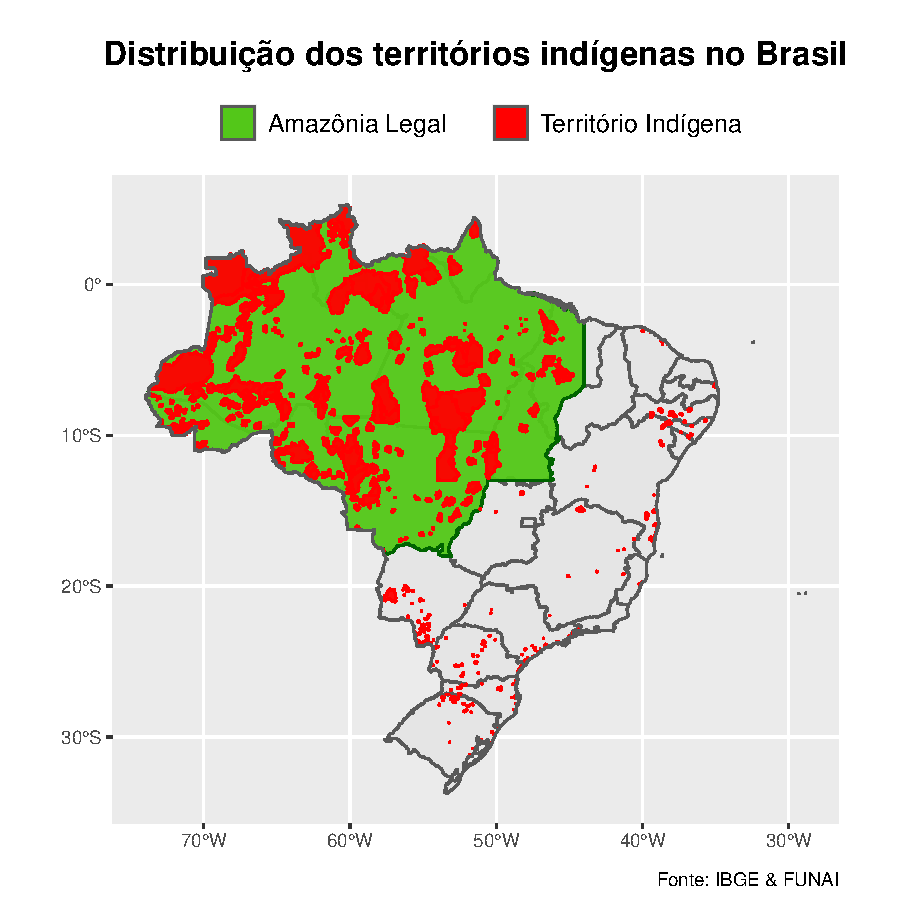
\includegraphics[width=0.8\linewidth]{indigenous_land_br}
\caption{Distribuição dos territórios indígenas no Brasil.}
\label{fig:territorio_indigena}
\end{figure}

As florestas tropicais, apesar de serem representarem um ecossistema rico em biodiversidade, apresentam poucos recursos para subsistência humana. Nestes ambientes, por exemplo, as plantas investem a maioria da sua energia para a manutenção de suas estruturas, gerando poucos frutos, que por sua vez serviriam de alimento para humanos e outros animais \cite{bailey_hunting_1989}.

A alta diversidade de plantas com troncos altos e copas largas, faz com que haja pouca penetração solar \cite{ratnam_when_2011}, que, aliado com a alta umidade e temperatura característica das florestas tropicais, atua como um fator de complicação para termorregulação \cite{perry_evolution_2009}. Ademais, a alta sazonalidade das florestas tropicais pode atrapalhar a caça, complicando ainda mais a subsistência humana \cite{hart_ecological_1986,bailey_hunting_1989}.

Além das complicações para obtenção de alimento e termorregulação, constata-se uma elevada patogenicidade nas florestas tropicais. Estima-se, por exemplo, que as florestas tropicais contenham cerca de 70\% de patógenos a mais que as florestas temperadas \cite{guernier_ecology_2004}. Como consequência disso e da falta de sistema de saúde adequado, constata-se uma alta mortalidade em povos indígenas, principalmente em crianças \cite{ohenjo_health_2006}.

Dado às diversas dificuldades para subsistência humana em florestas tropicais, somado à rápida expansão América do Sul adentro, questiona-se se é sequer possível que os habitantes destes ambientes tenham sobrevivido como caçadores-coletores, sem a dependência de recursos externos, como agricultura \cite{bailey_hunting_1989}. 

Tradicionalmente, compreende-se que as populações nativas da Amazônia foram constituídas por pequenas populações de caçadores-coletores. Cabe ressaltar, no entanto, que tem havido um crescente número de evidências que suportam a existência grandes sociedades \cite{heckenberger_amazonian_2009,de_souza_pre-columbian_2018}, centros de domesticação de plantas \cite{clement_origin_2010,clement_domestication_2015}, bem como um papel crucial dos rios como rotas primárias de migração \cite{arias_high-resolution_2018}. Ainda assim, o hábito caçador-coletor não só esteve presente, como foi essencial na história das populações nativas amazônicas, e ainda hoje encontram-se populações voluntariamente isoladas que vivem desta forma \cite{oliveira_cacadores_2007}. 

Não se sabe ainda ao certo qual a data aproximada do povoamento inicial da floresta amazônica, embora cada vez mais tenham surgido novos estudos que contribuem diretamente para esta área. Como mencionado acima, já na América do Sul, tem-se evidências concretas da presença humana há aproximadamente 14.000AP em Monte Verde, Chile \cite{dillehay_probing_2009}. Considerando que nativos-americanos adentraram a América do Sul pelo Istmo do Panamá, podemos considerar uma entrada bem anterior a isso, quer seja pela Amazônia ou pela região costeira do oceano pacífico \cite{potter_current_2018}. No referente à Amazônia, um estudo publicado ainda em 2020 mostra evidências da presença humana há aproximadamente 10 mil anos na planície beniana (Llanos de Moxos), localizada nas terras baixas da Bolívia, no sudoeste da Amazônia \cite{lombardo_early_2020}. Em acordo com outros estudos, esse artigo mostra um evento claro de nicho construído por populações nativo-americanas \cite{hunemeier_evolutionary_2012,watling_direct_2018}.

\subsection{Adaptação Local à Floresta Amazônica}

Os estudos de seleção na América do Sul são demasiadamente escassos na literatura. Se considerarmos a adaptação local à Floresta Amazônica, por exemplo, em nosso conhecimento, existem apenas dois estudos publicados até a presente data \cite{amorim_detection_2015,borda_genetic_2020}.

\citeonline{amorim_detection_2015} avaliaram as populações Suruí e Karitiana disponíveis no banco de dados do Human Genome Diversity Project (HGDP)  \cite{cann_human_2002,rosenberg_genetic_2002} a fim de comparar evolução convergente com outras populações de floresta tropical que vivem na África (\emph{e.g.} pigmeus). Com isso, identificaram sinais de seleção em genes relacionados ao sistema imunológico, metabolismo de lipídio, desenvolvimento corporal e resposta ao estresse. Em estudo recente, \citeonline{borda_genetic_2020}, utilizando uma amostra restrita de populações peruanas, realizaram testes de seleção em populações da Amazônia Peruana (Yunga) e das Terras Baixas Amazônicas, identificando como gene-candidato \textsl{PTPRC}, responsável pela produção da proteína CD45, que por sua vez atua diretamente no reconhecimento de patógenos, sobretudo virais \cite{borda_genetic_2020}. Assim, conforme esperado em ambientes com altos índices de patógenos \cite{guernier_ecology_2004}, ambos os estudos publicados até o momento convergiram em seus achados, identificando com os maiores sinais seletivos genes-candidatos responsáveis pela resposta imunológica.

A maioria dos estudos de adaptação local na América tem focado nos Andes (vide Capítulo \ref{chap:andes}). Demais estudos têm focado na Mesoamérica \cite{hunemeier_evolutionary_2012}, na Groenlândia \cite{fumagalli_greenlandic_2015}, ou mesmo na América como um todo, no contexto do período de parada na Beríngia e povoamento das Américas \cite{acuna-alonzo_functional_2010,amorim_genetic_2017}. Contrariamente à escassez de pesquisa sobre adaptação local à Floresta Tropical Amazônica, existem numerosas pesquisas avaliando adaptação local a outras florestas tropicais, sobretudo na África. Estes estudos tornam-se valiosos para esta tese, uma vez que servem como base de comparação.

Este trabalho tem como objetivo investigar a influência da seleção natural na populações nativas americanas da floresta amazônica, por meio (1) da identificação de SNPs e genes candidatos à seleção positiva; (2) da análise de vias e de redes de genes candidatos à seleção positiva; e (3) da caracterização das possíveis pressões seletivas exercidas sobre os genes e vias identificados.

\clearpage
\section{MATERIAL E MÉTODOS} 

\subsection{Populações}

Para o estudo de adaptação local à Floresta Tropical Amazônica, utilizamos dois conjuntos de dados principais, provenientes de diferentes arranjos de genotipagem (Axiom Human Origins e Illumina), aqui nomeados como dataset S1 e dataset S2, respectivamente. O primeiro e principal conjunto de dados contém amostras de 118 nativos Amazônicos, resultados da junção de 37 indivíduos genotipados para este projeto (27 Xavantes, 7 Xikrin, 2 Munduruku e 1 Asurini), 48 indivíduos do estudo de \cite{skoglund_genetic_2015},  12 indivíduos de \cite{castro_e_silva_genomic_2020}, e 21 indivíduos do dataset 11 provenientes do projeto HGDP (\url{http://www.cephb.fr/hgdp/}). Aproveitamos também este último para aquisição de indivíduos nativos da Mesoamérica (n = 35) e do leste da asiático (n = 231) para fins de análises de seleção, bem como populações de outros continentes para análise de estruturação populacional. Todas as populações nativas americanas, bem como os grupos utilizados para as análises de seleção podem ser verificadas nas tabelas \ref{tab:ds1_natives} e \ref{tab:ds1_selgroups}, respectivamente.

O segundo conjunto de dados contém 104 indivíduos nativos amazônicos e 81 nativos andinos, provenientes do estudo de \citeonline{gnecchi-ruscone_dissecting_2019}, somados aos dados de sequenciamento completo do Simons Genome Diversity Project ─ SGDP \cite{mallick_simons_2016} e de \citeonline{bergstrom_insights_2020}, incluindo 63 indivíduos nativos da Mesoamérica, e aproximadamente mil indivíduos dos demais continentes. Os indivíduos nativos amazônicos e os grupos utilizados nas análises de seleção são apresentados nas Tabelas \ref{tab:ds2_natives} e \ref{tab:ds2_selgroups}, respectivamente.

\subsection{Filtros de Qualidade e Faseamento do Genoma}

Para ambos os conjunto de dados, aplicamos os mesmos filtros de qualidade utilizando o software PLINK v1.9 \cite{chang_second-generation_2015}, que consistiram na remoção de indivíduos com mais de 10\% de dados faltantes (flag --mind 0.1) e remoção de SNPs com MAF menor que 5\% ou com mais de 1\% de dados faltantes nos indivíduos (flags --maf 0.05 e --geno 0.01, respectivamente), quando considerado o conjunto de dados como um todo. Adicionalmente, para os dados de sequenciamento utilizados no dataset S2, removemos todas as variantes cujos alelos eram A e T ou C e G, bem como aquelas com \textit{Phred score} menor que 40. Como resultado, os conjuntos de dados finais apresentaram 523.319 e 612.293 SNPs, respectivamente. 
A fim de realizar as análises de varredura genômica, utilizamos o software SHAPEIT \cite{delaneau_linear_2012} com os argumentos-padrão para fasear os conjuntos de dados, utilizando como mapa de recombinação os dados do Projeto 1000 Genomas \cite{1000_genomes_project_consortium_global_2015}. Adicionalmente, uma vez que abordagens específicas de seleção requerem a diferenciação dos alelos ancestrais (\emph{e.g.} iHS), utilizamos também os dados do Projeto 1000 Genomas (\url{http://ftp.1000genomes.ebi.ac.uk/vol1/ftp/phase1/analysis_results/supporting/ancestral_alignments/}) para ajustar os alelos ancestrais, descartando as variantes sem anotação disponível, o que resultou em 517.984 e 601.648 SNPs para as análises derivadas da EHH (vide tópico \ref{subsec:amazonia_methods_ehh}).

\vspace{\onelineskip}

% tabela 2.1
\begin{table}[htb!]
\centering

\renewcommand\theadalign{cl}
\renewcommand\theadfont{\mdseries}
\renewcommand\theadgape{\Gape[4pt]}
\renewcommand\cellgape{\Gape[4pt]}

\newcommand{\specialcell}[2][c]{%
  \begin{tabular}[#1]{@{}c@{}}#2\end{tabular}}

%\resizebox{\linewidth}{!}{
\begin{tabular}[htb!]{lllrrlr}
\toprule
\thead{População} & \thead{Grupo\\Linguístico} & \thead{Região} & \thead{Latitude} & \thead{Longitude} & \thead{Referência} & \thead{N}\\
\midrule
\cellcolor{gray!6}{Apalai} & \cellcolor{gray!6}{Karib} & \cellcolor{gray!6}{Brasil} & \cellcolor{gray!6}{-1.33} & \cellcolor{gray!6}{-54.67} & \cellcolor{gray!6}{Skoglund} & \cellcolor{gray!6}{4}\\
Arara & Karib & Brasil & -3.91 & -53.59 & Skoglund & 4\\
\cellcolor{gray!6}{Asurini} & \cellcolor{gray!6}{Tupi} & \cellcolor{gray!6}{Brasil} & \cellcolor{gray!6}{-3.89} & \cellcolor{gray!6}{-51.05} & \cellcolor{gray!6}{Este} & \cellcolor{gray!6}{1}\\
Gavião & Jê & Brasil & -10.17 & -61.13 & Castro e Silva & 2\\
\cellcolor{gray!6}{Guarani\_GN} & \cellcolor{gray!6}{Tupi} & \cellcolor{gray!6}{Brasil} & \cellcolor{gray!6}{-23.33} & \cellcolor{gray!6}{-54.50} & \cellcolor{gray!6}{Skoglund} & \cellcolor{gray!6}{7}\\
Guarani\_KW & Tupi & Brasil & -23.33 & -55.20 & Skoglund & 10\\
\cellcolor{gray!6}{Guarani\_Mbya} & \cellcolor{gray!6}{Tupi} & \cellcolor{gray!6}{Brasil} & \cellcolor{gray!6}{-23.10} & \cellcolor{gray!6}{-55.00} & \cellcolor{gray!6}{Castro e Silva} & \cellcolor{gray!6}{4}\\
Karitiana & Tupi & Brasil & -8.75 & -63.84 & Skoglund/HGDP & 17\\
\cellcolor{gray!6}{Munduruku} & \cellcolor{gray!6}{Tupi} & \cellcolor{gray!6}{Brasil} & \cellcolor{gray!6}{-6.38} & \cellcolor{gray!6}{-59.15} & \cellcolor{gray!6}{Este} & \cellcolor{gray!6}{2}\\
Parakanã & Tupi & Brasil & -5.37 & -51.28 & Castro e Silva & 3\\
\cellcolor{gray!6}{Surui} & \cellcolor{gray!6}{Tupi} & \cellcolor{gray!6}{Brasil} & \cellcolor{gray!6}{-11.00} & \cellcolor{gray!6}{-62.00} & \cellcolor{gray!6}{Skoglund/HGDP} & \cellcolor{gray!6}{12}\\
Tupiniquim & Tupi & Brasil & -19.88 & -40.18 & Castro e Silva & 1\\
\cellcolor{gray!6}{Urubu\_Kaapor} & \cellcolor{gray!6}{Tupi} & \cellcolor{gray!6}{Brasil} & \cellcolor{gray!6}{-2.50} & \cellcolor{gray!6}{-46.50} & \cellcolor{gray!6}{Skoglund} & \cellcolor{gray!6}{3}\\
Wajãpi & Tupi & Brasil & 1.05 & -52.83 & Castro e Silva & 2\\
\cellcolor{gray!6}{Xavante} & \cellcolor{gray!6}{Jê} & \cellcolor{gray!6}{Brasil} & \cellcolor{gray!6}{-14.00} & \cellcolor{gray!6}{-52.50} & \cellcolor{gray!6}{Skoglund/Este} & \cellcolor{gray!6}{38}\\
Xikrin & Jê & Brasil & -5.92 & -51.00 & Este & 7\\
\cellcolor{gray!6}{Zoro} & \cellcolor{gray!6}{Tupi} & \cellcolor{gray!6}{Brasil} & \cellcolor{gray!6}{-10.33} & \cellcolor{gray!6}{-60.33} & \cellcolor{gray!6}{Skoglund} & \cellcolor{gray!6}{1}\\
Maya & Mayan & México & 19.00 & -91.00 & HGDP & 21\\
\cellcolor{gray!6}{Pima} & \cellcolor{gray!6}{Uto-Aztecan} & \cellcolor{gray!6}{México} & \cellcolor{gray!6}{29.00} & \cellcolor{gray!6}{-108.00} & \cellcolor{gray!6}{HGDP} & \cellcolor{gray!6}{14}\\
\bottomrule
\end{tabular}%}
\caption{Nativos Americanos ─ Dataset S1.}
\label{tab:ds1_natives}

\end{table}


\vspace{\onelineskip}

% tabela 2.2
\begin{table}[htb!]
\centering
\begin{tabular}[htb!]{llr}
\toprule
Grupo & Macrorregião & N\\
\midrule
Amazônia & América do Sul & 118\\
Lesta da Ásia & Ásia & 231\\
Mesoamérica & América Central & 35\\
\bottomrule
\end{tabular}

\caption{Grupos utilizados nas análises de seleção ─ Dataset S1.}
\label{tab:ds1_selgroups}

\end{table}


% tabela 2.3
\begin{table}[htbp!]
\centering

\newcolumntype{M}{>{\centering\arraybackslash}m{3.1cm}}
\newcolumntype{R}{>{\raggedleft\arraybackslash}m{0.5cm}}

\begin{tabular}[htb!]{m{3.5cm}m{2cm}m{3cm}m{3cm}R}

\toprule
População & País & Ecorregião & Referência & N\\
\midrule
\addlinespace[0.3em]
\multicolumn{5}{l}{\textbf{América do Sul}}\\
\midrule
\addlinespace[0.3em]
Ashaninka & Peru & Amazonia & GnecchiRuscone & 9\\
Cashibo & Peru & Amazonia & GnecchiRuscone & 9\\
Huambisa & Peru & Amazonia & GnecchiRuscone & 6\\
Karitiana & Brazil & Amazonia & HGDP3 & 12\\
Shipibo & Peru & Amazonia & GnecchiRuscone & 14\\
Surui & Brazil & Amazonia & HGDP3 & 8\\
Yanesha & Peru & Amazonia & GnecchiRuscone & 46\\
\addlinespace[0.3em]

\midrule
\multicolumn{5}{l}{\textbf{Mesoamérica}}\\
\midrule
\addlinespace[0.3em]
Maya & Mexico & Mesoamerica & HGDP3 & 20\\
Mixe & Mexico & Mesoamerica & SGDP & 3\\
Mixtec & Mexico & Mesoamerica & SGDP & 2\\
Pima & Mexico & Mesoamerica & HGDP3 & 13\\
Tzotzil & Mexico & Mesoamerica & GnecchiRuscone & 23\\
Zapotec & Mexico & Mesoamerica & SGDP & 2\\
\bottomrule

\end{tabular}

\caption{Nativos Americanos ─ Dataset S2.}
\label{tab:ds2_natives}

\vspace{\onelineskip}

\end{table}



\FloatBarrier

% tabela 2.4
\begin{table}[htbp!]
\centering

\setlength\extrarowheight{1pt}

\centering
\begin{tabular}[htb!]{p{3cm}p{3.5cm}r}
\toprule
Grupo & Macrorregião & N\\
\midrule
Amazônia & América do Sul & 104\\
Leste da Ásia & Ásia & 225\\
Mesoamérica & América Central & 63\\ [0.1ex] 
\bottomrule
\end{tabular}

\caption{Grupos utilizados nas análises de seleção ─ Dataset S2.}
\label{tab:ds2_selgroups}

\end{table}


\FloatBarrier

\subsection{Anotação do Genoma}

Realizamos a anotação do genoma com o software ANNOVAR \cite{wang_annovar_2010}, bem como uso de scripts personalizados. Os genes foram atribuídos a cada SNP utilizando como referência o banco RefGene, fornecido pelo próprio software ANNOVAR.  Para anotação da identificação dos SNPs (dbSNP), utilizamos as identificações providas pelo site comercial do arranjo Axiom Human Origins (\url{https://www.thermofisher.com/br/en/home/life-science/microarray-analysis/microarray-data-analysis/genechip-array-annotation-files.html}) para o  dataset S1, e as aquelas providas pelo banco de dados do 1000G para o dataset S2. Adicionalmente, removemos a anotação dos genes alocados a mais de 10 kb do SNP-alvo.

\subsection{Estrutura Populacional}

Para análise da estrutura populacional, aplicamos análise de PCA em ambos os datasets, utilizando o software Plink v1.9 \cite{chang_second-generation_2015}, após filtro de desequilíbrio de ligação com 50 SNPs para cada janela, deslizando de 5 em 5 SNPs, mantendo apenas os SNPs com correlação inferior a 20\%, utilizando o mesmo programa.

A análise de miscigenação foi realizada com o software ADMIXTURE \cite{alexander_fast_2009}, adotando uma abordagem não-supervisionada com dez corridas independentes, utilizando amazônicos, europeus e africanos subsaarianos. Para identificar exclusivamente se há componentes europeus ou africanos nos nativos amazônicos (e não subestruturação dentro da Amazônia ou nos continentes analisados), reportamos a análise com os três componentes. Utilizamos o software pong \cite{behr_pong_2016} para pós-processamento das corridas e produção do gráfico. 

\subsection{Varreduras Seletivas}
\label{subsec:amazonia_methods_ehh}

Foram aplicados três testes para detecção de sinais de seleção positiva, que diferem em sua abordagem estatística principal. O primeiro, PBS, possui como princípio estatístico a subestruturação populacional por meio do cálculo de Fst. Os dois seguintes, iHS e XP-EHH, baseiam-se no decaimento da extensão de homozigose do haplótipo (EHH). Enquanto iHS, como método intra-populacional, tem-se mostrado mais apropriado na detecção de sweeps incompletos, XP-EHH compara a população-alvo com uma população-irmã e detecta de forma mais robusta sweeps completos (ou muitos próximos da fixação) \cite{suzuki_statistical_2010}. 

Em ambos os datasets, estruturamos a análise de PBS utilizando os amazônicos como população focal, mesoamericanos como população-irmã, e asiáticos do leste como grupo externo. Realizamos a inferência de PBS como originalmente descrito por \cite{yi_sequencing_2010}, utilizando o índice Fst de \cite{reynolds_estimation_1983} nos dados previamente faseados. Adicionalmente, rodamos uma média móvel por janela utilizando 20 SNPs em cada janela, ao passo que 5 SNPs. Para cada janela, apenas o SNP com maior valor de PBS, bem como suas informações associadas (\emph{e.g.} cromossomo, posição, dbSNP e gene) foram mantidos. Para identificar os SNPs e genes candidatos, utilizamos duas abordagens distintas: 1) por SNP e 2) por gene. Na abordagem por SNP, selecionamos os SNPs cujo valor de PBS é igual ou superior ao quantil de 0,999, ou seja, os top 0,1\% da distribuição (\emph{p}-valor unicaudal empírico < 0,001). Na análise por gene, calculamos a média de PBS por gene e, nesta distribuição, de maneira similar à abordagem por SNP, selecionamos como top 0,1\% dos genes na distribuição como genes candidatos. Em ambas as abordagens, calculamos o \emph{p}-valor empírico unilateral dos dados considerando a proporção de valores maiores ou iguais ao valor-alvo, corrigindo para amostra finita. Uma maneira de fazer isso, é utilizando a fórmula $p = (1 + \sum s \geq s_i)/(N + 1)$, onde $s$ é o vetor de valores, $s_i$ o valor-alvo, e $N$ o tamanho do vetor. Outra maneira, utilizando o mesmo princípio, consiste em primeiro ranquear os valores-alvos, possibilitando o uso da vetorização com o pacote data.table em R, através da fórmula $p = 1 - r/(N+1)$, onde $r$ consiste no valor ranqueado proveniente da função frank do pacote data.table do R. Optamos pela segunda opção, visto que é mais de 4.000 vezes mais rápida que a primeira. Adicionalmente, computamos o logaritmo negativo dos \emph{p}-valores, na base 10, onde um \emph{p}-valor de 0,01 equivale a 2. 

Nas análises derivadas de EHH, utilizamos os dados previamente faseados e polarizados (corrigidos para o alelo ancestral) como entrada para as funções do pacote rehh do R \cite{gautier_rehh_2012,gautier_rehh_2017}, utilizando os valores-padrão das funções \emph{ihh2ihs} e \emph{ies2xpehh}  para realizar as inferências dos valores normalizados de iHS e XP-EHH, respectivamente. Em ambos os datasets, a análise de XP-EHH foi estruturada utilizando os amazônicos como população-alvo e os mesoamericanos como população-irmã, ao passo que iHS, como método intra-populacional, utilizou-se apenas os amazônicos. Adicionalmente, para o método iHS, transformamos os valores inferidos em valores absolutos, uma vez que tanto valores negativos quanto positivos são indicativos de seleção. De maneira similar ao método PBS, calculamos \emph{p}-valores empíricos e aplicamos a abordagem de detecção por SNP e por gene para identificar SNPs e genes candidatos, focando no extremo 0,1\% da distribuição (\emph{i.e.} \emph{p}-valor de 0,001). 

Aqui, optamos por realizar tanto a abordagem por SNP quanto por gene como meio de identificar os SNPs e genes candidatos porque ambas possuem suas vantagens e desvantagens. Ao passo que a abordagem por SNP ─ segundo \cite{weng_snp-based_2011}, a mais utilizada nas análises de enriquecimento gênico ─ pode representar com maior fidelidade a relevância dos SNPs identificados dado seus valores extremos, os SNPs identificados representam apenas uma pequena fração das variantes genéticas que contribuem para fenótipos complexos \cite{shriner_problems_2007}, além de que, genes maiores podem apresentar SNPs com altos valores por acaso. Na abordagem por gene, por sua vez, ao passo que captura todos os valores de SNPs por gene, genes com SNPs que apresentam alta variância tendem a ser ignorados. De forma resumida, a abordagem por SNP pode resultar em falsos positivos, ao passo que a abordagem por gene tende a apresentar falsos negativos. Os ruídos dos SNPs falsos positivos, contudo, são drasticamente diminuídos pela abordagem da média em janelas móveis.

Os resultados provenientes das varreduras genômicas foram utilizados também para construir uma lista de genes para as análises de super-representação gênica (ORA) e enriquecimento gênico (GSEA). Nestes casos, como uma quantidade maior de genes candidatos foi encontrada, selecionamos nestas análises apenas aqueles cujos \emph{p}-valores correspondentes (corrigidos por FDR) eram significativos a um nível de 5\%, definimos, também, diferentes valores de corte da distribuição além dos extremos 0,1\%, como 0,5\% e 1\%, resultando em diferentes conjuntos de genes candidatos (vide item \ref{subsec:amazonia_methods_annotfuncional}). Adicionalmente, para cada conjunto de SNPs e genes candidatos, realizamos o teste não-paramétrico de Wilcoxon \cite{wilcoxon_individual_1945} a fim de verificar se estes candidatos estão significativamente distantes da mediana da distribuição, visto que, em todos os casos (ambos datasets para três métodos), os dados possuem distribuição não-normal (teste de Shapiro-Wilk $< 2,2^{-16}$).

\subsection{Anotação Funcional}
\label{subsec:amazonia_methods_annotfuncional}

A fim de compreender as funções biológicas dos SNPs e genes candidatos, utilizamos três banco de dados - Ensembl \cite{yates_ensembl_2015}, GWAS Catalog \cite{buniello_nhgri-ebi_2019,macarthur_new_2017} e GeneCards \cite{stelzer_genecards_2016} - para mapear os fenótipos associados aos genes candidatos. Para isso, utilizamos a REST API tanto do Ensembl quanto do GWAS Catalog para realizar as nossas buscas.

Além da anotação de fenótipos derivados dos genes candidatos, realizamos uma busca mais específica focando nos alelos-alvo dos SNPs candidatos utilizando o banco de dados GTEx \cite{gtex_consortium_genotype-tissue_2013}. Nesta análise, selecionamos apenas os alelos dos SNPs candidatos com maior frequência na população amazônica quando comparado aos mesoamericanos, previamente identificados pelos métodos PBS e XP-EHH (\emph{p}-valor < 0,01), e então buscamos seus valores eQTL para os respectivos genes utilizando a REST API do banco GTEx \cite{gtex_consortium_genotype-tissue_2013}, para cada um dos 48 tecidos disponíveis na versão “gtex\_v7” (referente à versão do genoma Grch37), mantendo apenas aqueles cujo \emph{p}-valor de eQTL é menor que 0,01. Uma vez que não é possível distinguir programaticamente o papel biológico do aumento ou diminuição da expressão dos genes no tecidos, reportamos tanto a contagem de alelos-alvo para o aumento (\textit{up}) ou diminuição (\textit{down}) da expressão nos tecidos, como também somamos a contagem do aumento e diminuição por tecido para verificar em quais tecidos os alelos candidatos estão mais expressos, independentemente da maneira de expressão (promovendo ou reprimindo). 

\subsection{Enriquecimento Gênico}

Posteriormente às análises de varreduras genômicas, realizamos análises de super-representação gênica (ORA) e enriquecimento gênico (GSEA) utilizando quatro plataformas: Enrichr \cite{chen_enrichr_2013,kuleshov_enrichr_2016}, FUMAGWAS \cite{watanabe_functional_2017}, WebGestalt \cite{zhang_webgestalt_2005,wang_webgestaltr_2020}, e GOATOOLS \cite{klopfenstein_goatools_2018}, focando em três bancos de dados: GWAS Catalog \cite{macarthur_new_2017}, KEGG Pathway \cite{kanehisa_kegg_2000} e Gene Ontology \cite{ashburner_gene_2000,thegeneontologyconsortium_gene_2019}. Optamos primeiramente por Enrichr para analisar os bancos de dados GWAS Catalog e KEGG, uma vez que o mesmo contém uma API em Python, GSEApy \cite{fang_gseapy_2020}, possibilitando a análise em conjunto dos diferentes grupos de genes candidatos mais facilmente. Contudo, uma vez que o mesmo não possibilita o uso de uma lista de população gênica personalizada (utilizando os genes do SNP-Array), utilizamos também os softwares FUMAGWAS e WebGestalt para análise nos bancos GWAS Catalog e KEGG Pathway, respectivamente, especificando como população gênica os genes disponíveis em nossos dados (Affymetrix e Illumina para os datasets S1 e S2, respectivamente). Para análise de enriquecimento de termos GO, utilizamos a ferramenta GOATOOLS. Dado que esta biblioteca possibilita múltiplas manipulações e agrupamentos dos termos GO, analisamos tanto o conjunto completo dos termos GO relacionados aos processos biológicos, bem como sua versão não-redundante (GO slim), e termos específicos do sistema imunológico. Neste programa, selecionamos como método de correção dos \emph{p}-valores a implementação de FDR baseada em reamostragem (\emph{resampling-based FDR}), disponibilizado pelo próprio programa, enquanto para as demais plataformas utilizamos a correção padrão de FDR. Para todos os softwares, selecionamos como genes candidatos aqueles identificados no extremo 0,1\%, 0,5\% e 1\% superior à distribuição de ambas as abordagens por SNP e por gene.

\subsection{Convergência Evolutiva}

Para análise de convergência evolutiva, selecionamos todos os artigos de seleção em populações nativas de Floresta Tropicais disponíveis, totalizando 13 estudos. Para cada estudo, anotamos as populações-alvo e os métodos aplicados, e selecionamos os genes candidatos reportados (outliers), geralmente disponíveis na seção de material suplementar. Verificamos e reportamos então a interseção dos genes candidatos levantados nestes trabalhos e dos genes candidatos levantados em nossa pesquisa, tanto de forma individual (por artigo) como de forma unificada (todos artigos em conjunto). Para cada gene em intersecção anotamos os fenótipos associados como descrito no item \ref{subsec:amazonia_methods_annotfuncional}, e agrupamos estes fenótipos para poder ter uma melhor compreensão daqueles mais frequentes, bem como as informações associadas aos mesmos (quantidade de estudos, genes e positividade nos métodos aplicados).

\subsection{Disponibilização dos Dados e Códigos}

Considerando os conjuntos de dados filtrados e faseados, todos os scripts utilizados nesta pesquisa se encontra disponível no link \url{https://github.com/cmcouto-silva/tese}, organizados para reprodutibilidade via Snakemake \cite{koster_snakemake--scalable_2012}, um sistema de gerenciamento de fluxo de trabalho (\textit{workflow}) baseado em Python comumente utilizado na área da bioinformática. Todas as dependências para execução do \textit{workflow} (\emph{e.g.} R, Python e softwares de bioinformática) estão disponíveis tanto via Docker container (\url{https://hub.docker.com/repository/docker/cmcoutosilva/tese}) quanto arquivo de configuração para ambiente virtual conda (ANACONDA SOFTWARE DISTRIBUTION, 2021). As figuras e tabelas resultantes desta pesquisa estão disponíveis no repositório de dados do Mendeley (\url{http://dx.doi.org/10.17632/gztff7wmjt.1}).

%% ------------------------------------------------------------------------- %%
%% ------------------------------ RESULTADOS ------------------------------- %%
%% ------------------------------------------------------------------------- %%

\section{RESULTADOS}

\subsection{Estrutura Populacional}

A distribuição atual das populações nativas americanas presentes no dataset S1 pode ser verificada na figura \ref{fig:ds1_nam_map}. Cabe ressaltar que mesmo as populações que já não se encontram atualmente na região Amazônica passaram e muito provavelmente permaneceram nela por um longo tempo formativo. Pode-se observar que estas populações se agrupam de maneira distante das populações européias e africanas, estando mais próximas às populações Mesoamericanas e do leste Asiático, padrão que se repete no dataset S2 (\autoref{fig:ds1_pca_admx}A-B). 

\begin{figure}[!htbp]
\noindent
\centering
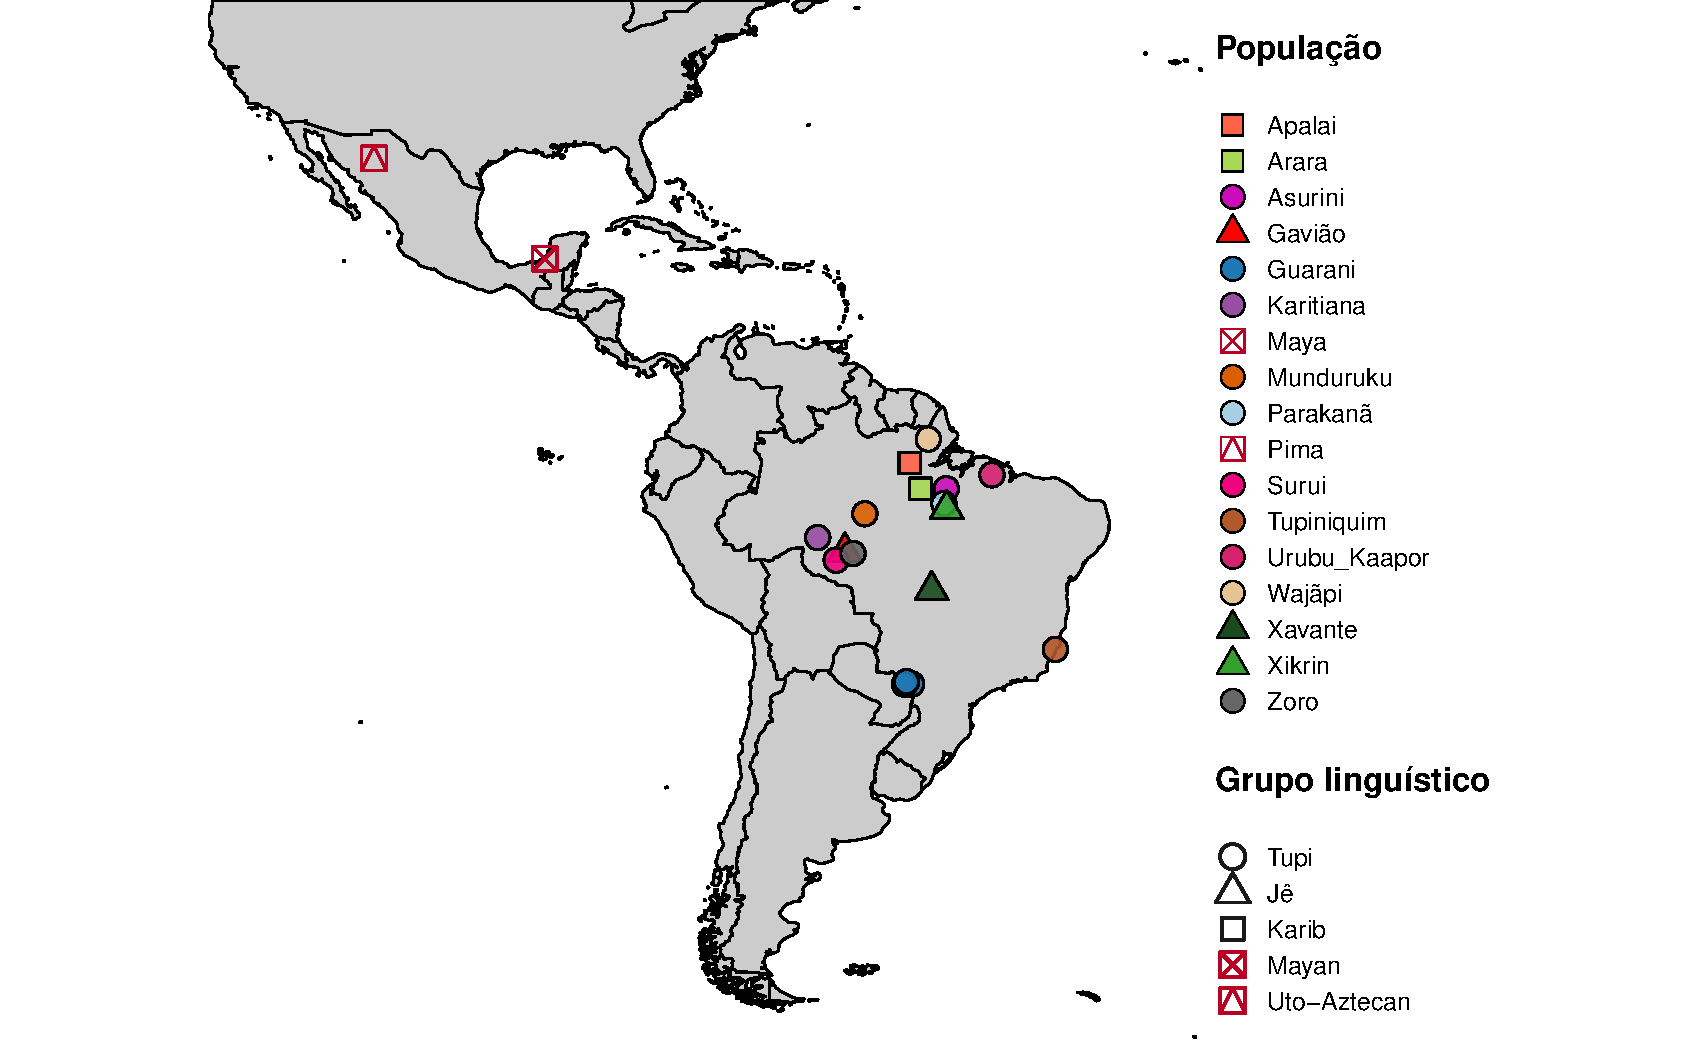
\includegraphics[width=1\linewidth]{ds1_nam_map}
\caption{Distribuição das populações nativas Americanas analisadas.}
\label{fig:ds1_nam_map}
\end{figure}

Para avaliar possível miscigenação dos nativos Amazônicos em nosso estudo, utilizamos ADMIXTURE com populações da África Subsaariana e Europa, dividindo em três componentes (\autoref{fig:ds1_pca_admx}C). Com exceção de possíveis ruídos nos primeiros nativos amazônicos, não se observam componentes presentes em Africanos e Europeus. A miscigenação e dispersão dos nativos Amazônicos do dataset S2 pode ser verificada diretamente no artigo de \citeonline{gnecchi-ruscone_dissecting_2019}.

\begin{figure}[!htb]  % figura 2.2
\noindent
\centering
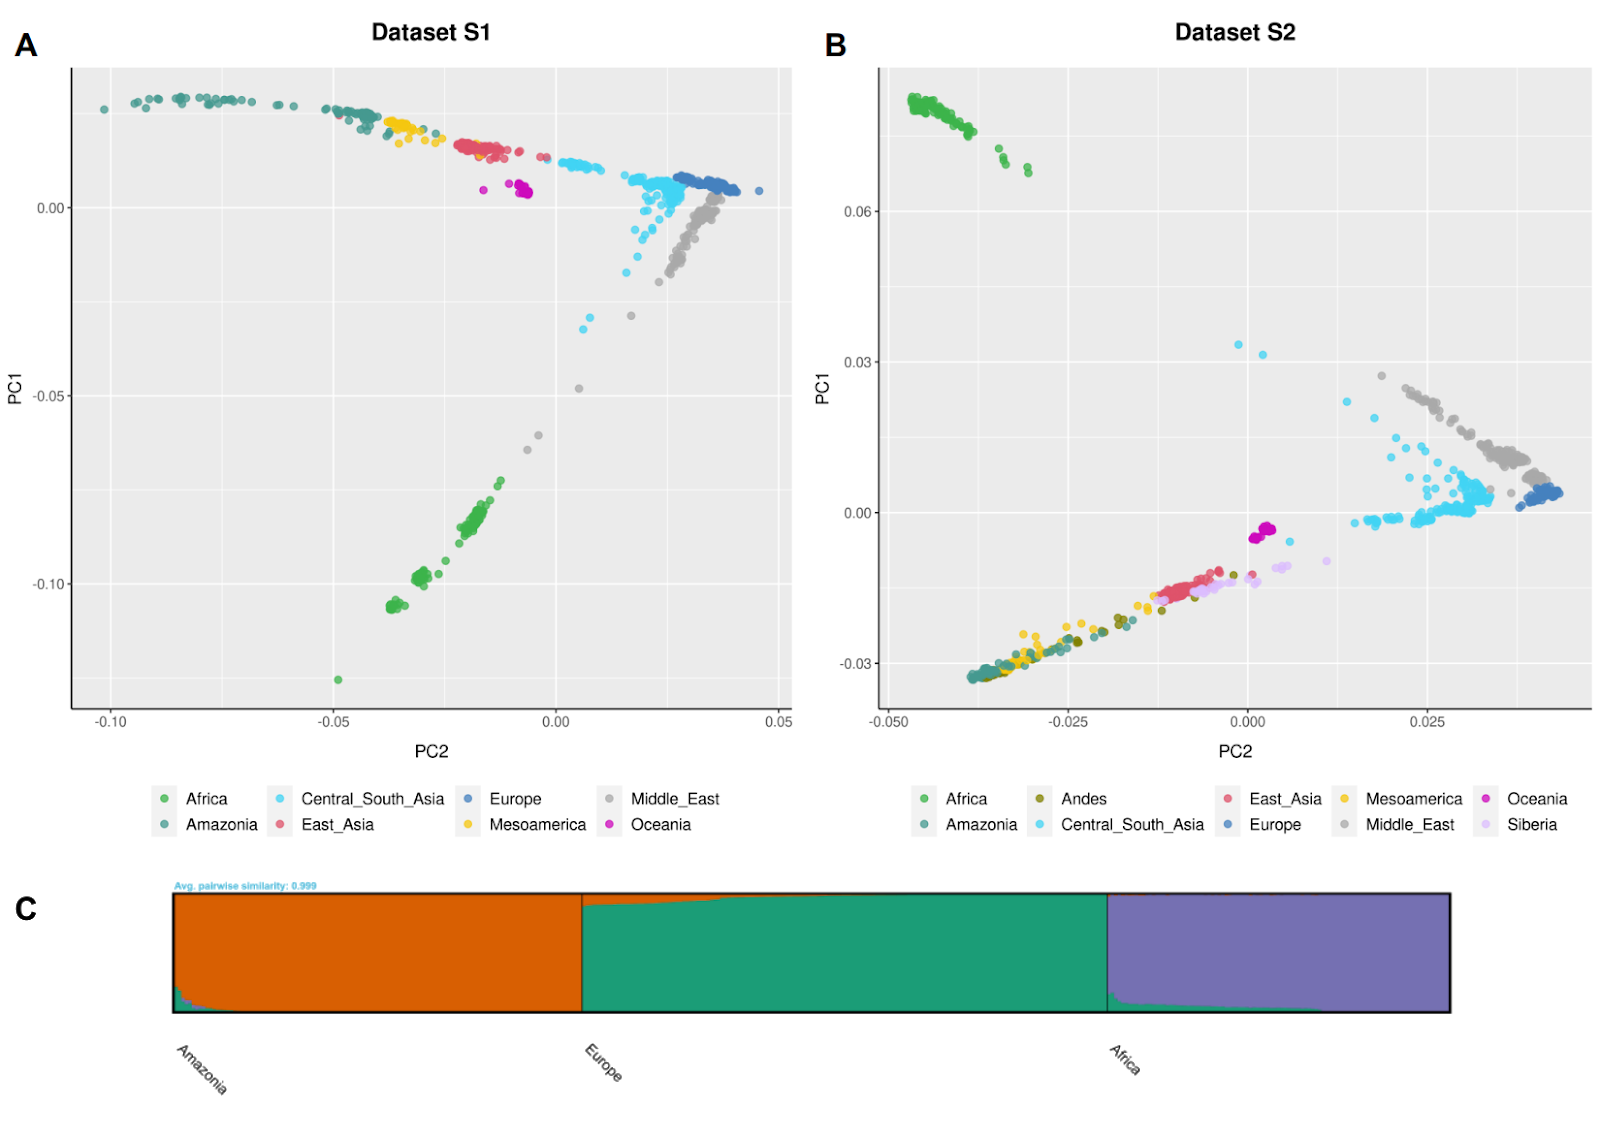
\includegraphics[width=1\linewidth]{ds1_pca_admx}
\caption[Análise de PCA e ADMIXTURE.]{Análise de PCA e ADMIXTURE. (A) PCA para o dataset S1 e (B) dataset S2, englobando todas as populações disponíveis nos respectivos datasets. (C) Análise não-supervisionada de miscigenação no dataset S1, utilizando três componentes (K = 3).}
\label{fig:ds1_pca_admx}
\end{figure}

\subsection{Varreduras Seletivas}

Nós computamos três estatísticas inferenciais de seleção que contém propriedades complementares para detecção de eventos adaptativos: PBS, iHS e XP-EHH. Partindo pela análise de PBS, estruturamos a análise com os nativos amazônicos como população focal, nativos da Mesoamerica como população próxima, e populações do Leste Asiático como grupo externo, calculando uma média móvel por janelas deslizantes de 20 SNPs movendo a cada 5 SNPs (vide item \ref{subsec:amazonia_methods_ehh}). Através dessa abordagem, identificamos 29 SNPs com \emph{p}-valor empírico < 0,001, dentro ou próximos de 31 genes no dataset S1 (\autoref{tab:ds1_pbsw_persnp}). Os genes correspondentes aos SNPs com valores mais altos dentro dessa distribuição, por cromossomo, estão representados na \autoref{fig:ds1_pbsw_both}A. Adicionalmente, calculamos a média dos valores de PBS para cada gene, e recalculamos \emph{p}-valores empíricos para a nova distribuição, resultando em 12 genes com \emph{p}-valor menor que 0,01 (\autoref{fig:ds1_pbsw_both}B). Cabe ressaltar que, dado que selecionamos valores extremos na distribuição, todos os valores extremos identificados tanto nas análises de PBS como nas seguintes (\emph{i.e.} iHS e XP-EHH) são significativamente diferentes da mediana observada para a respectiva distribuição (maior \emph{p}-valor para o teste Wilcoxon foi de $< 2,2^{-16}$).

Repetimos as análises de PBS para o dataset S2, identificando 26 genes na análise por SNP, e 13 genes na análise por gene (Tabelas \ref{tab:ds2_pbsw_persnp}-\ref{tab:pbsw_pergene}, \autoref{fig:pbs_intersection}). Destes, encontramos uma intersecção do gene \textsl{ACACA} abordagem por SNP (considerando \textsl{ACACA} no dataset S2), e \textsl{PDK4} na abordagem por gene. Se permitimos a identificação de \textit{outliers} acima do quantil 0,995 ao invés de 0,999, identificamos então 16 genes em intersecção na abordagem por SNP (incluindo \textsl{ACACA}, \textsl{DOCK2}, \textsl{MEGF11}, \textsl{PLXNA4} e  \textsl{NEB}), e 6 genes na abordagem por gene, incluindo \textsl{ACACA} e \textsl{PDK4} (\autoref{fig:pbs_intersection}).

\begin{table}[!htbp]
\centering
\resizebox{\linewidth}{!}{
\begin{tabular}[t]{crlllrr}
\toprule
CHR & POS & SNP & GENE & FUNÇÃO & PBS & -log$_{10}(p)$\\
\midrule
1 & 162060864 & rs10918593 & NOS1AP & intergenic & 0.2458 & 3.7893\\
2 & 25447908 & rs13390436 & DTNB & intronic & 0.2481 & 3.8437\\
2 & 152438741 & rs76206843 & FMNL2 & intronic & 0.2346 & 3.5726\\
2 & 162146324 & rs11897425 & LOC101929532 & ncRNA\_intronic & 0.1975 & 3.2136\\
2 & 162342778 & rs2033300 & GCA & intronic & 0.2273 & 3.5284\\
3 & 10260685 & rs451952 & TATDN2 & intronic & 0.1956 & 3.1625\\
4 & 101198533 & rs2659540 & PPP3CA & intronic & 0.3074 & 4.7188\\
4 & 109860572 & rs12498239 & LRIT3 & intronic & 0.1911 & 3.0955\\
5 & 7897170 & Affx-27022154 & MTRR & exonic & 0.2617 & 3.9058\\
5 & 10263613 & rs2244964 & CCT5 & intronic & 0.1910 & 3.0904\\
5 & 78395121 & rs1864172 & SCAMP1 & intronic & 0.1904 & 3.0853\\
5 & 169742629 & rs12514018 & DOCK2 & intronic & 0.2861 & 4.2416\\
6 & 46279855 & rs1442227 & LOC101926915 & ncRNA\_intronic & 0.1946 & 3.1506\\
6 & 154229719 & rs9397697 & IPCEF1,OPRM1 & intronic,intronic & 0.2475 & 3.8157\\
6 & 154400423 & rs6917661 & CNKSR3 & UTR3 & 0.2347 & 3.5884\\
6 & 170578141 & rs7745933 & PDCD2 & intronic & 0.1854 & 3.0375\\
7 & 69664093 & rs2533434 & AUTS2 & intronic & 0.2376 & 3.7188\\
7 & 95872168 & rs12535988 & DYNC1I1 & intronic & 0.2107 & 3.3385\\
7 & 135973421 & rs7801598 & LUZP6,MTPN & intronic,intronic & 0.1976 & 3.2204\\
8 & 118416705 & rs4077747 & SAMD12 & intronic & 0.2920 & 4.3208\\
10 & 77465512 & rs607483 & KCNMA1 & intronic & 0.2366 & 3.6581\\
11 & 125204544 & rs585974 & PKNOX2 & intronic & 0.1961 & 3.1873\\
13 & 31904154 & rs3848084 & EEF1DP3 & ncRNA\_intronic & 0.2142 & 3.3666\\
13 & 110395003 & rs7326145 & COL4A2 & intronic & 0.1932 & 3.1333\\
15 & 66135032 & rs55648467 & MEGF11 & intronic & 0.1840 & 3.0112\\
15 & 78266167 & rs2037347 & DNAJA4 & intronic & 0.2008 & 3.2639\\
16 & 23060611 & rs11074541 & USP31 & downstream & 0.2195 & 3.4516\\
17 & 37175051 & rs2898659 & ACACA & intronic & 0.3265 & 5.0198\\
17 & 72467730 & rs12948544 & LINC00673 & ncRNA\_intronic & 0.2070 & 3.3038\\
\bottomrule
\end{tabular}}

\caption{Resultado da análise de PBS por SNP no dataset S1.}
\label{tab:ds1_pbsw_persnp}

\end{table}
 % tabela 2.5

\begin{figure}[!htbp] % figura 2.3
    \centering
    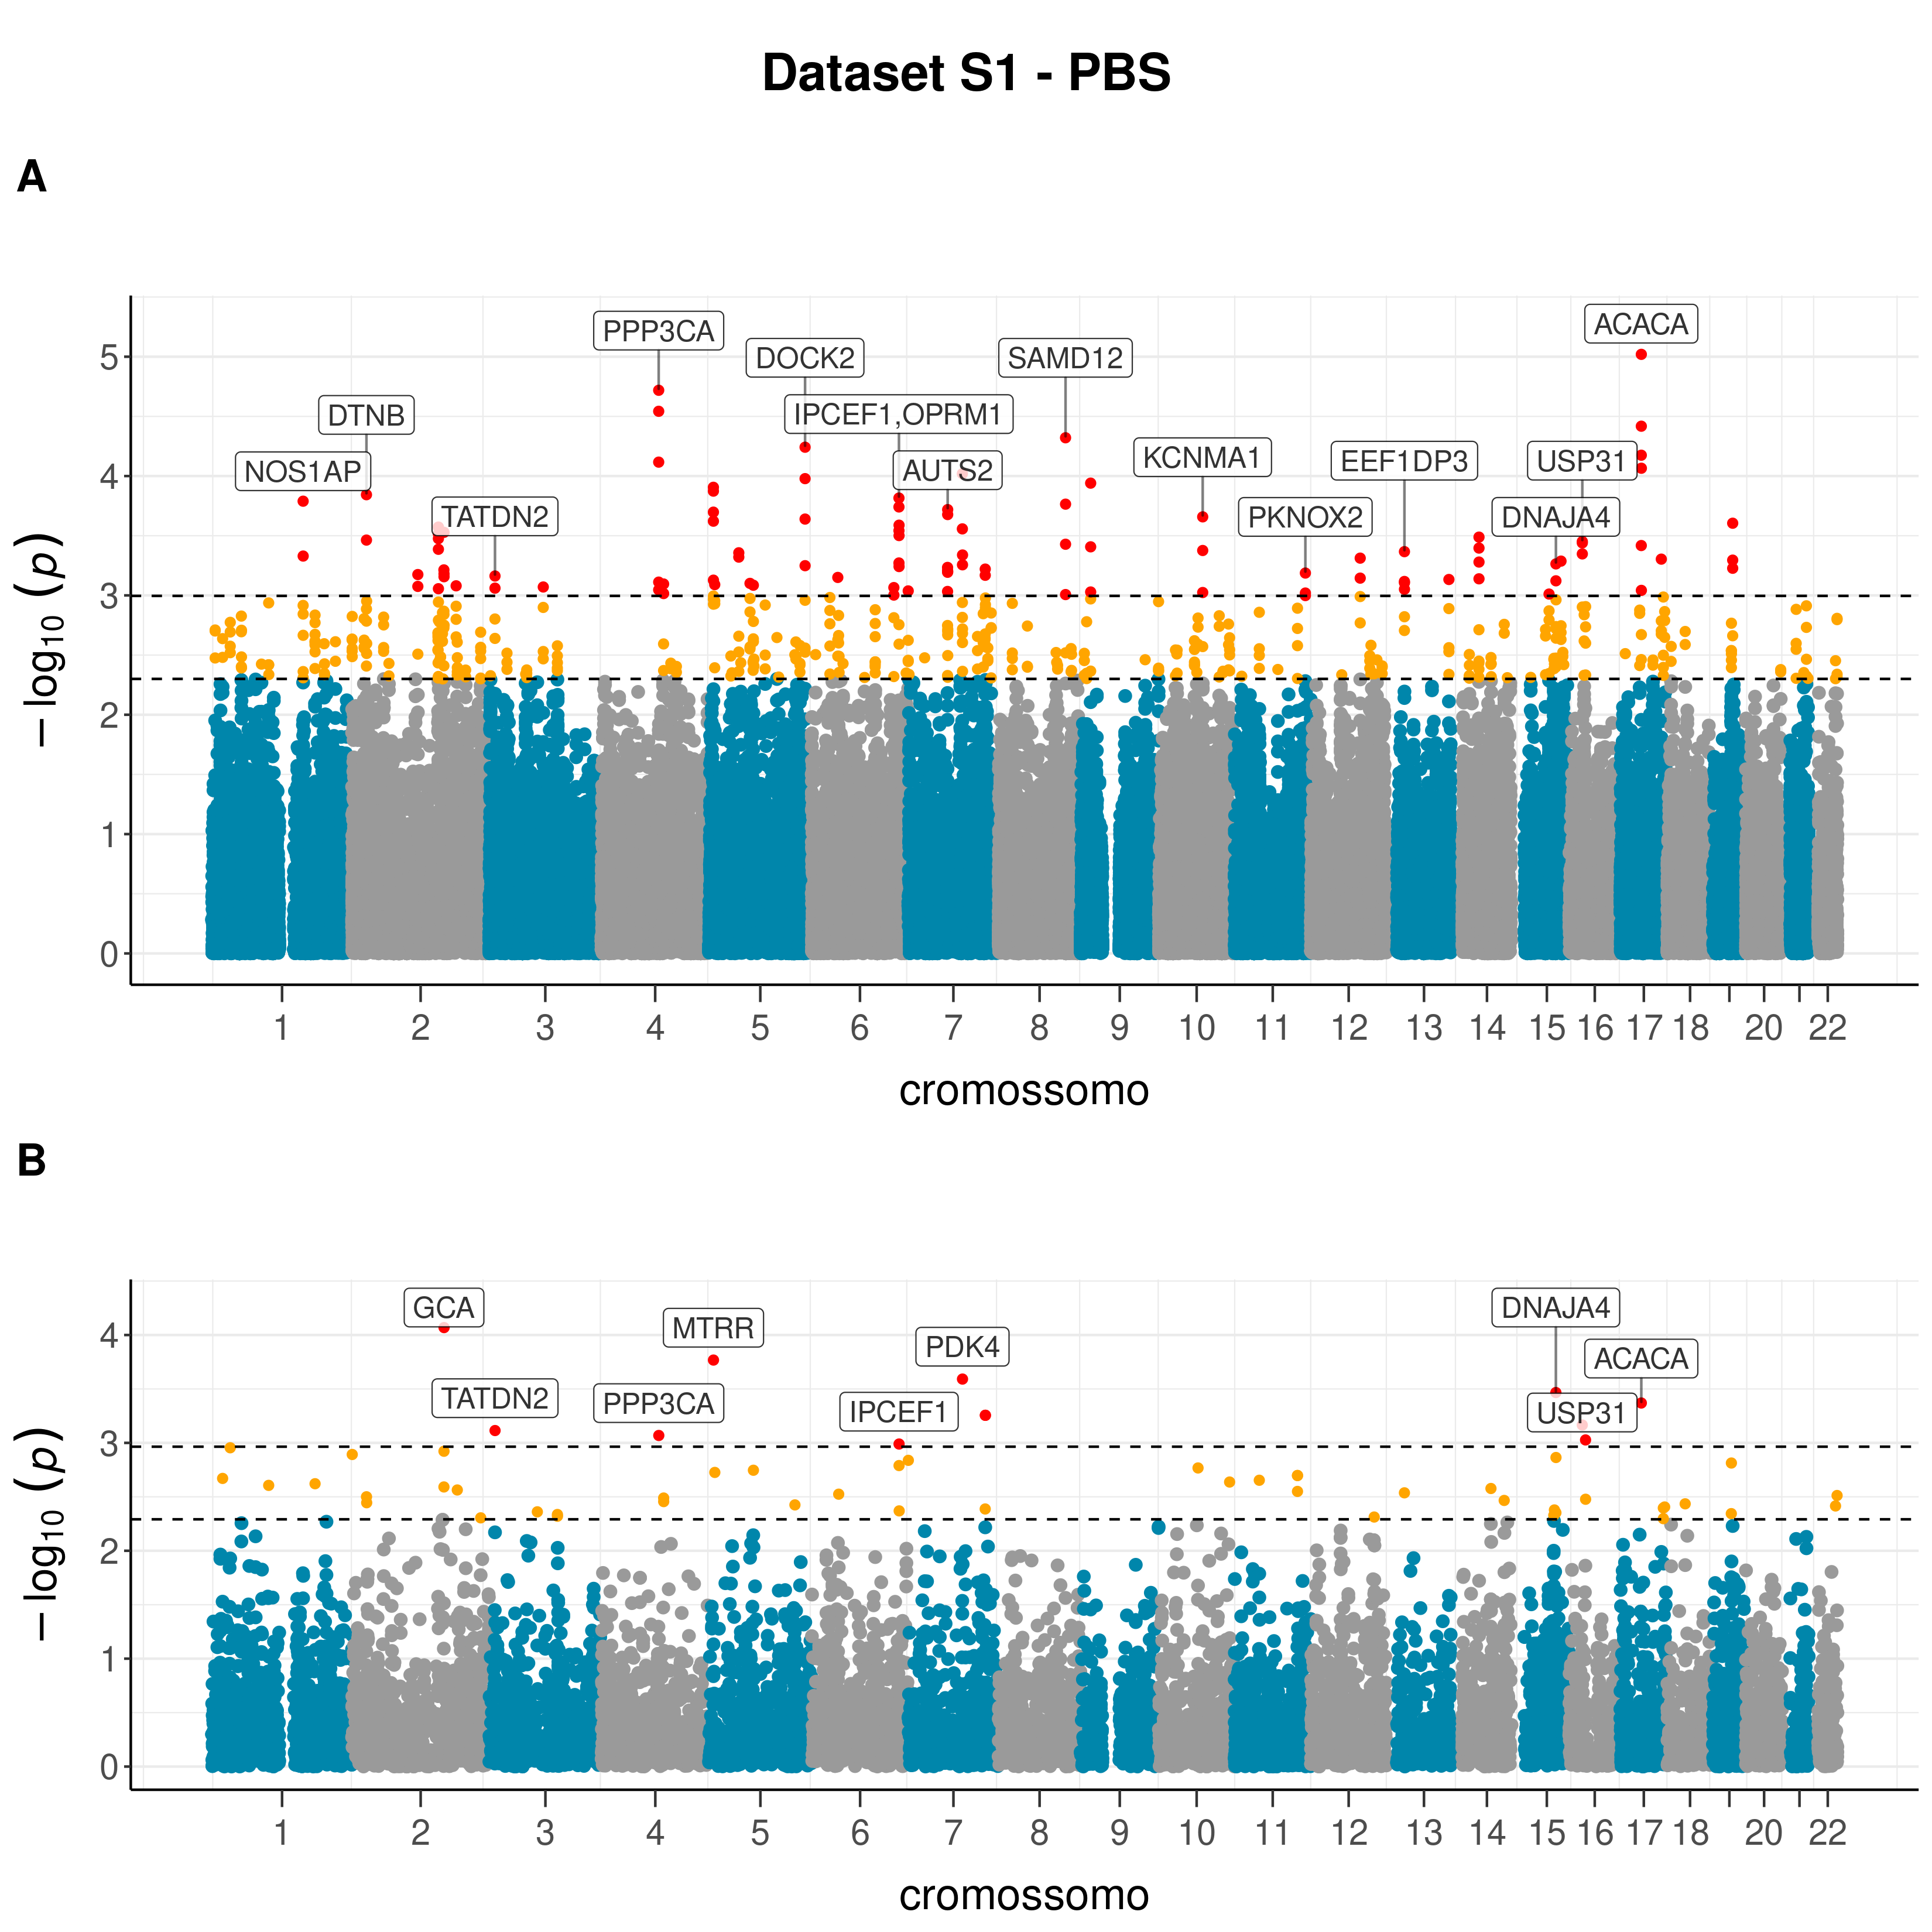
\includegraphics[width=1.0\linewidth]{ds1_pbsw_both}
    \caption[Resultados da análise de PBS para o dataset S1.]{Resultados da análise de PBS para o dataset S1. (A) Abordagem por SNP. (B) Abordagem por gene. Na abordagem por SNP cada ponto corresponde ao SNP com o valor mais alto dentro da média móvel de PBS. Na abordagem por gene cada ponto representa a média dos valores de PBS de todos SNPs para cada gene. As linhas horizontais pontilhadas representam os quantis 0,995 e 0,999, enquanto as cores laranja e vermelha denotam os (A) SNPs e (B) genes distribuídos acima destes quantis, respectivamente. Para cada cromossomo, (A) apontamos os genes correspondentes ao SNP com o valor mais alto na abordagem por SNP e (B) reportamos diretamente o gene com maior valor de PBS, considerando em ambos os casos apenas os pontos com valores iguais ou superiores ao quantil 0.999.}
    \label{fig:ds1_pbsw_both}
\end{figure}

\begin{table}[!htbp]
\centering
\resizebox{\linewidth}{!}{
\begin{tabular}[t]{crlllrr}
\toprule
CHR & POS & SNP & GENE & FUNÇÃO & PBS & -log$_{10}(p)$\\
\midrule
1 & 32686594 & rs3738001 & TMEM234 & intronic & 0.2227 & 3.3645\\
1 & 47571391 & rs6690005 & CYP4Z1 & intronic & 0.1862 & 3.0366\\
2 & 85115111 & rs6728804 & TRABD2A & intergenic & 0.1958 & 3.1228\\
5 & 71744199 & rs10068109 & ZNF366 & intronic & 0.1936 & 3.0921\\
5 & 160134369 & rs2033462 & ATP10B & intronic & 0.2160 & 3.2884\\
7 & 95216262 & rs4729201 & PDK4 & intronic & 0.2486 & 3.6217\\
7 & 132094453 & rs2341825 & PLXNA4 & intronic & 0.3609 & 4.7356\\
8 & 24339679 & rs13255694 & ADAM7 & exonic & 0.2060 & 3.2171\\
9 & 17801555 & rs11791520 & SH3GL2 & intergenic & 0.2384 & 3.5595\\
10 & 22504189 & rs2148959 & EBLN1 & intergenic & 0.2099 & 3.2373\\
10 & 61801739 & rs10821662 & ANK3 & intronic & 0.2325 & 3.4568\\
10 & 102689217 & rs2273654 & SLF2 & intronic & 0.1939 & 3.0971\\
11 & 118825636 & rs1790191 & UPK2 & intergenic & 0.1849 & 3.0196\\
12 & 111614736 & rs6489979 & CUX2 & intronic & 0.2853 & 3.8605\\
12 & 112233018 & rs10744777 & ALDH2 & intronic & 0.3860 & 5.0366\\
12 & 112463296 & rs4767293 & ERP29,NAA25 & intergenic,intergenic & 0.1916 & 3.0681\\
12 & 112667675 & rs1005902 & HECTD4 & exonic & 0.2924 & 3.9952\\
12 & 114254860 & rs1043811 & RBM19 & UTR3 & 0.1830 & 3.0032\\
13 & 24525604 & rs2147995 & ANKRD20A19P & intergenic & 0.2022 & 3.1854\\
13 & 74532811 & rs1570744 & KLF12 & intronic & 0.2049 & 3.2106\\
14 & 103427555 & rs10136828 & CDC42BPB & intronic & 0.2151 & 3.2808\\
15 & 65626219 & rs894491 & IGDCC3 & intronic & 0.1856 & 3.0238\\
15 & 75242155 & rs2415251 & RPP25 & intergenic & 0.1861 & 3.0323\\
16 & 28922149 & rs11646653 & RABEP2 & intronic & 0.2636 & 3.7579\\
19 & 49399821 & rs12461075 & TULP2 & intronic & 0.2454 & 3.5895\\
\bottomrule
\end{tabular}}

\caption{Resultado da análise de PBS por SNP no dataset S2.}
\label{tab:ds2_pbsw_persnp}

\end{table}
 % tabela 2.6

\begin{figure}[!htbp] % figura 2.5
    \centering
    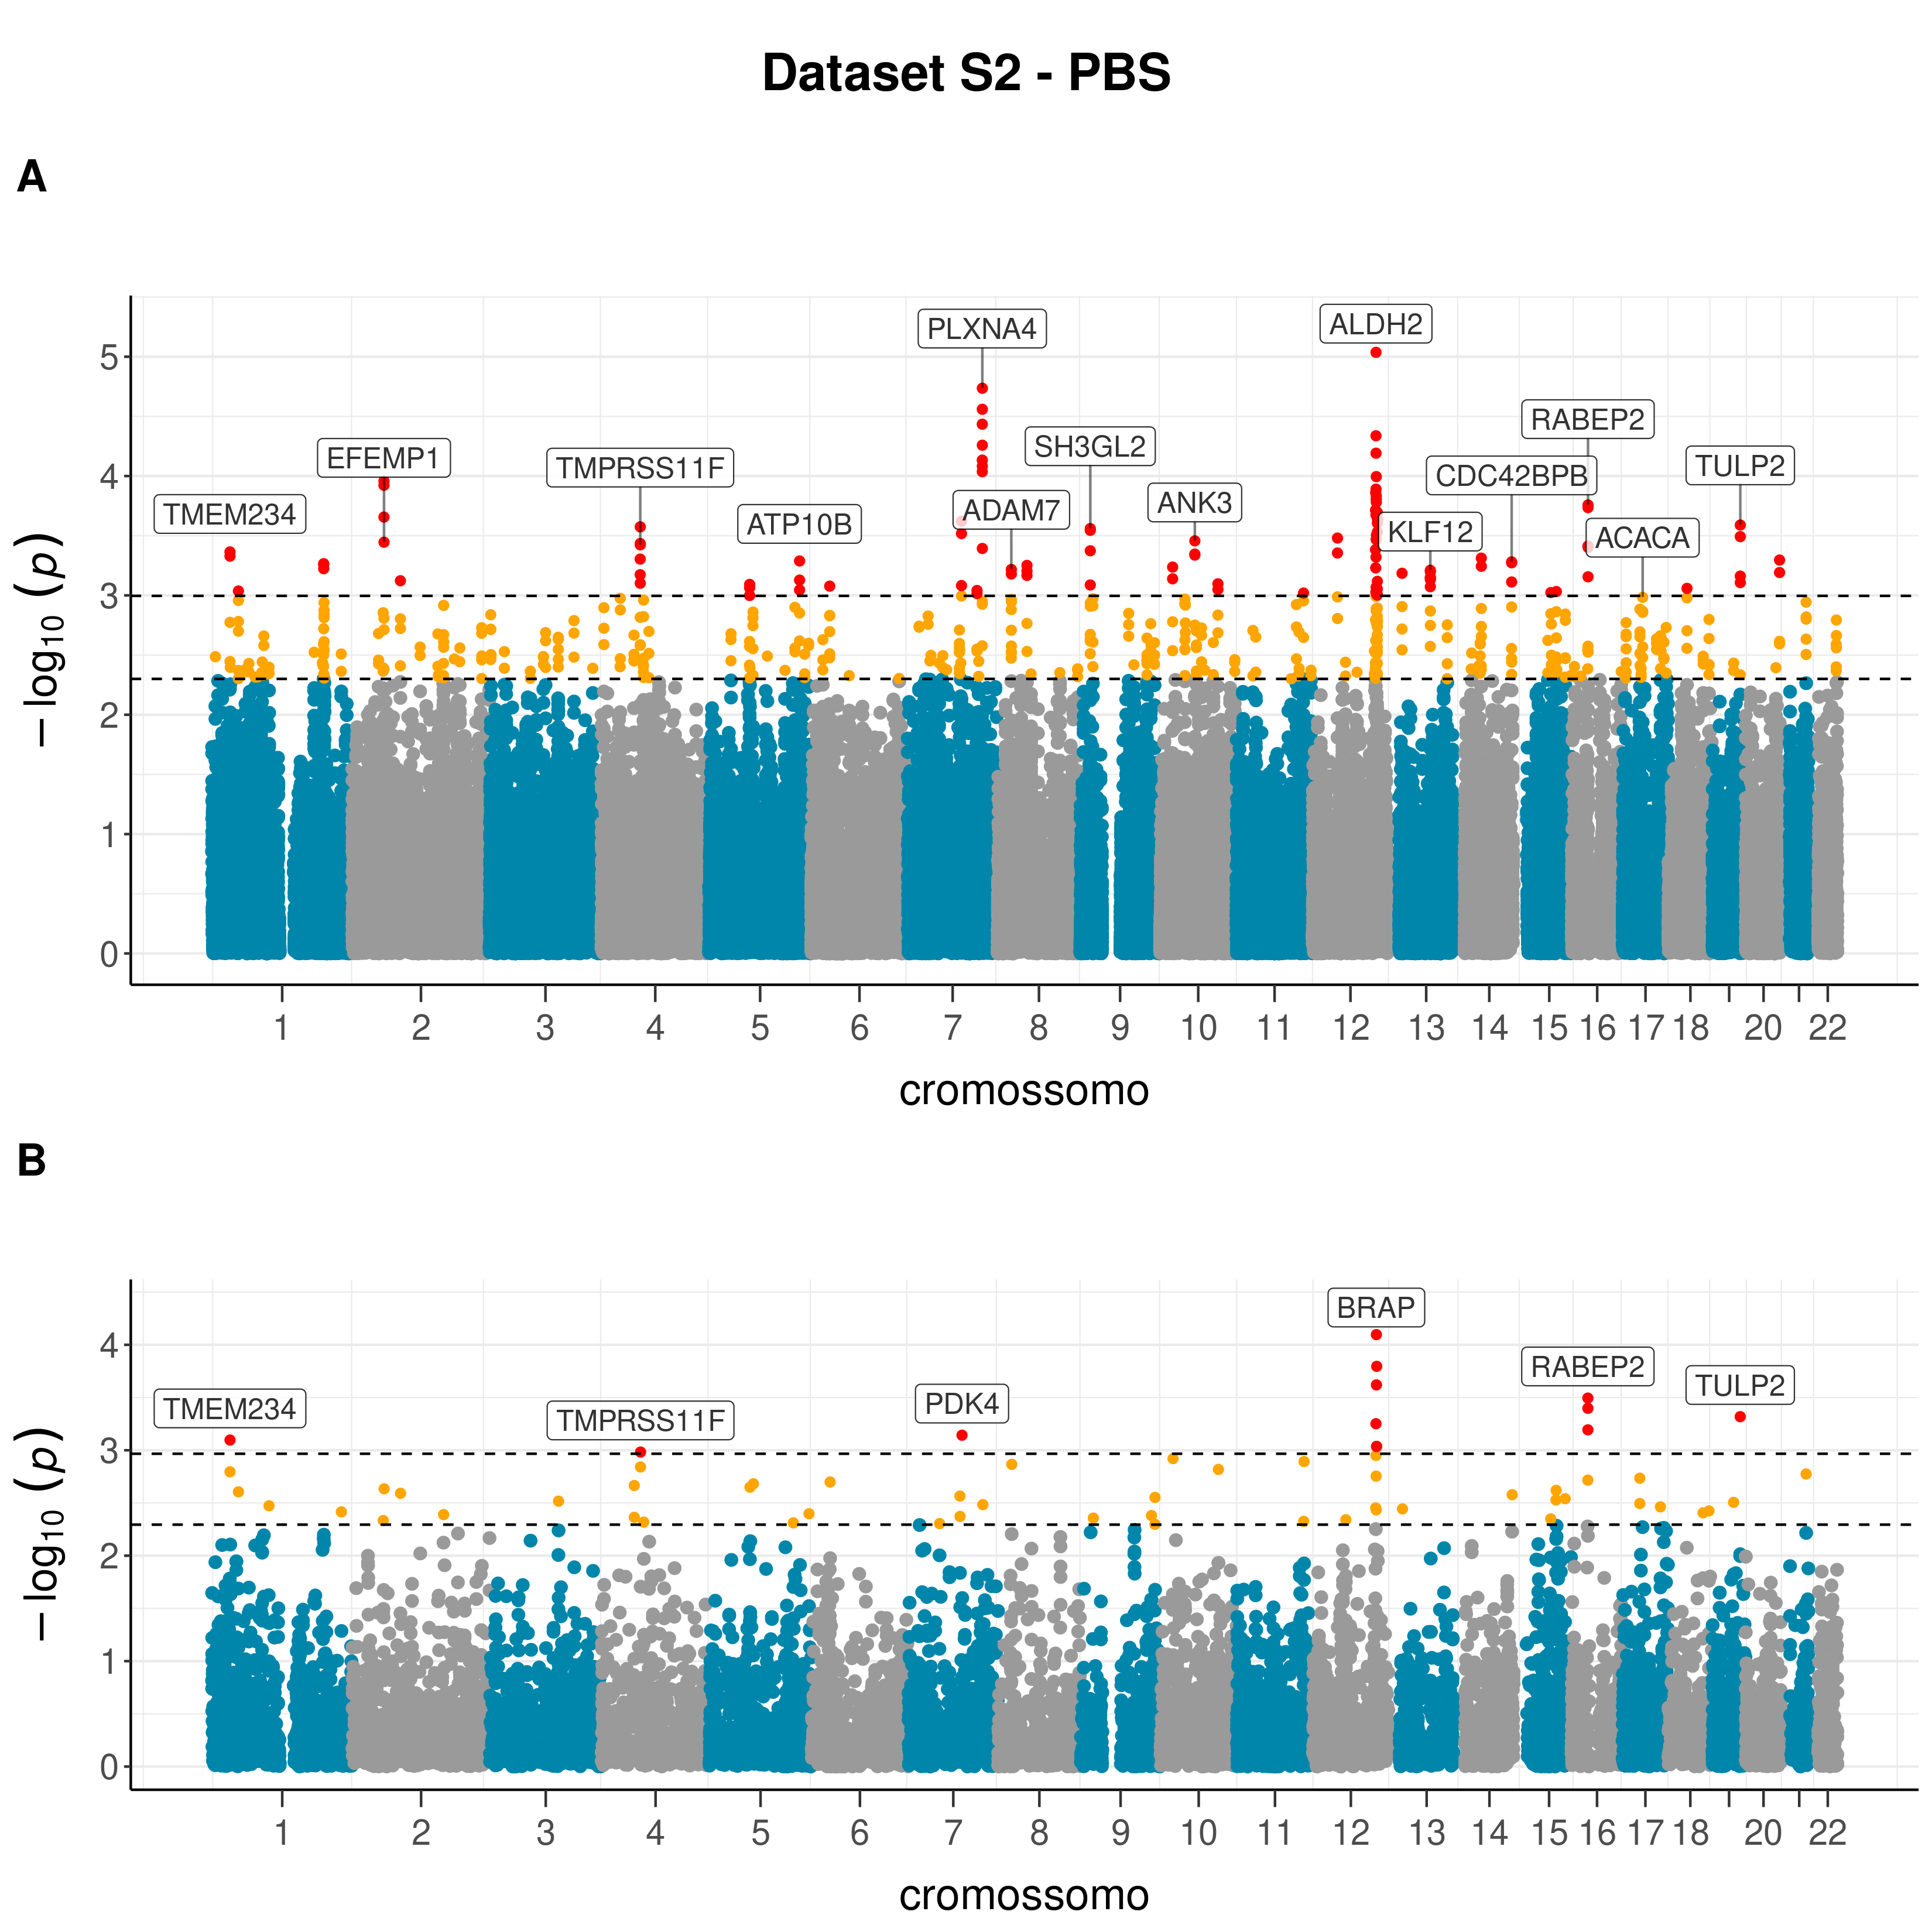
\includegraphics[width=1.0\linewidth]{ds2_pbsw_both}
    \caption[Resultados da análise de PBS para o dataset S2.]{Resultados da análise de PBS para o dataset S2. (A) Abordagem por SNP. (B) Abordagem por gene. Na abordagem por SNP cada ponto corresponde ao SNP com o valor mais alto dentro da média móvel de PBS. Na abordagem por gene cada ponto representa a média dos valores de PBS de todos SNPs para cada gene. As linhas horizontais pontilhadas representam os quantis 0,995 e 0,999, enquanto as cores laranja e vermelha denotam os (A) SNPs e (B) genes distribuídos acima destes quantis, respectivamente. Para cada cromossomo, (A) apontamos os genes correspondentes ao SNP com o valor mais alto na abordagem por SNP e (B) reportamos diretamente o gene com maior valor de PBS, considerando em ambos os casos apenas os pontos com valores iguais ou superiores ao quantil 0.999.}
    \label{fig:ds2_pbsw_both}
\end{figure}

\begin{table}[!htbp]
\centering

\begin{tabular}[!htbp]{
    >{\centering\arraybackslash}p{2.5cm}
    >{\raggedleft\arraybackslash}p{1cm}
    >{\raggedright\arraybackslash}p{2.5cm}
    >{\raggedleft\arraybackslash}p{2cm}
    >{\raggedleft\arraybackslash}p{2cm}
    %lrlrr % crlrr
}

\toprule
DATASET & CHR & GENE & PBS & -log$_{10}(p)$\\
\rowcolor{gray!6}
\midrule
 & 2 & GCA & 0.2060 & 4.0687\\
\rowcolor{gray!6}
 & 3 & TATDN2 & 0.1636 & 3.1144\\
\rowcolor{gray!6}
 & 4 & PPP3CA & 0.1623 & 3.0687\\
\rowcolor{gray!6}
 & 5 & MTRR & 0.2021 & 3.7676\\
\rowcolor{gray!6}
 & 6 & IPCEF1 & 0.1485 & 2.9895\\
\rowcolor{gray!6}
 & 7 & PDK4 & 0.2005 & 3.5915\\
\rowcolor{gray!6}
 & 7 & LUZP6,MTPN & 0.1667 & 3.2558\\
\rowcolor{gray!6}
 & 15 & DNAJA4 & 0.1719 & 3.4666\\
\rowcolor{gray!6}
 & 16 & USP31 & 0.1658 & 3.1656\\
\rowcolor{gray!6}
 & 16 & ATXN2L & 0.1609 & 3.0273\\
\rowcolor{gray!6}

\multirow{-11}{*}{\raggedright\arraybackslash Dataset S1} & 17 & ACACA & 0.1713 & 3.3697\\
\midrule
%\cmidrule{1-5}
 & 1 & TMEM234 & 0.1942 & 3.0968\\
 & 4 & TMPRSS11F & 0.1916 & 2.9828\\
 & 7 & PDK4 & 0.1953 & 3.1425\\
 & 12 & LINC01405 & 0.2163 & 3.2517\\
 & 12 & BRAP & 0.2925 & 4.0968\\
 & 12 & ALDH2 & 0.2781 & 3.6196\\
 & 12 & ERP29,NAA25 & 0.1934 & 3.0361\\
 & 12 & HECTD4 & 0.2821 & 3.7957\\
 & 16 & RABEP2 & 0.2621 & 3.4947\\
 & 16 & NFATC2IP & 0.2270 & 3.3978\\
 & 16 & SPNS1 & 0.1980 & 3.1937\\
\multirow{-12}{*}{\raggedright\arraybackslash Dataset S2} & 19 & TULP2 & 0.2182 & 3.3186\\
\bottomrule
\end{tabular}

\caption{Resultado da análise de PBS por gene nos datasets S1 e S2.}
\label{tab:pbsw_pergene}

\end{table}
 % tabela 2.7

\begin{figure}[!htbp] % figura 2.6
    \centering
    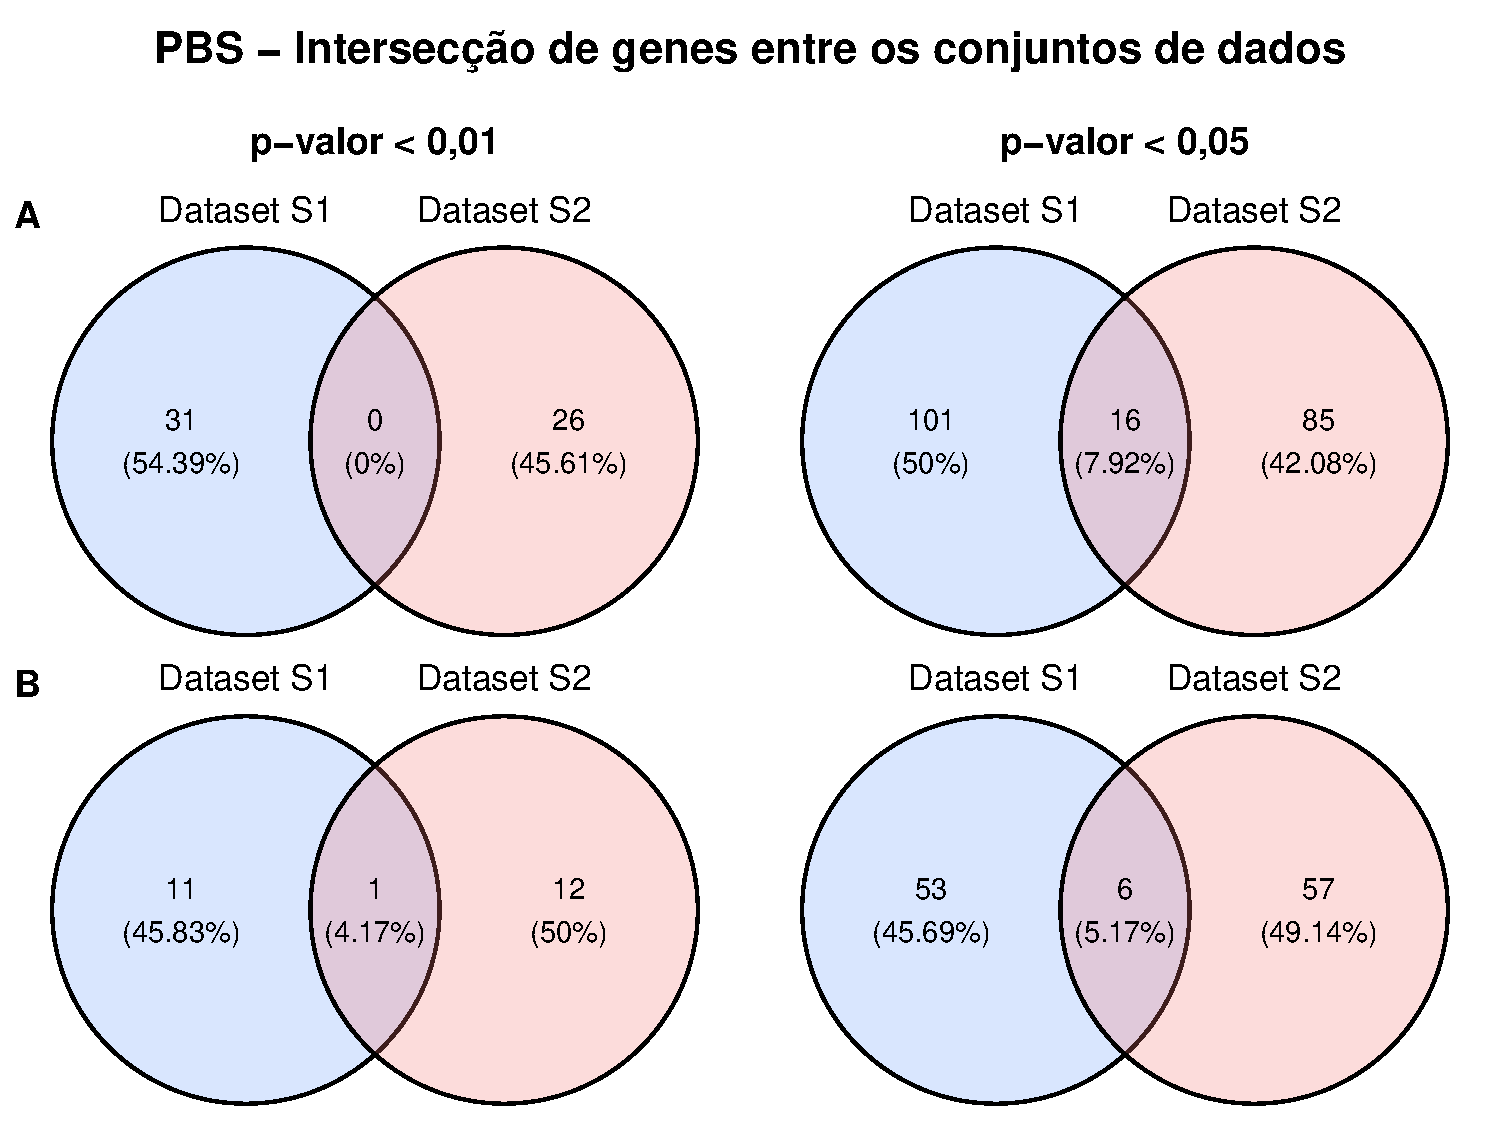
\includegraphics[width=1.0\linewidth]{pbs_intersection}
    \caption[Intersecção dos genes candidatos na análise de PBS entre os datasets]{Intersecção dos genes candidatos na análise de PBS entre os datasets. (A) Abordagem por SNP. (B) Abordagem por gene. Os genes foram identificados utilizando como valores de corte os SNPs/genes com \emph{p}-valor abaixo de 0,01 e 0,05 (colunas 1 e 2), respectivamente.}
    \label{fig:pbs_intersection}
\end{figure}

Nas análises derivadas da estatística de EHH, selecionamos os SNPs com \emph{p}-valores empíricos menores que 0,001 para os  métodos XP-EHH e iHS, que por sua vez mapearam para 59 e 70 genes no dataset S1, respectivamente (tabelas disponíveis no repositório Mendeley). De forma similar à análise de PBS, calculamos a média por gene para cada uma destas estatísticas, resultando em 21 e 17 genes. Os genes mais representativos no método XP-EHH estão representados na figura \ref{fig:ds1_xpehh_both}, ao passo que os resultados do método iHS podem ser verificados no repositório Mendeley.

\begin{figure}[!htbp] % figura 2.7
    \centering
    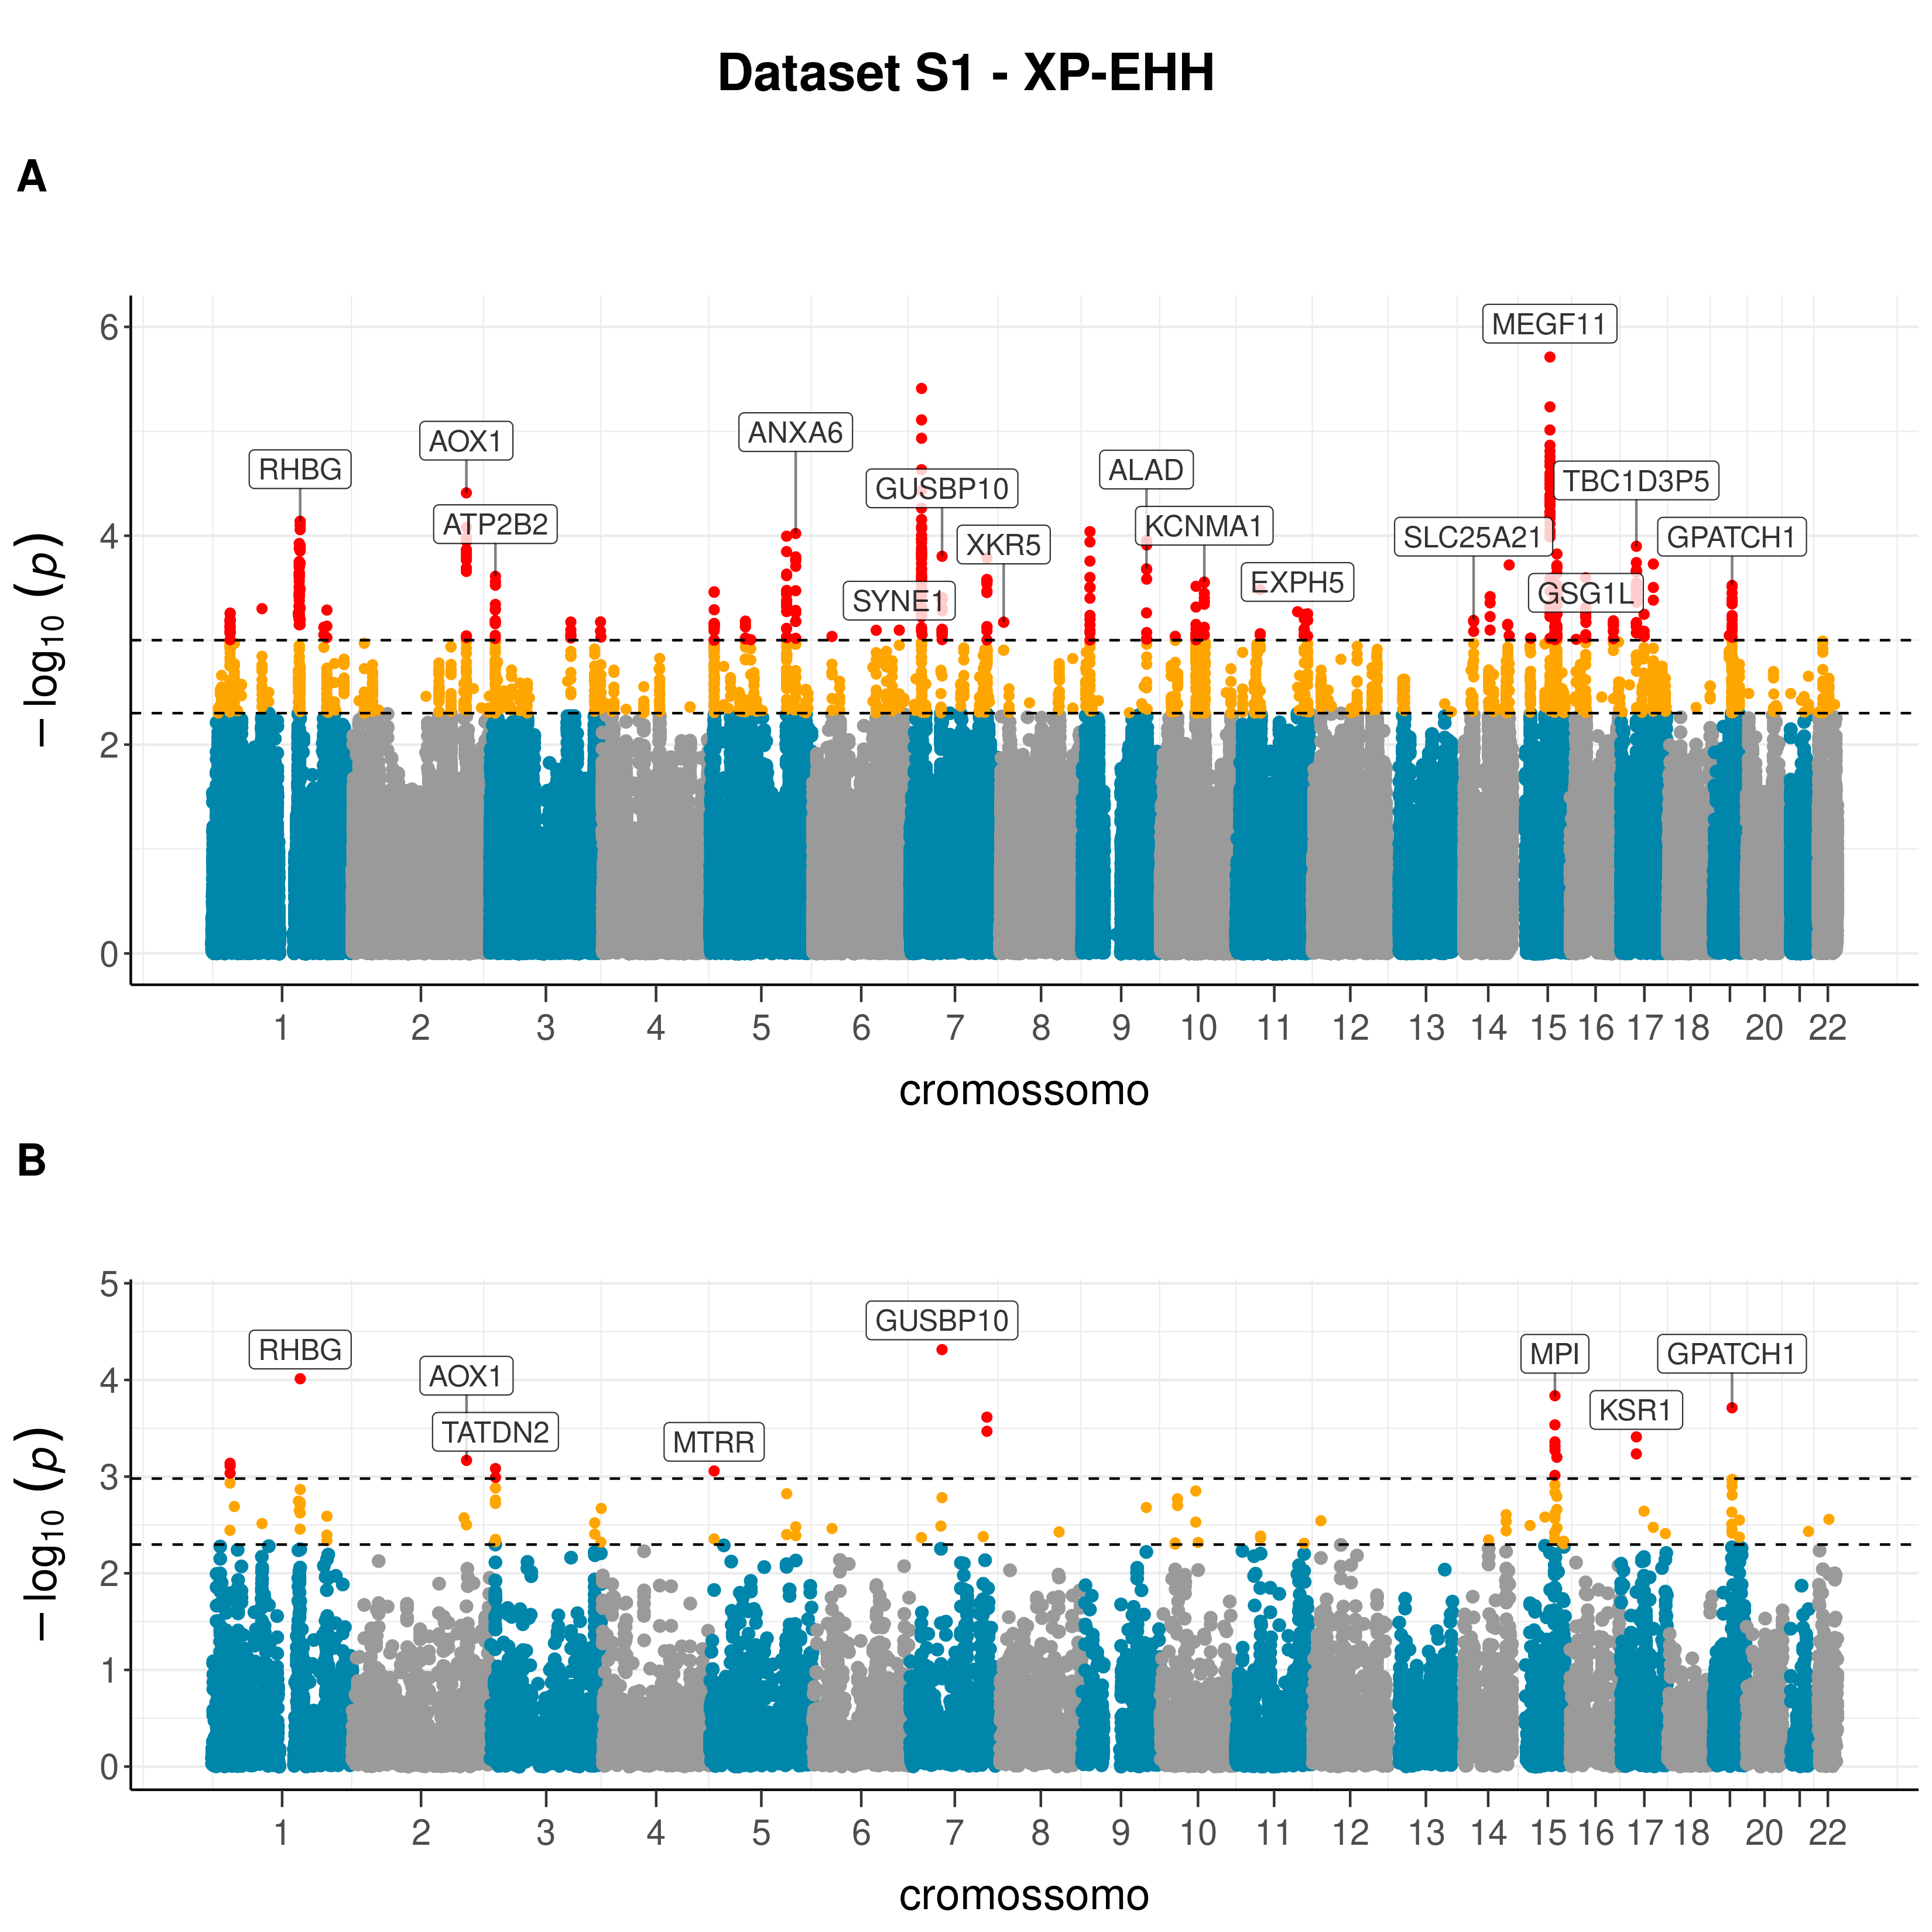
\includegraphics[width=1.0\linewidth]{ds1_xpehh_both}
    \caption[Resultados da análise de XP-EHH para o dataset S1.]{Resultados da análise de XP-EHH para o dataset S1. (A) Abordagem por SNP. (B) Abordagem por gene. As linhas horizontais pontilhadas representam os quantis 0,995 e 0,999, enquanto as cores laranja e vermelha denotam os (A) SNPs e (B) genes distribuídos acima destes quantis, respectivamente. Para cada cromossomo, (A) apontamos os genes correspondentes ao SNP com o valor mais alto na abordagem por SNP e (B) reportamos diretamente o gene com maior valor de XP-EHH, considerando em ambos os casos apenas os pontos com valores iguais ou superiores ao quantil 0.999. Nota-se um acentuado valor no cromossomo 15 na abordagem por SNP, mapeando para o gene \textsl{MEGF11}. Os SNPs com valores acentuados no cromossomo 7 não mapeiam para nenhum gene ao redor de 10kb dos mesmos.}
    \label{fig:ds1_xpehh_both}
\end{figure}

Aplicando os mesmos métodos no segundo conjunto de dados (\emph{i.e.} XP-EHH e iHS), identificamos 54 e 135 genes na abordagem de \textsl{outliers} por SNP, e 22 e 21 genes na abordagem de genes \textsl{outliers} por gene, respectivamente. A figura \ref{fig:ds2_xpehh_both} apresenta os \textsl{outliers} em ambas as abordagens para o método XP-EHH, enquanto as tabelas para ambos os métodos e as figuras para o método iHS podem ser acessadas via repositório Mendeley.

\begin{figure}[!htbp] % figura 2.8
    \centering
    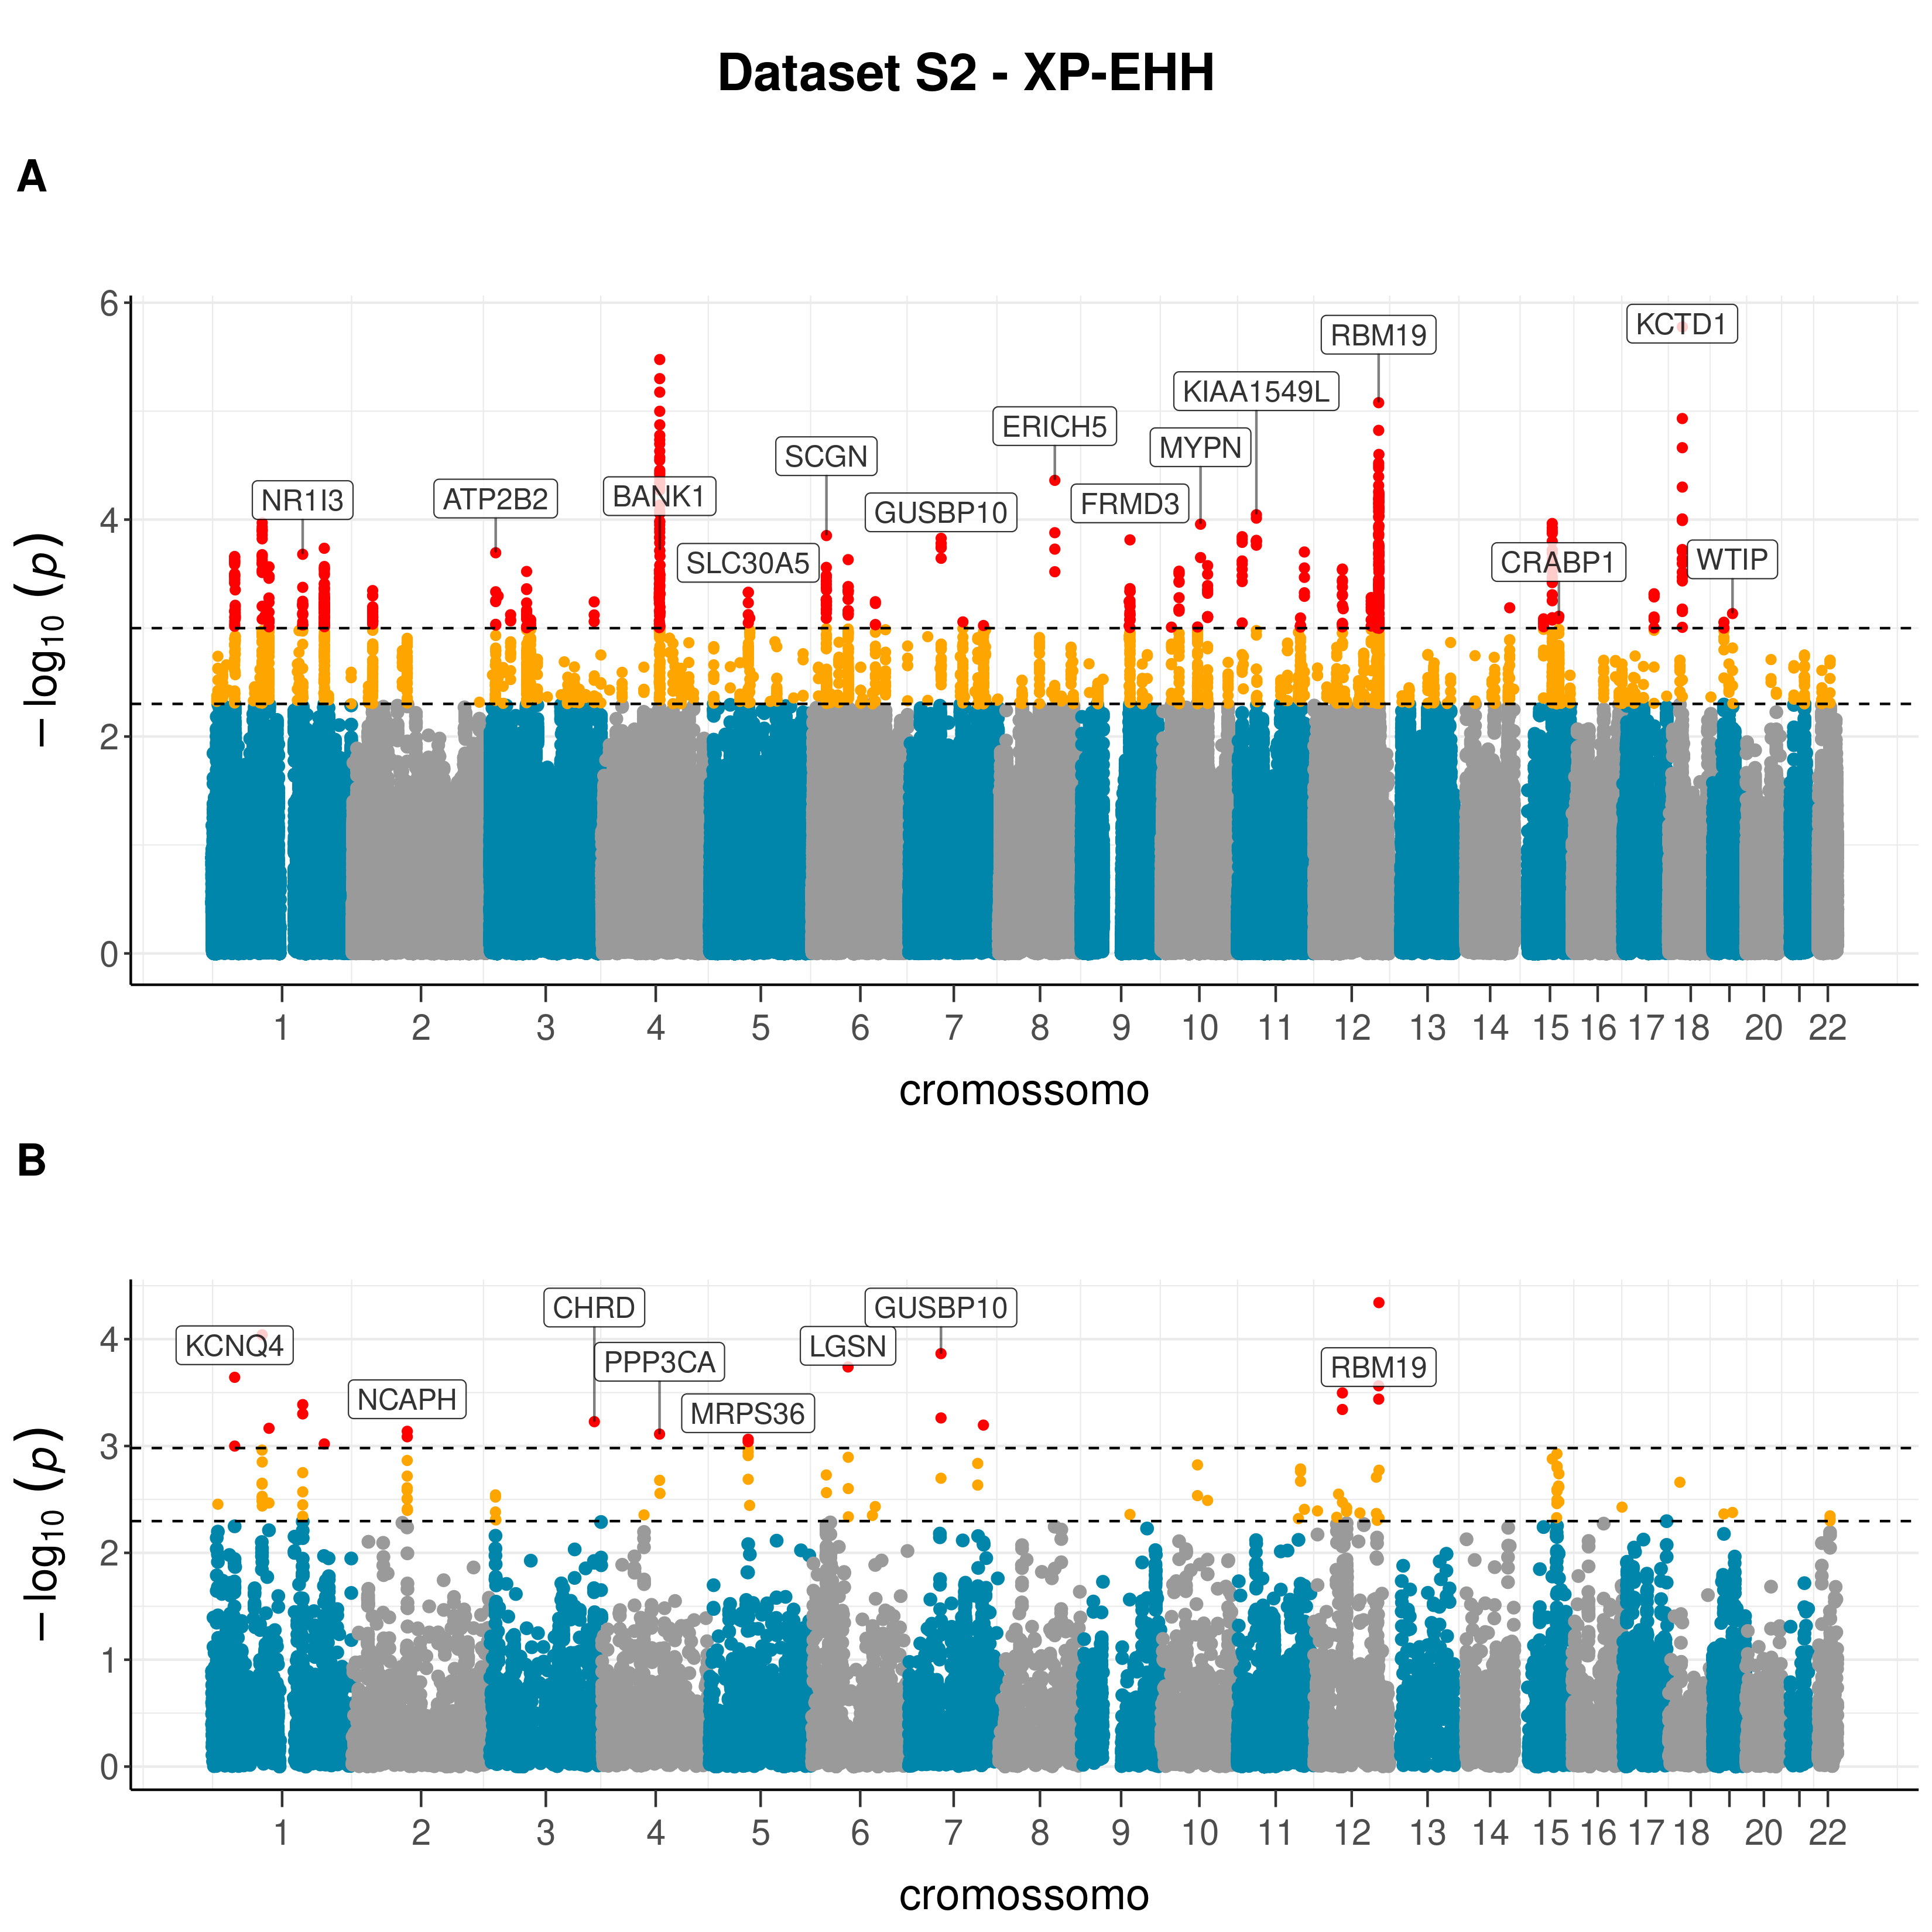
\includegraphics[width=1.0\linewidth]{ds2_xpehh_both}
    \caption[Resultados da análise de XP-EHH para o dataset S2.]{Resultados da análise de XP-EHH para o dataset S2. (A) Abordagem por SNP. (B) Abordagem por gene. As linhas horizontais pontilhadas representam os quantis 0,995 e 0,999, enquanto as cores laranja e vermelha denotam os (A) SNPs e (B) genes distribuídos acima destes quantis, respectivamente. Para cada cromossomo, (A) apontamos os genes correspondentes ao SNP com o valor mais alto na abordagem por SNP e (B) reportamos diretamente o gene com maior valor de XP-EHH, considerando em ambos os casos apenas os pontos com valores iguais ou superiores ao quantil 0.999. Os SNPs com valores mais acentuados no cromossomo 4, na abordagem por SNP, não mapeiam para nenhum gene ao redor de 10kb dos mesmos.}
    \label{fig:ds2_xpehh_both}
\end{figure}

Pode-se observar que, na abordagem tradicional por SNP, mais genes são mapeados no método iHS em ambos os datasets, quando comparado às estatísticas XP-EHH e PBS (Figuras \ref{fig:ds1_intersection}-\ref{fig:ds2_intersection}). Logo, verificamos a distribuição dos valores nestes métodos, em ambos os datasets, apresentados nas Figuras \ref{fig:ds1_density} e \ref{fig:ds2_density}, respectivamente.

\begin{figure}[p] % figura 2.9
    \centering
    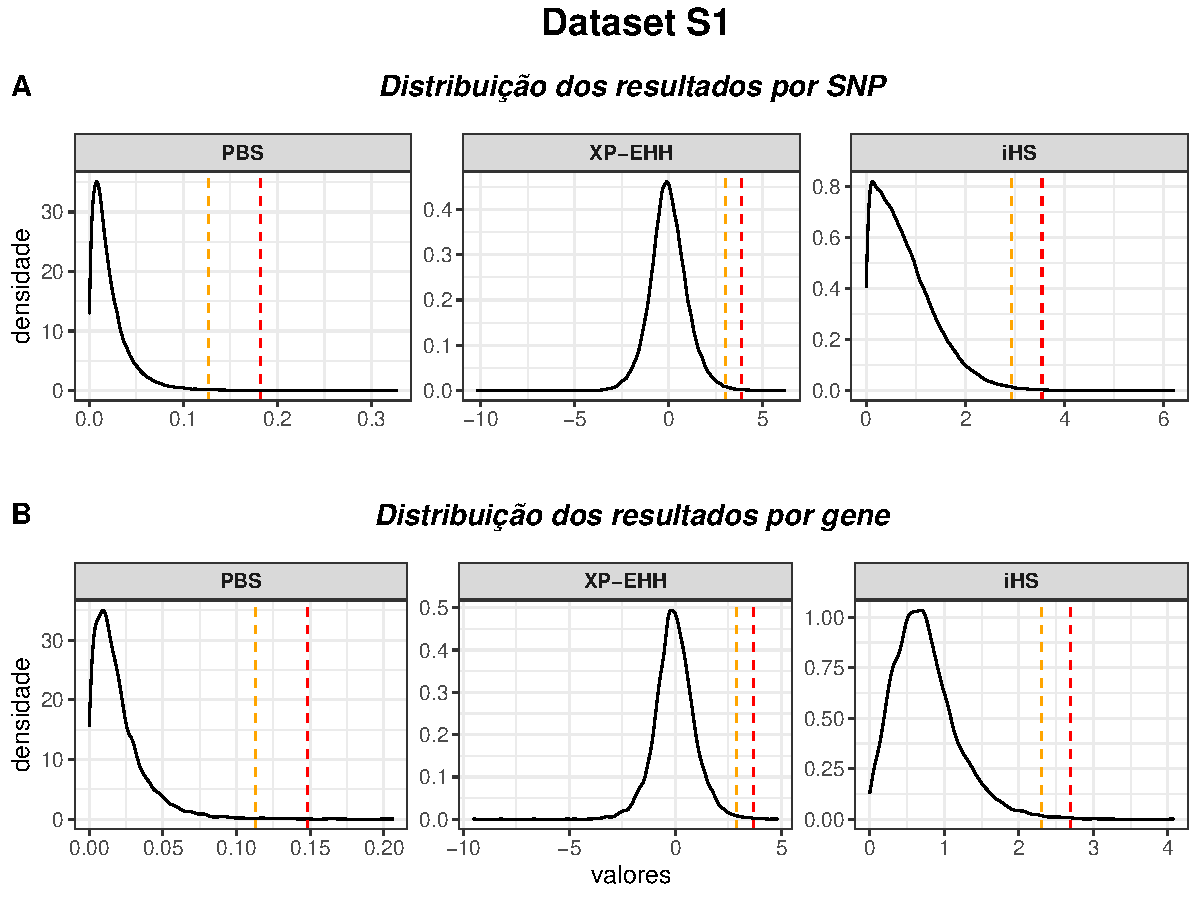
\includegraphics[width=.85\linewidth]{ds1_density}
    \caption[Distribuição dos valores dos testes de seleção no Dataset S1.]{Distribuição dos valores dos testes de seleção no Dataset S1. (A) Abordagem por SNP. (B) Abordagem por gene. As linhas verticais amarelas e vermelhas representam os quantis 0.995 e 0.999, respectivamente.}
    \label{fig:ds1_density}
\end{figure}

\begin{figure}[p] % figura 2.10
    \centering
    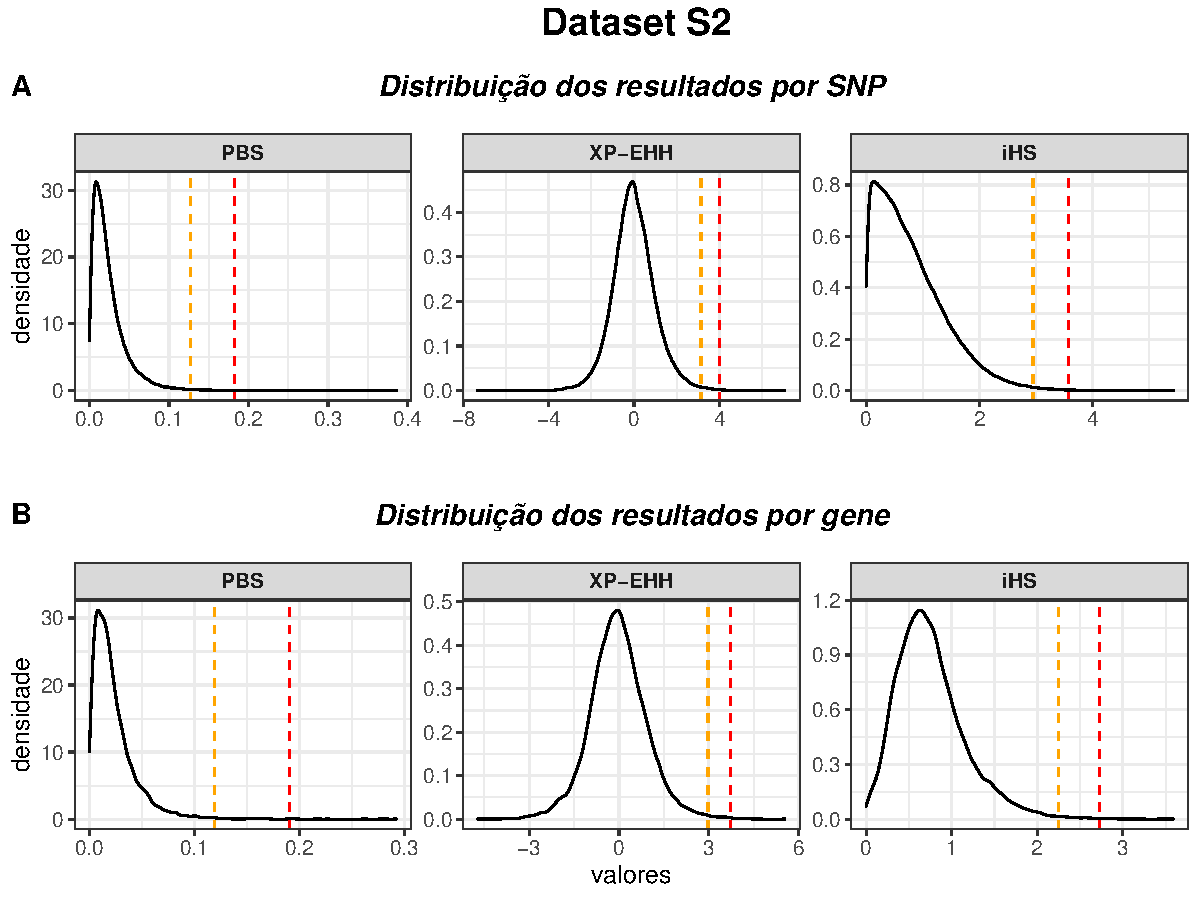
\includegraphics[width=.85\linewidth]{ds2_density}
    \caption[Distribuição dos valores dos testes de seleção no Dataset S2.]{Distribuição dos valores dos testes de seleção no Dataset S2. (A) Abordagem por SNP. (B) Abordagem por gene. As linhas verticais amarelas e vermelhas representam os quantis 0.995 e 0.999, respectivamente.}
    \label{fig:ds2_density}
\end{figure}

\begin{figure}[!htbp] % figura 2.11
    \centering
    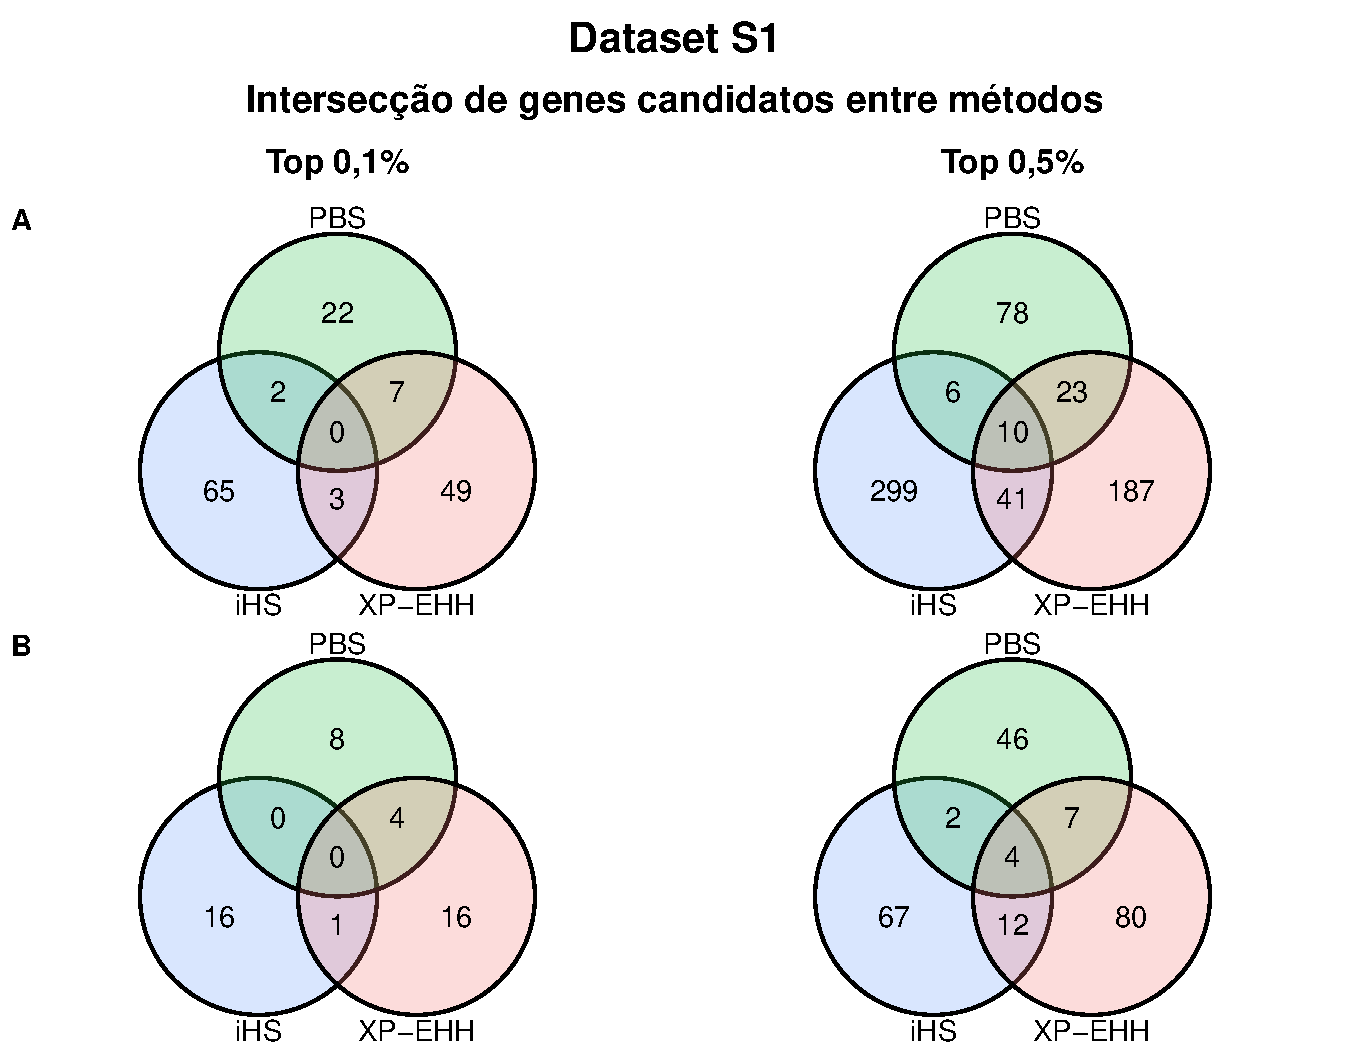
\includegraphics[width=1.0\linewidth]{ds1_intersection}
    \caption[Intersecção dos genes candidatos no dataset S1.]{Intersecção dos genes candidatos no dataset S1. (A) Abordagem por SNP. (B) Abordagem por gene. No painel esquerdo foi considerado o extremo 0,1\% da distribuição das estatísticas para identificação dos genes candidatos, ao passo que, no painel direito, 0,5\%.}
    \label{fig:ds1_intersection}
\end{figure}

\begin{figure}[!htbp] % figura 2.12
    \centering
    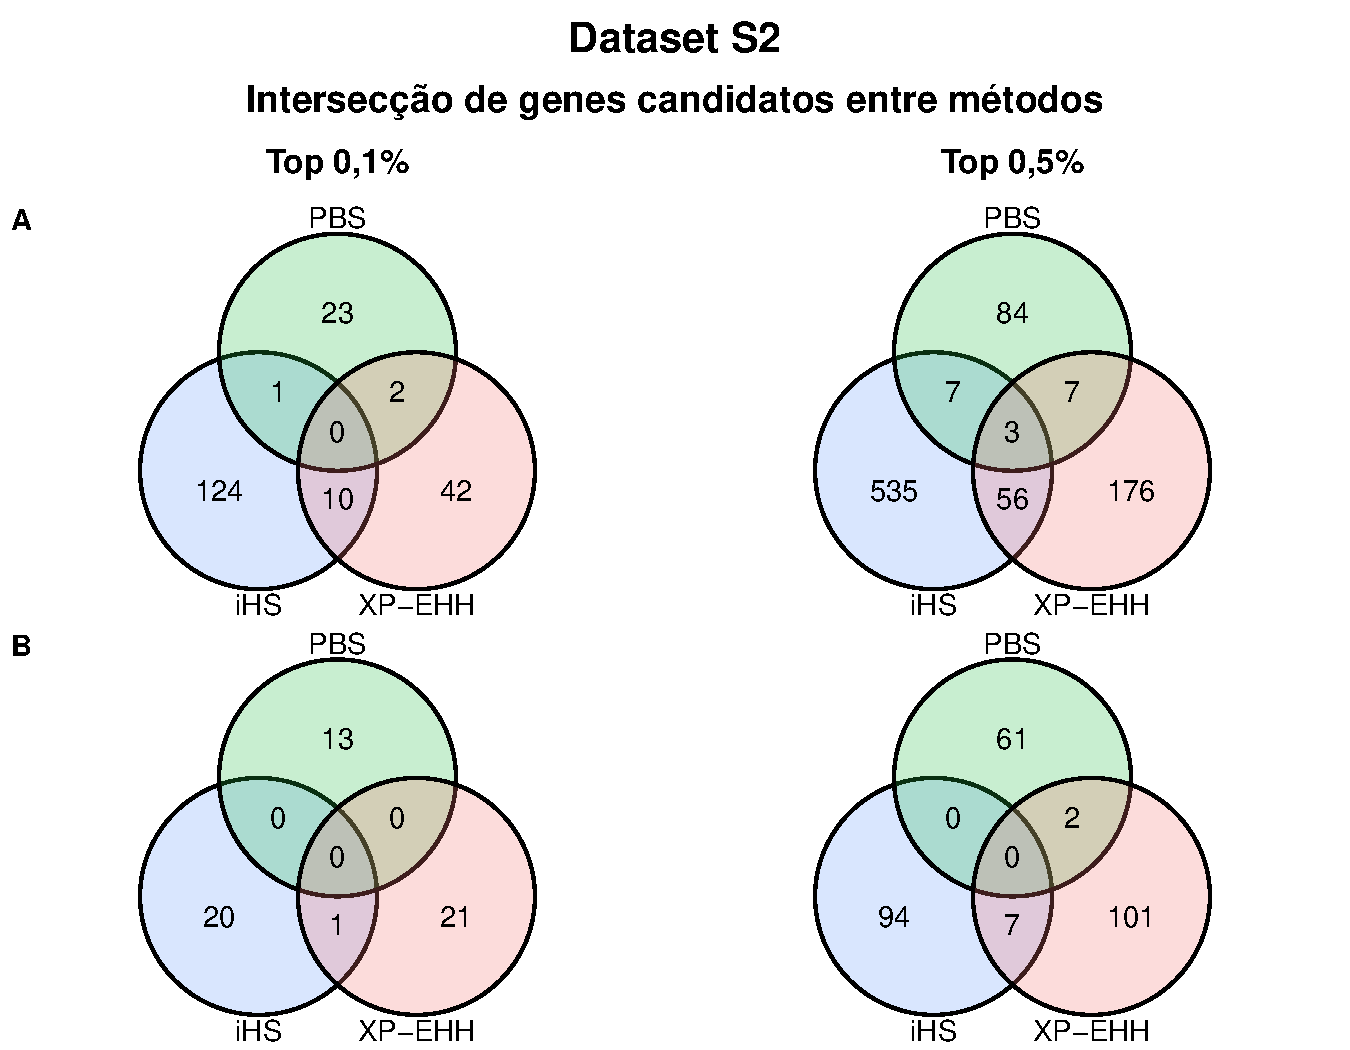
\includegraphics[width=1.0\linewidth]{ds2_intersection}
    \caption[Intersecção dos genes candidatos no dataset S2.]{Intersecção dos genes candidatos no dataset S1. (A) Abordagem por SNP. (B) Abordagem por gene. No painel esquerdo foi considerado o extremo 0,1\% da distribuição das estatísticas para identificação dos genes candidatos, ao passo que, no painel direito, 0,5\%.}
    \label{fig:ds2_intersection}
\end{figure}

\clearpage
\subsection{Anotação Funcional}
\label{subsec:amazonia_results_annotfuncional}

Para compreender melhor os fenótipos resultantes dos genes levantados pelas análises de seleção acima apontadas, buscamos os fenótipos associados aos mesmos em dois bancos de dados públicos: Ensembl e GWAS Catalog. As tabelas \ref{tab:ds1_gwas_persnp}-\ref{tab:ds2_gwas_pergene} contém os resultados destas da abordagem por SNP nos dois datasets analisados. Nestas tabelas, ordenamos os fenótipos primeiramente pela quantidade de genes candidatos mapeados para os mesmos (colunas “N”), e então por ordem alfabética, restringindo cada tabela aos trinta primeiros fenótipos.

Adicionalmente, verificamos também a expressão dos alelos candidatos provenientes das análises de PBS e XP-EHH (\emph{p}-valor < 0,01). Para cada SNP, definimos como alelo-alvo aquele com maior frequência na população amazônica quando comparado à Mesoamérica, e buscamos no banco de dados GTEx sua influência na expressão dos seus respectivos genes, mantendo apenas os alelos cujo eQTL possui \emph{p}-valor menor que 0,01 no tecido (Figuras \ref{fig:overall_eqtl_score} e \ref{fig:overall_eqtl_count}). Reportamos aqui a contagem dos alelos com eQTL significativo considerando ambos os métodos e datasets em conjunto, ao passo que as figuras separadas e as tabelas completas podem ser verificadas no repositório Mendeley.

\begin{landscape}
\begin{table}[hp]
\centering

\resizebox{\linewidth}{!}{

\begin{tabular}[t]{lrlrlr}
\toprule
\multicolumn{2}{c}{PBS} & \multicolumn{2}{c}{XP-EHH} & \multicolumn{2}{c}{iHS} \\
\cmidrule(l{3pt}r{3pt}){1-2} \cmidrule(l{3pt}r{3pt}){3-4} \cmidrule(l{3pt}r{3pt}){5-6}
Fenótipo & N & Fenótipo & N & Fenótipo & N\\
\midrule
\cellcolor{gray!6}{body mass index} & \cellcolor{gray!6}{9} & \cellcolor{gray!6}{body height} & \cellcolor{gray!6}{11} & \cellcolor{gray!6}{body height} & \cellcolor{gray!6}{26}\\
body height & 8 & body mass index & 8 & FEV/FEC ratio & 14\\
\cellcolor{gray!6}{heel bone mineral density} & \cellcolor{gray!6}{8} & \cellcolor{gray!6}{self reported educational attainment} & \cellcolor{gray!6}{8} & \cellcolor{gray!6}{acute myeloid leukemia} & \cellcolor{gray!6}{12}\\
acute myeloid leukemia & 6 & monocyte count & 7 & mathematical ability & 12\\
\cellcolor{gray!6}{type II diabetes mellitus} & \cellcolor{gray!6}{6} & \cellcolor{gray!6}{smoking status measurement} & \cellcolor{gray!6}{7} & \cellcolor{gray!6}{schizophrenia} & \cellcolor{gray!6}{12}\\
self reported educational attainment & 5 & heel bone mineral density & 6 & adolescent idiopathic scoliosis & 11\\
\cellcolor{gray!6}{asthma} & \cellcolor{gray!6}{4} & \cellcolor{gray!6}{lymphocyte count} & \cellcolor{gray!6}{6} & \cellcolor{gray!6}{body mass index} & \cellcolor{gray!6}{11}\\
chronotype measurement & 4 & mean corpuscular hemoglobin & 6 & breast carcinoma & 11\\
\cellcolor{gray!6}{diastolic blood pressure} & \cellcolor{gray!6}{4} & \cellcolor{gray!6}{platelet count} & \cellcolor{gray!6}{6} & \cellcolor{gray!6}{gut microbiome measurement} & \cellcolor{gray!6}{11}\\
lymphocyte count & 4 & red blood cell distribution width & 6 & self reported educational attainment & 11\\
\cellcolor{gray!6}{mathematical ability} & \cellcolor{gray!6}{4} & \cellcolor{gray!6}{reticulocyte measurement} & \cellcolor{gray!6}{6} & \cellcolor{gray!6}{smoking behavior} & \cellcolor{gray!6}{10}\\
platelet count & 4 & blood protein measurement & 5 & type II diabetes mellitus & 10\\
\cellcolor{gray!6}{Abnormality of refraction} & \cellcolor{gray!6}{3} & \cellcolor{gray!6}{diastolic blood pressure} & \cellcolor{gray!6}{5} & \cellcolor{gray!6}{colorectal cancer} & \cellcolor{gray!6}{9}\\
BMI-adjusted waist circumference & 3 & eosinophil count & 5 & erythrocyte count & 9\\
\cellcolor{gray!6}{DNA methylation} & \cellcolor{gray!6}{3} & \cellcolor{gray!6}{lymphocyte percentage of leukocytes} & \cellcolor{gray!6}{5} & \cellcolor{gray!6}{intelligence} & \cellcolor{gray!6}{9}\\
balding measurement & 3 & mean corpuscular volume & 5 & monocyte count & 9\\
\cellcolor{gray!6}{bone density} & \cellcolor{gray!6}{3} & \cellcolor{gray!6}{schizophrenia} & \cellcolor{gray!6}{5} & \cellcolor{gray!6}{smoking status measurement} & \cellcolor{gray!6}{9}\\
chronic lymphocytic leukemia & 3 & adolescent idiopathic scoliosis & 4 & cognitive function measurement & 8\\
\cellcolor{gray!6}{hematocrit} & \cellcolor{gray!6}{3} & \cellcolor{gray!6}{breast carcinoma} & \cellcolor{gray!6}{4} & \cellcolor{gray!6}{forced expiratory volume} & \cellcolor{gray!6}{8}\\
leukocyte count & 3 & colorectal cancer & 4 & heel bone mineral density & 8\\
\cellcolor{gray!6}{mean corpuscular hemoglobin} & \cellcolor{gray!6}{3} & \cellcolor{gray!6}{eosinophil percentage of leukocytes} & \cellcolor{gray!6}{4} & \cellcolor{gray!6}{hemoglobin measurement} & \cellcolor{gray!6}{8}\\
monocyte count & 3 & erythrocyte count & 4 & high density lipoprotein cholesterol measurement & 8\\
\cellcolor{gray!6}{platelet crit} & \cellcolor{gray!6}{3} & \cellcolor{gray!6}{gut microbiome measurement} & \cellcolor{gray!6}{4} & \cellcolor{gray!6}{triglyceride measurement} & \cellcolor{gray!6}{8}\\
serum IgG glycosylation measurement & 3 & hemoglobin measurement & 4 & Alzheimer's disease & 7\\
\cellcolor{gray!6}{testosterone measurement} & \cellcolor{gray!6}{3} & \cellcolor{gray!6}{mathematical ability} & \cellcolor{gray!6}{4} & \cellcolor{gray!6}{BMI-adjusted waist circumference} & \cellcolor{gray!6}{7}\\
unipolar depression & 3 & mean arterial pressure & 4 & alcohol consumption measurement & 7\\
\cellcolor{gray!6}{vital capacity} & \cellcolor{gray!6}{3} & \cellcolor{gray!6}{monocyte percentage of leukocytes} & \cellcolor{gray!6}{4} & \cellcolor{gray!6}{bipolar disorder} & \cellcolor{gray!6}{7}\\
waist-hip ratio & 3 & myeloid white cell count & 4 & chronic obstructive pulmonary disease & 7\\
\cellcolor{gray!6}{Alzheimer's disease} & \cellcolor{gray!6}{2} & \cellcolor{gray!6}{reticulocyte count} & \cellcolor{gray!6}{4} & \cellcolor{gray!6}{response to bronchodilator} & \cellcolor{gray!6}{7}\\
Trypanosoma cruzi seropositivity & 2 & BMI-adjusted waist-hip ratio & 3 & unipolar depression & 7\\
\bottomrule

\end{tabular}}

\caption{Anotação dos fenótipos na abordagem por SNP no dataset S1, utilizando o banco de dados do GWAS Catalog.}
\label{tab:ds1_gwas_persnp}

\end{table}
\end{landscape}
 % tabela 2.8

\begin{landscape}

\begin{table}[!hp]

\centering
\renewcommand{\arraystretch}{1.1}

\resizebox{\linewidth}{!}{
\begin{tabular}[hp]{lrlrlr}

\toprule
\multicolumn{2}{c}{PBS} & \multicolumn{2}{c}{XP-EHH} & \multicolumn{2}{c}{iHS} \\
\cmidrule(l{3pt}r{3pt}){1-2} \cmidrule(l{3pt}r{3pt}){3-4} \cmidrule(l{3pt}r{3pt}){5-6}
Fenótipo & N & Fenótipo & N & Fenótipo & N\\
\midrule
\cellcolor{gray!6}{Body Mass Index} & \cellcolor{gray!6}{10} & \cellcolor{gray!6}{Body Mass Index} & \cellcolor{gray!6}{7} & \cellcolor{gray!6}{Body Mass Index} & \cellcolor{gray!6}{28}\\
Echocardiography & 6 & Hypertension & 6 & Metabolite levels & 20\\
\cellcolor{gray!6}{Refractive error} & \cellcolor{gray!6}{6} & \cellcolor{gray!6}{Metabolite levels} & \cellcolor{gray!6}{6} & \cellcolor{gray!6}{Myocardial infarction} & \cellcolor{gray!6}{18}\\
Diastolic blood pressure & 5 & Systolic blood pressure & 6 & Hip & 16\\
\cellcolor{gray!6}{Systolic blood pressure x alcohol consumption} & \cellcolor{gray!6}{5} & \cellcolor{gray!6}{Blood pressure} & \cellcolor{gray!6}{5} & \cellcolor{gray!6}{Blood pressure} & \cellcolor{gray!6}{15}\\
Alcohol consumption (max-drinks) & 4 & Diastolic blood pressure & 5 & Cholesterol, LDL & 15\\
\cellcolor{gray!6}{Blood pressure} & \cellcolor{gray!6}{4} & \cellcolor{gray!6}{Refractive error} & \cellcolor{gray!6}{5} & \cellcolor{gray!6}{Body Weight} & \cellcolor{gray!6}{14}\\
Chronotype & 4 & Body Height & 4 & Coronary Artery Disease & 14\\
\cellcolor{gray!6}{Coffee consumption} & \cellcolor{gray!6}{4} & \cellcolor{gray!6}{Coronary Artery Disease} & \cellcolor{gray!6}{4} & \cellcolor{gray!6}{Refractive error} & \cellcolor{gray!6}{14}\\
Crohn's disease & 4 & Echocardiography & 4 & Stroke & 14\\
\cellcolor{gray!6}{Diastolic blood pressure x alcohol consumption} & \cellcolor{gray!6}{4} & \cellcolor{gray!6}{Heel bone mineral density} & \cellcolor{gray!6}{4} & \cellcolor{gray!6}{Cholesterol, HDL} & \cellcolor{gray!6}{12}\\
Estimated glomerular filtration rate & 4 & Height & 4 & Blood protein levels & 11\\
\cellcolor{gray!6}{Inflammatory bowel disease} & \cellcolor{gray!6}{4} & \cellcolor{gray!6}{Lipids} & \cellcolor{gray!6}{4} & \cellcolor{gray!6}{Cholesterol} & \cellcolor{gray!6}{11}\\
Mean arterial pressure x alcohol consumption & 4 & Triglycerides & 4 & Echocardiography & 11\\
\cellcolor{gray!6}{Response to alcohol consumption (flushing response)} & \cellcolor{gray!6}{4} & \cellcolor{gray!6}{Atrial fibrillation} & \cellcolor{gray!6}{3} & \cellcolor{gray!6}{Heel bone mineral density} & \cellcolor{gray!6}{11}\\
Triglycerides & 4 & Autism spectrum disorder or schizophrenia & 3 & Intraocular pressure & 11\\
\cellcolor{gray!6}{Type 2 diabetes} & \cellcolor{gray!6}{4} & \cellcolor{gray!6}{Cardiovascular phenotype} & \cellcolor{gray!6}{3} & \cellcolor{gray!6}{Waist circumference} & \cellcolor{gray!6}{11}\\
Urate levels & 4 & Cholesterol, LDL & 3 & Heart Rate & 10\\
\cellcolor{gray!6}{Alcohol dependence symptom count} & \cellcolor{gray!6}{3} & \cellcolor{gray!6}{Estimated glomerular filtration rate} & \cellcolor{gray!6}{3} & \cellcolor{gray!6}{Obesity-related traits} & \cellcolor{gray!6}{10}\\
Asthma & 3 & Hemoglobin S & 3 & Body Height & 9\\
\cellcolor{gray!6}{Body Weight} & \cellcolor{gray!6}{3} & \cellcolor{gray!6}{Long QT syndrome} & \cellcolor{gray!6}{3} & \cellcolor{gray!6}{Heart failure} & \cellcolor{gray!6}{9}\\
Cholesterol, LDL & 3 & Myocardial infarction & 3 & Iron & 9\\
\cellcolor{gray!6}{Coronary Artery Disease} & \cellcolor{gray!6}{3} & \cellcolor{gray!6}{Obesity-related traits} & \cellcolor{gray!6}{3} & \cellcolor{gray!6}{Schizophrenia} & \cellcolor{gray!6}{9}\\
Heel bone mineral density & 3 & Primary dilated cardiomyopathy & 3 & Tunica Media & 9\\
\cellcolor{gray!6}{Hip} & \cellcolor{gray!6}{3} & \cellcolor{gray!6}{Pulse pressure} & \cellcolor{gray!6}{3} & \cellcolor{gray!6}{Height} & \cellcolor{gray!6}{8}\\
Mean arterial pressure & 3 & Tunica Media & 3 & Inflammatory bowel disease & 8\\
\cellcolor{gray!6}{Myocardial infarction} & \cellcolor{gray!6}{3} & \cellcolor{gray!6}{Alcohol consumption (max-drinks)} & \cellcolor{gray!6}{2} & \cellcolor{gray!6}{Small cell lung carcinoma} & \cellcolor{gray!6}{8}\\
Serum uric acid levels & 3 & Amyotrophic lateral sclerosis (sporadic) & 2 & Systolic blood pressure & 8\\
\cellcolor{gray!6}{Systolic blood pressure} & \cellcolor{gray!6}{3} & \cellcolor{gray!6}{Apolipoprotein B levels} & \cellcolor{gray!6}{2} & \cellcolor{gray!6}{Triglycerides} & \cellcolor{gray!6}{8}\\
Adventurousness & 2 & Arrhythmogenic right ventricular cardiomyopathy & 2 & squamous cell lung carcinoma & 8\\
\bottomrule

\end{tabular}}

\caption{Anotação dos fenótipos na abordagem por SNP no dataset S2, utilizando o banco de dados do Ensembl.}
\label{tab:ds2_ensembl_persnp}

\end{table}
\end{landscape} % tabela 2.9

\begin{landscape}

\begin{table}[hp]
\centering

\resizebox{\linewidth}{!}{
\begin{tabular}[t]{lrlrlr}

\toprule
\multicolumn{2}{c}{PBS} & \multicolumn{2}{c}{XP-EHH} & \multicolumn{2}{c}{iHS} \\
\cmidrule(l{3pt}r{3pt}){1-2} \cmidrule(l{3pt}r{3pt}){3-4} \cmidrule(l{3pt}r{3pt}){5-6}
Fenótipo & N & Fenótipo & N & Fenótipo & N\\
\midrule
\cellcolor{gray!6}{body mass index} & \cellcolor{gray!6}{4} & \cellcolor{gray!6}{red blood cell distribution width} & \cellcolor{gray!6}{5} & \cellcolor{gray!6}{mean platelet volume} & \cellcolor{gray!6}{3}\\
chronotype measurement & 3 & body mass index & 4 & systolic blood pressure & 3\\
\cellcolor{gray!6}{self reported educational attainment} & \cellcolor{gray!6}{3} & \cellcolor{gray!6}{diastolic blood pressure} & \cellcolor{gray!6}{4} & \cellcolor{gray!6}{mean arterial pressure} & \cellcolor{gray!6}{2}\\
celiac disease & 2 & monocyte count & 4 & mean corpuscular volume & 2\\
\cellcolor{gray!6}{hematocrit} & \cellcolor{gray!6}{2} & \cellcolor{gray!6}{self reported educational attainment} & \cellcolor{gray!6}{4} & \cellcolor{gray!6}{platelet count} & \cellcolor{gray!6}{2}\\
platelet count & 2 & smoking status measurement & 4 & triglyceride measurement & 2\\
\cellcolor{gray!6}{type II diabetes mellitus} & \cellcolor{gray!6}{2} & \cellcolor{gray!6}{hemoglobin measurement} & \cellcolor{gray!6}{3} & \cellcolor{gray!6}{Corneal astigmatism} & \cellcolor{gray!6}{1}\\
Common variable immunodeficiency & 1 & low density lipoprotein cholesterol measurement & 3 & FEV/FEC ratio & 1\\
\cellcolor{gray!6}{Crohn's disease} & \cellcolor{gray!6}{1} & \cellcolor{gray!6}{mean corpuscular hemoglobin} & \cellcolor{gray!6}{3} & \cellcolor{gray!6}{Moderate albuminuria} & \cellcolor{gray!6}{1}\\
DNA methylation & 1 & platelet count & 3 & PR interval & 1\\
\cellcolor{gray!6}{Keratoconus} & \cellcolor{gray!6}{1} & \cellcolor{gray!6}{systolic blood pressure} & \cellcolor{gray!6}{3} & \cellcolor{gray!6}{QT interval} & \cellcolor{gray!6}{1}\\
Trypanosoma cruzi seropositivity & 1 & alcohol consumption measurement & 2 & alcohol drinking & 1\\
\cellcolor{gray!6}{Vitiligo} & \cellcolor{gray!6}{1} & \cellcolor{gray!6}{alcohol drinking} & \cellcolor{gray!6}{2} & \cellcolor{gray!6}{allergen exposure measurement} & \cellcolor{gray!6}{1}\\
acute myeloid leukemia & 1 & body height & 2 & asthma & 1\\
\cellcolor{gray!6}{albumin:globulin ratio measurement} & \cellcolor{gray!6}{1} & \cellcolor{gray!6}{breast carcinoma} & \cellcolor{gray!6}{2} & \cellcolor{gray!6}{atrial fibrillation} & \cellcolor{gray!6}{1}\\
allergy & 1 & coffee consumption & 2 & atypical femoral fracture & 1\\
\cellcolor{gray!6}{ankylosing spondylitis} & \cellcolor{gray!6}{1} & \cellcolor{gray!6}{hypertension} & \cellcolor{gray!6}{2} & \cellcolor{gray!6}{basal cell carcinoma} & \cellcolor{gray!6}{1}\\
anorexia nervosa & 1 & mean arterial pressure & 2 & blood protein measurement & 1\\
\cellcolor{gray!6}{arterial stiffness measurement} & \cellcolor{gray!6}{1} & \cellcolor{gray!6}{mean corpuscular hemoglobin concentration} & \cellcolor{gray!6}{2} & \cellcolor{gray!6}{body height} & \cellcolor{gray!6}{1}\\
asthma & 1 & mean corpuscular volume & 2 & celiac disease & 1\\
\cellcolor{gray!6}{atopic asthma} & \cellcolor{gray!6}{1} & \cellcolor{gray!6}{monocyte percentage of leukocytes} & \cellcolor{gray!6}{2} & \cellcolor{gray!6}{cocaine dependence} & \cellcolor{gray!6}{1}\\
autoimmune disease & 1 & myeloid white cell count & 2 & coffee consumption & 1\\
\cellcolor{gray!6}{autoimmune thyroid disease} & \cellcolor{gray!6}{1} & \cellcolor{gray!6}{response to antineoplastic agent} & \cellcolor{gray!6}{2} & \cellcolor{gray!6}{corneal topography} & \cellcolor{gray!6}{1}\\
bitter non-alcoholic beverage consumption measurement & 1 & risk-taking behaviour & 2 & diastolic blood pressure & 1\\
\cellcolor{gray!6}{body height} & \cellcolor{gray!6}{1} & \cellcolor{gray!6}{systemic lupus erythematosus} & \cellcolor{gray!6}{2} & \cellcolor{gray!6}{electrocardiography} & \cellcolor{gray!6}{1}\\
body weight & 1 & BMI-adjusted hip circumference & 1 & erythrocyte count & 1\\
\cellcolor{gray!6}{brain aneurysm} & \cellcolor{gray!6}{1} & \cellcolor{gray!6}{BMI-adjusted waist circumference} & \cellcolor{gray!6}{1} & \cellcolor{gray!6}{glomerular filtration rate} & \cellcolor{gray!6}{1}\\
brain measurement & 1 & Crohn's disease & 1 & hormone measurement & 1\\
\cellcolor{gray!6}{chronic lymphocytic leukemia} & \cellcolor{gray!6}{1} & \cellcolor{gray!6}{Eczema} & \cellcolor{gray!6}{1} & \cellcolor{gray!6}{keratinocyte carcinoma} & \cellcolor{gray!6}{1}\\
cognitive function measurement & 1 & albuminuria & 1 & leukocyte count & 1\\
\bottomrule
\end{tabular}}

\caption{Anotação dos fenótipos na abordagem por gene no dataset S1, utilizando o banco de dados do GWAS Catalog.}
\label{tab:ds1_gwas_pergene}

\end{table}
\end{landscape} % tabela 2.10

\begin{landscape}

\begin{table}[p]
\centering

\resizebox{\linewidth}{!}{
\begin{tabular}[t]{lrlrlr}
\toprule
\multicolumn{2}{c}{PBS} & \multicolumn{2}{c}{XP-EHH} & \multicolumn{2}{c}{iHS} \\
\cmidrule(l{3pt}r{3pt}){1-2} \cmidrule(l{3pt}r{3pt}){3-4} \cmidrule(l{3pt}r{3pt}){5-6}
Fenótipo & N & Fenótipo & N & Fenótipo & N\\
\midrule
\cellcolor{gray!6}{body mass index} & \cellcolor{gray!6}{7} & \cellcolor{gray!6}{PHF-tau measurement} & \cellcolor{gray!6}{3} & \cellcolor{gray!6}{platelet count} & \cellcolor{gray!6}{2}\\
alcohol drinking & 6 & body mass index & 3 & red blood cell density measurement & 2\\
\cellcolor{gray!6}{coronary artery disease} & \cellcolor{gray!6}{5} & \cellcolor{gray!6}{electrocardiography} & \cellcolor{gray!6}{3} & \cellcolor{gray!6}{type II diabetes mellitus} & \cellcolor{gray!6}{2}\\
high density lipoprotein cholesterol measurement & 5 & CCL2 measurement & 2 & 3-hydroxy-1-methylpropylmercapturic acid & 1\\
\cellcolor{gray!6}{myocardial infarction} & \cellcolor{gray!6}{5} & \cellcolor{gray!6}{DNA methylation} & \cellcolor{gray!6}{2} & \cellcolor{gray!6}{Agents acting on the renin-angiotensin system} & \cellcolor{gray!6}{1}\\
parental longevity & 5 & FEV/FEC ratio & 2 & FEV/FEC ratio & 1\\
\cellcolor{gray!6}{systolic blood pressure} & \cellcolor{gray!6}{5} & \cellcolor{gray!6}{PR interval} & \cellcolor{gray!6}{2} & \cellcolor{gray!6}{Hyperhidrosis} & \cellcolor{gray!6}{1}\\
uric acid measurement & 5 & Trypanosoma cruzi seropositivity & 2 & acute myeloid leukemia & 1\\
\cellcolor{gray!6}{alcohol consumption measurement} & \cellcolor{gray!6}{4} & \cellcolor{gray!6}{acute myeloid leukemia} & \cellcolor{gray!6}{2} & \cellcolor{gray!6}{age-related macular degeneration} & \cellcolor{gray!6}{1}\\
diastolic blood pressure & 4 & blood metabolite measurement & 2 & albuminuria & 1\\
\cellcolor{gray!6}{mean arterial pressure} & \cellcolor{gray!6}{4} & \cellcolor{gray!6}{body height} & \cellcolor{gray!6}{2} & \cellcolor{gray!6}{blood osmolality measurement} & \cellcolor{gray!6}{1}\\
reaction time measurement & 4 & chronic kidney disease & 2 & cardiovascular disease & 1\\
\cellcolor{gray!6}{eosinophil count} & \cellcolor{gray!6}{3} & \cellcolor{gray!6}{chronotype measurement} & \cellcolor{gray!6}{2} & \cellcolor{gray!6}{diastolic blood pressure} & \cellcolor{gray!6}{1}\\
gout & 3 & corneal endothelial cell measurement & 2 & disease progression measurement & 1\\
\cellcolor{gray!6}{hemoglobin measurement} & \cellcolor{gray!6}{3} & \cellcolor{gray!6}{eye colour measurement} & \cellcolor{gray!6}{2} & \cellcolor{gray!6}{erythrocyte count} & \cellcolor{gray!6}{1}\\
intelligence & 3 & generalised epilepsy & 2 & generalised epilepsy & 1\\
\cellcolor{gray!6}{low density lipoprotein cholesterol measurement} & \cellcolor{gray!6}{3} & \cellcolor{gray!6}{monocyte count} & \cellcolor{gray!6}{2} & \cellcolor{gray!6}{generalized anxiety disorder} & \cellcolor{gray!6}{1}\\
mean corpuscular hemoglobin concentration & 3 & platelet count & 2 & glucose measurement & 1\\
\cellcolor{gray!6}{mean corpuscular volume} & \cellcolor{gray!6}{3} & \cellcolor{gray!6}{response to anticonvulsant} & \cellcolor{gray!6}{2} & \cellcolor{gray!6}{hemoglobin measurement} & \cellcolor{gray!6}{1}\\
metabolic syndrome & 3 & schizophrenia & 2 & hypertension & 1\\
\cellcolor{gray!6}{platelet count} & \cellcolor{gray!6}{3} & \cellcolor{gray!6}{sex hormone-binding globulin measurement} & \cellcolor{gray!6}{2} & \cellcolor{gray!6}{iron biomarker measurement} & \cellcolor{gray!6}{1}\\
platelet crit & 3 & smoking behavior & 2 & lip morphology measurement & 1\\
\cellcolor{gray!6}{serum gamma-glutamyl transferase measurement} & \cellcolor{gray!6}{3} & \cellcolor{gray!6}{testosterone measurement} & \cellcolor{gray!6}{2} & \cellcolor{gray!6}{lymphocyte count} & \cellcolor{gray!6}{1}\\
stroke & 3 & type II diabetes mellitus & 2 & lymphocyte percentage of leukocytes & 1\\
\cellcolor{gray!6}{type II diabetes mellitus} & \cellcolor{gray!6}{3} & \cellcolor{gray!6}{vital capacity} & \cellcolor{gray!6}{2} & \cellcolor{gray!6}{mathematical ability} & \cellcolor{gray!6}{1}\\
urate measurement & 3 & Alzheimer's disease & 1 & mean corpuscular hemoglobin & 1\\
\cellcolor{gray!6}{C-reactive protein measurement} & \cellcolor{gray!6}{2} & \cellcolor{gray!6}{BMI-adjusted waist circumference} & \cellcolor{gray!6}{1} & \cellcolor{gray!6}{mean corpuscular hemoglobin concentration} & \cellcolor{gray!6}{1}\\
Cleft palate & 2 & Barrett's esophagus & 1 & mean corpuscular volume & 1\\
\cellcolor{gray!6}{alcohol dependence} & \cellcolor{gray!6}{2} & \cellcolor{gray!6}{C-reactive protein measurement} & \cellcolor{gray!6}{1} & \cellcolor{gray!6}{monocyte count} & \cellcolor{gray!6}{1}\\
aspartate aminotransferase measurement & 2 & Keratoconus & 1 & red blood cell distribution width & 1\\
\bottomrule
\end{tabular}}

\caption{Anotação dos fenótipos na abordagem por gene no dataset S2, utilizando o banco de dados do GWAS Catalog.}
\label{tab:ds2_gwas_pergene}

\end{table}
\end{landscape} % tabela 2.11

\begin{figure}[!hp] % figura 2.13
    \centering
    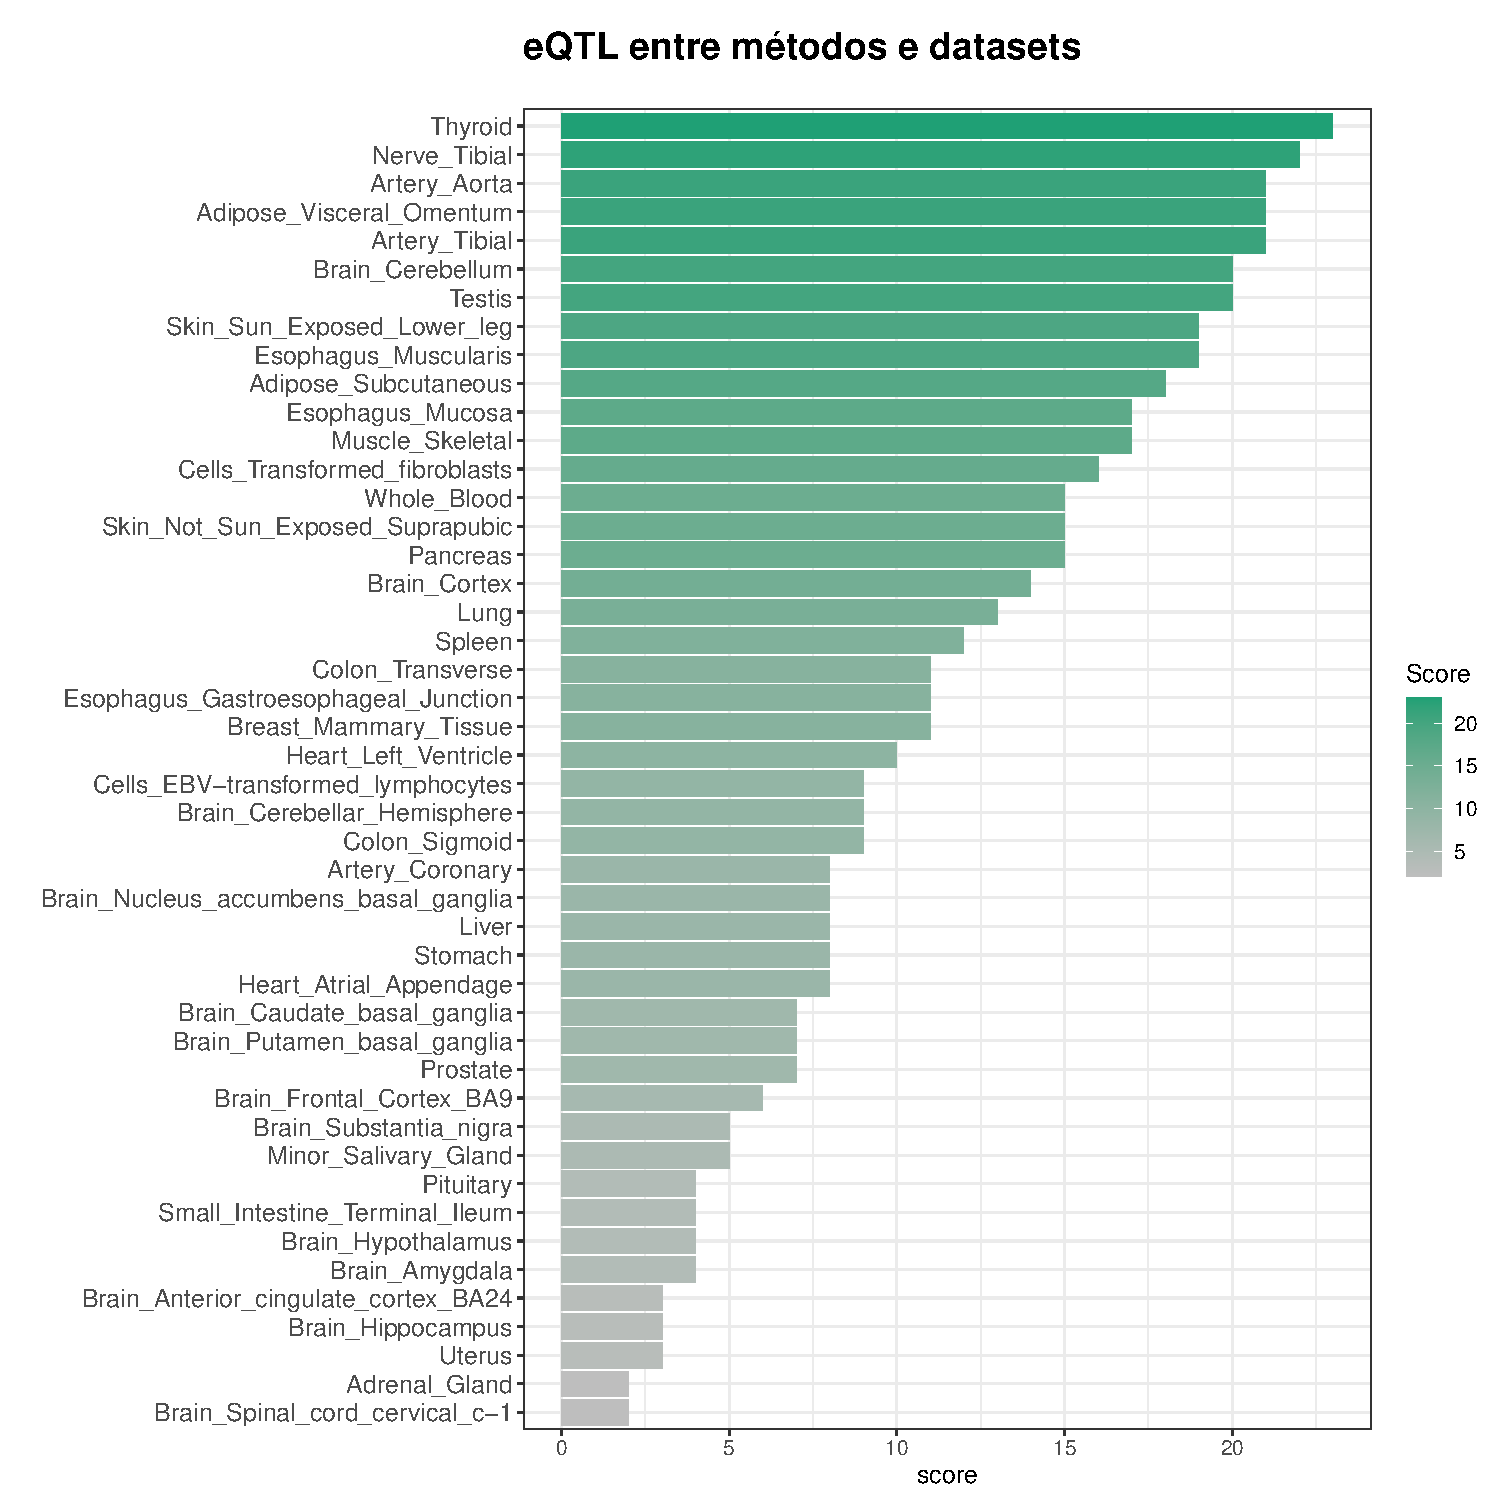
\includegraphics[width=1.0\linewidth]{overall_eqtl_score}
    \caption[Valores totais de eQTL para os alelos candidatos.]{Valores totais de eQTL para os alelos candidatos. Nesta abordagem, compilamos os resultados de eQTL para os métodos PBS e XP-EHH em ambos os datasets, e atribuímos um valor (\textsl{score}) para cada tecido somando o total de alelos candidatos que contribuem de forma significativa para a expressão de seu respectivo gene (positiva ou negativamente).}
    \label{fig:overall_eqtl_score}
\end{figure}

\begin{figure}[!htbp] % figura 2.14
    \centering
    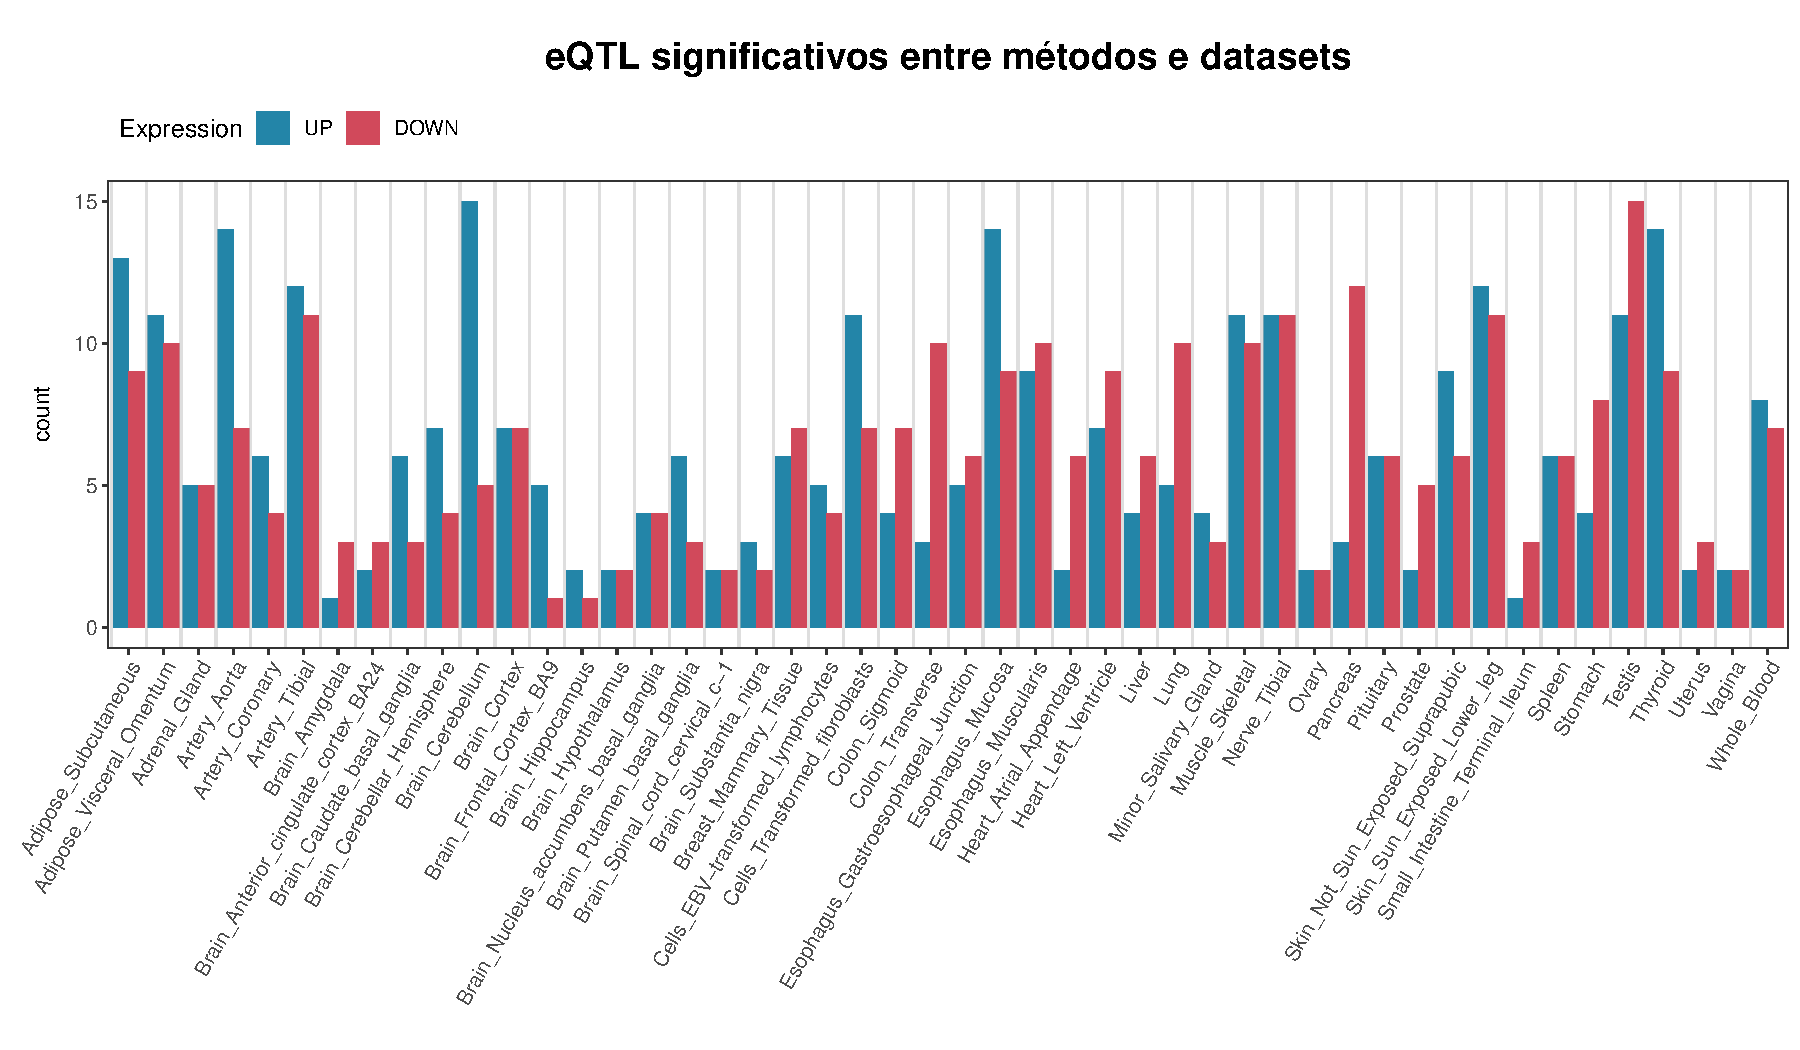
\includegraphics[width=1.0\linewidth]{overall_eqtl_count}
    \caption[Valores diferenciais de eQTL para os alelos candidatos.]{Valores diferenciais de eQTL para os alelos candidatos. Nesta abordagem, compilamos os resultados de eQTL para os métodos PBS e XP-EHH em ambos os datasets e somamos o total de alelos candidatos que contribuem de forma significativa para a expressão de seu respectivo gene, agrupando por categoria de expressão.}
    \label{fig:overall_eqtl_count}
\end{figure}

\FloatBarrier

\subsection{Enriquecimento Gênico}

Outra maneira de realizar o levantamento de fenótipos dado uma lista de genes são as análises de super-representação (ORA) e enriquecimento gênico (GSEA). Aplicamos estas análises nos bancos de dados públicos GWAS Catalog, KEGG e Gene Ontology. Primeiramente, utilizamos a plataforma Enrichr para análise ORA nos bancos GWAS Catalog e KEGG. Posteriormente, uma vez que esta plataforma não possibilita o uso de uma segunda lista de genes que sirvam de parâmetro (por padrão utiliza todos os genes humanos do banco de dados Ensembl), utilizamos duas outras ferramentas ─ FUMAGWAS e WebGestalt ─ que possibilitam o uso dessa lista para os bancos GWAS Catalog e KEGG, respectivamente. Adicionalmente, também rodamos a análise GSEA no banco de dados KEGG (WebGestalt).

Focando primeiramente no banco de dados do GWAS Catalog, no dataset S1, o método PBS resultou nos fenótipos “consumo de álcool”, “consumo de café” e “traços relacionados à obesidade” na abordagem por SNP quando considerado os SNPs do extremo 1\% da distribuição na plataforma Enrichr. Na plataforma FUMAGWAS, estes mesmos fenótipos foram detectados em conjunto com “consumo de café” e “traços relacionados à obesidade”. Este último também foi detectado no top 0,5\% da distribuição, em conjunto com “tolerância geral ao risco” (FDR < 0.038). No dataset S2, em ambas as plataformas, os termos “consumo de café” e “consumo de álcool”, de forma literal ou derivada, foram identificados em ambas as plataformas. Demais fenótipos identificados pelo método PBS no dataset S2 podem ser verificados na tabela \ref{tab:ds2_fumagwas_pbs_persnp}. Na abordagem por gene, o método PBS resultou nos mesmos fenótipos que na abordagem por SNP quando utilizada a plataforma Enrichr no dataset S1, enquanto o dataset S2 apresentou os mesmos termos em ambas as plataformas, mesmo quando selecionado o extremo 0,1\% dos genes (\autoref{tab:ds2_fumagwas_pbs_pergene}). Adicionalmente, quando consideramos o top 0,5\%, detectamos outros fenótipos como “mensuração de imunoglobulina”, “contagem de linfócitos”, “contagem de glóbulos brancos”, todos relacionados com o sistema imune, além de traços relacionados ao metabolismo energético (dados não mostrados).  

%tabela 2.12
\begin{table}[!htbp]
\centering

\begin{tabular}[t]{lrr}

\toprule
Fenótipo & -log$_{10}$(\emph{p}) & FDR\\
\midrule
Response to alcohol consumption (flushing response) & 8.9030 & 0.0000\\
Alcohol consumption (max-drinks) & 8.3391 & 0.0000\\
Systolic blood pressure x alcohol consumption interaction (2df test) & 7.2454 & 0.0000\\
Mean arterial pressure x alcohol consumption interaction (2df test) & 5.9580 & 0.0005\\
Alcohol dependence symptom count & 5.7618 & 0.0006\\
Diastolic blood pressure x alcohol consumption interaction (2df test) & 5.6333 & 0.0007\\
Coffee consumption & 5.0736 & 0.0022\\
Mean arterial pressure & 4.6972 & 0.0046\\
Alcohol consumption (drinkers vs non-drinkers) & 4.5856 & 0.0050\\
Aspartate aminotransferase levels & 4.5615 & 0.0050\\
Coronary heart disease & 3.9928 & 0.0168\\
Esophageal cancer & 3.7438 & 0.0273\\
\bottomrule

\end{tabular}

\caption{Fenótipos enriquecidos no banco GWASCatalog (FUMAGWAS), utilizando a abordagem por SNP no extremo 0,1\% da distribuição de PBS do dataset S2.}
\label{tab:ds2_fumagwas_pbs_persnp}

\end{table} % tabela 2.12

%tabela 2.13
\begin{table}[!htbp]
\centering

\begin{tabularx}{\linewidth}{Xrr}
\toprule
Fenótipo & -log$_{10}$(\emph{p}) & FDR\\
\midrule
Response to alcohol consumption (flushing response) & 10.3086 & 0.0000\\
Alcohol consumption (max-drinks) & 9.7437 & 0.0000\\
Alcohol dependence symptom count & 9.5183 & 0.0000\\
Mean arterial pressure x alcohol consumption interaction  & 7.3521 & 0.0000\\
Esophageal cancer & 7.0309 & 0.0000\\
Diastolic blood pressure x alcohol consumption interaction  & 7.0245 & 0.0000\\
Systolic blood pressure x alcohol consumption interaction  & 6.8588 & 0.0000\\
Coffee consumption & 6.4583 & 0.0001\\
Crohn's disease & 6.1587 & 0.0001\\
Diastolic blood pressure x alcohol consumption (light vs heavy)  & 6.0828 & 0.0001\\
Alcohol consumption (drinkers vs non-drinkers) & 5.2424 & 0.0009\\
Hypothyroidism & 5.1186 & 0.0012\\
Inflammatory bowel disease & 4.4465 & 0.0050\\
Serum uric acid levels & 4.3010 & 0.0065\\
Mean arterial pressure & 4.2357 & 0.0070\\
Alcohol consumption & 4.0574 & 0.0099\\
C-reactive protein levels or LDL-cholesterol levels (pleiotropy) & 3.9443 & 0.0121\\
Hematological and biochemical traits & 3.6485 & 0.0227\\
Aspartate aminotransferase levels & 3.4485 & 0.0340\\
Metabolic syndrome & 3.3372 & 0.0417\\
Body mass index & 3.2689 & 0.0465\\
\bottomrule
\end{tabularx}

\caption{Fenótipos enriquecidos no banco GWASCatalog (FUMAGWAS), utilizando a abordagem por gene no extremo 0,1\% da distribuição de PBS do dataset S2.}
\label{tab:ds2_fumagwas_pbs_pergene}

\end{table} % tabela 2.13

No método XP-EHH, o fenótipo sobressalente no dataset S1 foi “consumo de café”, em ambas as plataformas e nos três valores de corte de distribuição aplicados. Neste método, como no anterior, a plataforma FUMAGWAS apresentou mais termos significativamente enriquecidos quando comparado à plataforma Enrichr, mostrando uma importante influência da população gênica selecionada na análise. Ao considerar valores de corte mais liberais, como 0,5\% e 1\%, detectamos traços como “tecido adiposo subcutâneo”, “mortalidade por falha cardíaca”, “tolerância ao risco geral” e outros relacionados com o sistema imunológico, destacando-se doenças inflamatórias (\emph{e.g.} alergias, psoríase), além dos traços de consumo de café, álcool e cigarro. No dataset S2, os termos mais salientes foram termos relacionados a pressão sanguínea e contagem de leucótios, em conjunto com traços relacionaos ao consumo de café e álcool. De forma similar ao dataset S1, mais termos significativos foram identificados pela plataforma FUMAGWAS. Na análise por gene, identifica-se termos semelhantes ou idênticos àqueles identificados na abordagem por SNP.

\newpage

No método iHS, cinco termos enriquecidos apareceram quando considerado o extremo 0,1\% da distribuição pela plataforma FUMAGWAS, dataset S1 (\autoref{tab:ds1_fumagwas_ihs_persnp}) e, destes, três ─ “níveis de urato em indivíduos obesos”, “hipertrofia cardíaca” e “concentração de tiroxina livre” ─ apareceram também na plataforma Enrichr. Ao selecionar os valores  menos restritivos da distribuição, observa-se todos os termos identificados pelos métodos anteriores. Na abordagem por gene, apenas “consumo de café” está em convergência entre as plataformas, com demais termos possivelmente relacionados (\emph{e.g.} consumo de álcool e cigarro) presentes na plataforma Enrichr. No dataset S2, o termo “nascimento prematuro espontâneo moderado-tardio”, encontrado no dataset S1, foi detectado no extremo 0,5\% da distribuição, em conjunto com uma variedade de fatores. Para o método iHS, observa-se múltiplos termos significativos quando consideramos os top 0,5\% ou 1\% da distribuição por SNP. Dentre os fenótipos identificados, incluem-se diabetes tipo II, metabolismo, densidade mineral óssea, altura, pressão sistólica e diastólica, respota viral (\emph{e.g.} HIV, Epstein-Barr), contagem de leucócitos, e traços relacionados à picada de mosquito (também identificados no dataset S1).

%tabela 2.14
\begin{table}[!htbp]
\centering

\begin{tabular}[t]{lrr}
\toprule
Fenótipo & -log$_{10}$(\emph{p}) & FDR\\
\midrule
Urate levels in obese individuals & 4.6378 & 0.0245\\
Renal cell carcinoma & 4.5014 & 0.0245\\
Moderate-to-late spontaneous preterm birth & 4.3584 & 0.0245\\
Cardiac hypertrophy & 4.2299 & 0.0245\\
Free thyroxine concentration & 4.1703 & 0.0245\\
\bottomrule
\end{tabular}

\caption{Fenótipos enriquecidos no banco GWASCatalog (FUMAGWAS) no extremo 0,1\% da distribuição de iHS na abordagem por SNP, dataset S1.}
\label{tab:ds1_fumagwas_ihs_persnp}

\end{table}
 % tabela 2.14

\newpage

Na análise ORA realizada com o banco KEGG Pathway pelo WebGestalt, nenhuma via significativa apareceu em ambos os datasets, em nenhum dos métodos. A mesma análise realizada na plataforma Enrichr resultou apenas no termo “síntese e secreção de aldosterona” no dataset S1, quando considerado o top 1\% da distribuição de iHS na abordagem por SNP. No dataset S2, este mesmo termo apareceu no método PBS, também utilizando 1\% como valor de corte da distribuição (tabela \ref{tab:ds2_kegg_ora_persnp}). Dentre as vias de interesse identificadas nestas distribuições, destacam-se: vício à nicotina e morfina; sinapses glutamatérgicas e colinérgicas; arrastamento circadiano; sinalização adrenérgica em cardiomiócitos; síntese, secreção e ação do hormônio da paratireóide; síntese e secreção de cortisol e via de sinalização do estrogênio, discutidas no tópico \ref{sec:amazonia_discussion}. Adicionalmente, a abordagem por gene, pelo método XP-EHH, identificou três vias no dataset S2, sendo elas “via de sinalização IL-17”, que atua na mediação de respostas inflamatórias, “via de sinalização de receptores \textit{NOD-like}”, que atua em resposta à patógenos, e “lúpus eritematoso sistêmico”. A análise de GSEA, por sua vez, que considera todos os genes e seus respectivos valores, resultou em vias relacionadas ao metabolismo em ambos os datasets, nos métodos XP-EHH e iHS, respectivamente (\autoref{tab:gsea}).

%tabela 2.15
\begin{table}[!htbp]
\centering
\resizebox{\linewidth}{!}{
\begin{tabular}[h]{p{10cm}rrrrrr}

\toprule
\multirow[b]{3}{*}{Termo} & \multicolumn{6}{c}{iHS} \\
\cmidrule(l{3pt}r{3pt}){2-7}
\multicolumn{1}{c}{ } & \multicolumn{3}{c}{Top 0,5\%} & \multicolumn{3}{c}{Top 1\%} \\
\cmidrule(l{3pt}r{3pt}){2-4} \cmidrule(l{3pt}r{3pt}){5-7}
 & Score & $-log_{10}(p)$ & FDR & Score & $-log_{10}(p)$ & FDR\\
%Termo & Score & -log$_{10}$(\emph{p}) & FDR & Score & -log$_{10}$(\emph{p}) & FDR\\
\midrule

\cellcolor{gray!6}{Nicotine addiction} & \cellcolor{gray!6}{59.9289} & \cellcolor{gray!6}{3.77} & \cellcolor{gray!6}{0.0224} & \cellcolor{gray!6}{27.3208} & \cellcolor{gray!6}{2.8188} & \cellcolor{gray!6}{0.0151}\\
Circadian entrainment & 36.5269 & 3.7954 & 0.0224 & 54.9613 & 5.7767 & 1e-04\\
\cellcolor{gray!6}{Arrhythmogenic right ventricular cardiomyopathy (ARVC)} & \cellcolor{gray!6}{37.7809} & \cellcolor{gray!6}{3.5226} & \cellcolor{gray!6}{0.0264} & \cellcolor{gray!6}{93.5812} & \cellcolor{gray!6}{7.185} & \cellcolor{gray!6}{0}\\
Glutamatergic synapse & 25.5608 & 3.1838 & 0.0346 & 60.5433 & 6.4693 & 0\\
\cellcolor{gray!6}{Cholinergic synapse} & \cellcolor{gray!6}{26.6032} & \cellcolor{gray!6}{3.249} & \cellcolor{gray!6}{0.0346} & \cellcolor{gray!6}{73.4442} & \cellcolor{gray!6}{7.2541} & \cellcolor{gray!6}{0}\\
Oxytocin signaling pathway & - & - & - & 58.3875 & 6.9434 & 0\\
\cellcolor{gray!6}{Adrenergic signaling in cardiomyocytes} & \cellcolor{gray!6}{-} & \cellcolor{gray!6}{-} & \cellcolor{gray!6}{-} & \cellcolor{gray!6}{51.2635} & \cellcolor{gray!6}{6.2798} & \cellcolor{gray!6}{0}\\
Morphine addiction & - & - & - & 53.6082 & 5.5698 & 1e-04\\
\cellcolor{gray!6}{GABAergic synapse} & \cellcolor{gray!6}{-} & \cellcolor{gray!6}{-} & \cellcolor{gray!6}{-} & \cellcolor{gray!6}{46.7865} & \cellcolor{gray!6}{5.0808} & \cellcolor{gray!6}{3e-04}\\
Dilated cardiomyopathy (DCM) & - & - & - & 44.3123 & 4.9463 & 4e-04\\
\cellcolor{gray!6}{Parathyroid hormone synthesis, secretion and action} & \cellcolor{gray!6}{-} & \cellcolor{gray!6}{-} & \cellcolor{gray!6}{-} & \cellcolor{gray!6}{36.7548} & \cellcolor{gray!6}{4.6071} & \cellcolor{gray!6}{7e-04}\\
Aldosterone synthesis and secretion & - & - & - & 36.8837 & 4.5082 & 8e-04\\
\cellcolor{gray!6}{Calcium signaling pathway} & \cellcolor{gray!6}{-} & \cellcolor{gray!6}{-} & \cellcolor{gray!6}{-} & \cellcolor{gray!6}{25.4194} & \cellcolor{gray!6}{4.2394} & \cellcolor{gray!6}{0.0014}\\
Hypertrophic cardiomyopathy (HCM) & - & - & - & 34.5165 & 4.1371 & 0.0016\\
\cellcolor{gray!6}{Long-term depression} & \cellcolor{gray!6}{-} & \cellcolor{gray!6}{-} & \cellcolor{gray!6}{-} & \cellcolor{gray!6}{38.4978} & \cellcolor{gray!6}{3.9611} & \cellcolor{gray!6}{0.0023}\\
Relaxin signaling pathway & - & - & - & 26.0753 & 3.907 & 0.0024\\
\cellcolor{gray!6}{cAMP signaling pathway} & \cellcolor{gray!6}{-} & \cellcolor{gray!6}{-} & \cellcolor{gray!6}{-} & \cellcolor{gray!6}{20.7287} & \cellcolor{gray!6}{3.7944} & \cellcolor{gray!6}{0.0029}\\
Cortisol synthesis and secretion & - & - & - & 31.8089 & 3.6148 & 0.004\\
\cellcolor{gray!6}{Estrogen signaling pathway} & \cellcolor{gray!6}{-} & \cellcolor{gray!6}{-} & \cellcolor{gray!6}{-} & \cellcolor{gray!6}{22.6164} & \cellcolor{gray!6}{3.6038} & \cellcolor{gray!6}{0.004}\\
Insulin secretion & - & - & - & 26.6092 & 3.5183 & 0.0046\\
\cellcolor{gray!6}{Serotonergic synapse} & \cellcolor{gray!6}{-} & \cellcolor{gray!6}{-} & \cellcolor{gray!6}{-} & \cellcolor{gray!6}{20.72} & \cellcolor{gray!6}{3.228} & \cellcolor{gray!6}{0.0086}\\
Taste transduction & - & - & - & 22.6849 & 3.1429 & 0.01\\
\cellcolor{gray!6}{Gap junction} & \cellcolor{gray!6}{-} & \cellcolor{gray!6}{-} & \cellcolor{gray!6}{-} & \cellcolor{gray!6}{19.5286} & \cellcolor{gray!6}{2.8997} & \cellcolor{gray!6}{0.0141}\\
Long-term potentiation & - & - & - & 22.2306 & 2.915 & 0.0141\\
\cellcolor{gray!6}{Vascular smooth muscle contraction} & \cellcolor{gray!6}{-} & \cellcolor{gray!6}{-} & \cellcolor{gray!6}{-} & \cellcolor{gray!6}{16.7855} & \cellcolor{gray!6}{2.9181} & \cellcolor{gray!6}{0.0141}\\
Cushing syndrome & - & - & - & 15.9446 & 2.931 & 0.0141\\
\cellcolor{gray!6}{Dopaminergic synapse} & \cellcolor{gray!6}{-} & \cellcolor{gray!6}{-} & \cellcolor{gray!6}{-} & \cellcolor{gray!6}{17.1484} & \cellcolor{gray!6}{2.9551} & \cellcolor{gray!6}{0.0141}\\
Rap1 signaling pathway & - & - & - & 14.0141 & 2.8604 & 0.0148\\
\cellcolor{gray!6}{Inflammatory mediator regulation of TRP channels} & \cellcolor{gray!6}{-} & \cellcolor{gray!6}{-} & \cellcolor{gray!6}{-} & \cellcolor{gray!6}{18.0156} & \cellcolor{gray!6}{2.8474} & \cellcolor{gray!6}{0.0148}\\
Salivary secretion & - & - & - & 18.4205 & 2.8084 & 0.0151\\
\cellcolor{gray!6}{Retrograde endocannabinoid signaling} & \cellcolor{gray!6}{-} & \cellcolor{gray!6}{-} & \cellcolor{gray!6}{-} & \cellcolor{gray!6}{14.9165} & \cellcolor{gray!6}{2.7683} & \cellcolor{gray!6}{0.016}\\
GnRH signaling pathway & - & - & - & 16.8997 & 2.6773 & 0.0191\\
\cellcolor{gray!6}{Thyroid hormone synthesis} & \cellcolor{gray!6}{-} & \cellcolor{gray!6}{-} & \cellcolor{gray!6}{-} & \cellcolor{gray!6}{17.3365} & \cellcolor{gray!6}{2.5584} & \cellcolor{gray!6}{0.0244}\\
Gastric acid secretion & - & - & - & 16.7532 & 2.5117 & 0.0263\\
\cellcolor{gray!6}{Cell adhesion molecules (CAMs)} & \cellcolor{gray!6}{-} & \cellcolor{gray!6}{-} & \cellcolor{gray!6}{-} & \cellcolor{gray!6}{12.7955} & \cellcolor{gray!6}{2.4777} & \cellcolor{gray!6}{0.0272}\\
Pancreatic secretion & - & - & - & 14.6909 & 2.4735 & 0.0272\\
\cellcolor{gray!6}{HIF-1 signaling pathway} & \cellcolor{gray!6}{-} & \cellcolor{gray!6}{-} & \cellcolor{gray!6}{-} & \cellcolor{gray!6}{13.906} & \cellcolor{gray!6}{2.3967} & \cellcolor{gray!6}{0.0315}\\
Apelin signaling pathway & - & - & - & 12.0653 & 2.3478 & 0.0344\\
\cellcolor{gray!6}{cGMP-PKG signaling pathway} & \cellcolor{gray!6}{-} & \cellcolor{gray!6}{-} & \cellcolor{gray!6}{-} & \cellcolor{gray!6}{10.5422} & \cellcolor{gray!6}{2.2295} & \cellcolor{gray!6}{0.044}\\
Axon guidance & - & - & - & 9.9084 & 2.1727 & 0.0489\\

\bottomrule
\end{tabular}}

\caption{ORA utilizando o banco de dados KEGG - Dataset S2.}
\label{tab:ds2_kegg_ora_persnp}

\end{table}
 % tabela 2.15

%tabela 2.16
\begin{table}[!htbp]
\centering

\begin{tabularx}{.9\textwidth}{Xlrr}

\toprule
Via de Sinalização & Enriquecimento & \emph{p}-valor & FDR\\
\midrule
Ascorbate and aldarate metabolism & 2.3517 & 0.0000 & 0.0000\\
Pentose and glucuronate interconversions & 2.0084 & 0.0021 & 0.0087\\
Porphyrin and chlorophyll metabolism & 1.9648 & 0.0000 & 0.0102\\
Retinol metabolism & 1.8890 & 0.0000 & 0.0195\\
Vitamin B6 metabolism & 1.7817 & 0.0020 & 0.0386\\
Steroid hormone biosynthesis & 1.7879 & 0.0022 & 0.0444\\

\bottomrule
\end{tabularx}

\caption{GSEA utilizando o banco de dados KEGG e resultados de XP-EHH no dataset S2.}
\label{tab:gsea}

\end{table}
 % tabela 2.16

Por fim, utilizamos o banco de dados da Gene Ontology, focando exclusivamente nos termos pertencentes a processos biológicos. Realizamos uma análise ampla abrangendo todos os termos disponíveis, bem como reduzindo a quantidade de termos a fim de reduzir redundância de processos similares (utilizando termos GO slim, vide material e métodos). Adicionalmente, dado a alta virulência dos ambientes de floresta tropicais, verificamos especificamente os termos GO pertencentes ao sistema imunológico (GO:0002376).

Nas análises utilizando todos os termos GO, na abordagem por SNP, poucos ou nenhum termos surgiram no dataset S1 quando utilizando os extremos 0,1\% e 0,5\% dos três métodos aplicados. Contudo, utilizando os top 1\% da distribuição, encontramos termos relacionados ao crescimento no método XP-EHH e múltiplos termos para o método iHS, incluindo vias cardiovasculares (\autoref{tab:ds1_go_all_persnp}). No dataset S2, o extremo 0,5\% das distribuições de iHS e XP-EHH já possibilitou identificar termos significativos, sobressaindo termos relacionados ao sistema imunológico pelo método XP-EHH (\autoref{tab:ds2_go_all_pergene}). Na abordagem por gene, os termos “regeneração do tecido muscular esquelético” e “metilação ou desmetilação de DNA” foram identificados no dataset S1 (método PBS), e apenas o método XP-EHH retornou termos significativos no dataset S2, sobressaindo termos do sistema imune (\autoref{tab:ds2_go_all_pergene}). Na análise de termos GO não-redundantes, na abordagem por SNP, em ambos os datasets aparecerem os termos “crescimento”, “locomoção” e “processo do sistema nervoso”, enquanto que no dataset S2 apareceu também, dentre termos relacionados a processos celulares, o termo “processo do sistema circulatório”. Adicionalmente, na abordagem por gene apareceu “desenvolvimento embrionário” no dataset S1, e os termos “metabolismo de carboidratos” e “resposta ao estresse” no dataset S2.

%tabela 2.17
\begin{table}[!htbp]
\centering

\begin{tabular}[!htb]{m{2cm}m{9cm}rr}

\toprule
Método & Termo & -log$_{10}$(\emph{p}) & FDR\\

\rowcolor{gray!6}
\midrule
 & developmental growth & 6.002302 & 0.002\\
\rowcolor{gray!6}
 & growth & 5.923484 & 0.002\\
\rowcolor{gray!6}
 & multicellular organismal process & 4.799597 & 0.040\\
\rowcolor{gray!6}

\multirow{-4}{*}{\raggedright\arraybackslash XP-EHH} & regulation of localization & 4.758747 & 0.040\\
\cmidrule[0.5pt]{1-4}
 & regulation of blood circulation & 6.291592 & 0.000\\
 & cardiac conduction & 5.964111 & 0.000\\
 & inorganic cation transmembrane transport & 5.887296 & 0.000\\
 & regulation of heart contraction & 5.851375 & 0.000\\
 & cation transmembrane transport & 5.796583 & 0.000\\
 & regulation of system process & 5.696401 & 0.000\\
 & modulation of chemical synaptic transmission & 5.616438 & 0.002\\
 & regulation of trans-synaptic signaling & 5.592960 & 0.002\\
 & sensory perception & 5.474760 & 0.008\\
 & regulation of biological quality & 5.431910 & 0.010\\
 & regulation of localization & 5.336457 & 0.012\\
 & multicellular organismal signaling & 5.272507 & 0.018\\
 & system process & 5.222667 & 0.018\\
 & ion transmembrane transport & 5.203898 & 0.018\\
 & inorganic ion transmembrane transport & 5.032140 & 0.020\\
 & cation transport & 4.976156 & 0.026\\

\multirow{-17}{*}{\raggedright\arraybackslash iHS} & multicellular organismal process & 4.936052 & 0.028\\
\bottomrule
\end{tabular}

\caption{Termos enriquecidos do banco Gene Ontology no dataset S1, abordagem por SNP.}
\label{tab:ds1_go_all_persnp}

\end{table}
 % tabela 2.17

%tabela 2.18
\begin{table}[!htbp]
\centering

\begin{tabular}[!htbp]{llrr}
\toprule
Método & Termo & -log10(p) & FDR\\
\rowcolor{gray!6}
\midrule
 & cellular response to interferon-gamma & 6.802781 & 0.000\\
\rowcolor{gray!6}
 & response to interferon-gamma & 6.116870 & 0.004\\
\rowcolor{gray!6}
 & defense response to protozoan & 5.332370 & 0.012\\
\rowcolor{gray!6}

\multirow{-4}{*}{\raggedright\arraybackslash \makecell[l]{XP-EHH \\(top 0,5\%)}} & response to protozoan & 5.332370 & 0.012\\
\cmidrule{1-4}
 & protein-DNA complex assembly & 6.110807 & 0.002\\
 & cytokine-mediated signaling pathway & 5.758698 & 0.004\\
 & regulation of multicellular organismal process & 5.705118 & 0.004\\
 & protein-DNA complex subunit organization & 5.286646 & 0.016\\
 & DNA replication-dependent nucleosome assembly & 5.073446 & 0.026\\
 & DNA replication-dependent nucleosome organization & 5.073446 & 0.026\\
 & rDNA heterochromatin assembly & 5.000396 & 0.028\\
 & nucleosome assembly & 4.970933 & 0.030\\
 & regulation of immune system process & 4.850650 & 0.038\\

\multirow{-10}{*}{\raggedright\arraybackslash \makecell[l]{XP-EHH \\(top 1\%)}} & cellular response to interferon-gamma & 4.792833 & 0.038\\
\bottomrule
\end{tabular}

\caption{Termos enriquecidos do banco Gene Ontology no dataset S2, abordagem por gene.}
\label{tab:ds2_go_all_pergene}

\end{table}
 % tabela 2.19

Ao analisar especificamente termos GO do sistema imune, exceto pela “ativação da célula T envolvida na resposta imune” pelo método iHS na abordagem por SNP (\emph{p}-valor = 0,000131; FDR = 0,04), nenhum outro termo foi detectado como significativo após correção dos \emph{p}-valores. Contudo, no dataset S2, múltiplos termos aparecem para os métodos PBS e XP-EHH na abordagem por SNP (\autoref{tab:ds2_go_immune_persnp}), bem como no método XP-EHH na abordagem por gene \ref{tab:ds2_go_immune_pergene}) (mesmos termos identificados na abordagem por SNP).

%tabela 2.19
\begin{table}[H]
\centering

\begin{tabular}[!htbp]{llrr}
\toprule
Método & Term & -log$_{10}$(\emph{p}) & FDR\\
\rowcolor{gray!6}
\midrule
 & positive thymic T cell selection & 4.802562 & 0.022\\
\rowcolor{gray!6}

 & negative thymic T cell selection & 4.802562 & 0.022\\
\rowcolor{gray!6}

\multirow{-3}{*}{\raggedright\arraybackslash PBS} & negative T cell selection & 4.679098 & 0.034\\
\cmidrule{1-4}
 & response to biotic stimulus & 5.748423 & 0.006\\

 & response to external biotic stimulus & 5.477667 & 0.012\\

 & negative regulation of cell communication & 5.368043 & 0.014\\

\multirow{-4}{*}{\raggedright\arraybackslash XP-EHH} & negative regulation of signaling & 5.356821 & 0.016\\
\bottomrule
\end{tabular}

\caption{Termos enriquecidos do banco Gene Ontology no dataset S2, abordagem por SNP.}
\label{tab:ds2_go_immune_persnp}

\end{table}
 % tabela 2.18

%tabela 2.20
\begin{table}[!htb]
\centering

\begin{tabularx}{.75\linewidth}{Xrr}

\toprule
Termo & -log$_{10}$(\emph{p}) & FDR\\
\midrule
\addlinespace[0.3em]
\multicolumn{3}{l}{\textbf{PBS}}\\
\midrule[0.5pt]
positive thymic T cell selection & 2.817464 & 0.050\\
negative thymic T cell selection & 2.817464 & 0.050\\
\addlinespace[0.3em]
\midrule[0.5pt]
\multicolumn{3}{l}{\textbf{XP-EHH}}\\
\midrule[0.5pt]
granulocyte migration & 4.661809 & 0.000\\
granulocyte chemotaxis & 4.077900 & 0.006\\
myeloid leukocyte migration & 3.924738 & 0.010\\
neutrophil migration & 3.864530 & 0.012\\
leukocyte chemotaxis & 3.722748 & 0.012\\
neutrophil chemotaxis & 3.193541 & 0.040\\
\bottomrule
\end{tabularx}

\caption{Termos GO do sistema imune identificados na abordagem por gene, dataset S2.}
\label{tab:ds2_go_immune_pergene}

\end{table}
 % tabela 2.20

\hspace{2em}

Em conjunto, as análises de enriquecimento gênico revelaram fenótipos relacionados ao desenvolvimento corporal (\emph{e.g.} crescimento, massa corporal, obesidade, nascimento prematuro), vias cardíacas (e.g. pressão sistólica, diastólica e arterial, hipertrofia cardíaca, doença coronariana, sinalização adrenérgica em cardiomiócitos), a diabetes (\emph{e.g.} diabetes tipo II, traços glicêmicos e secreção de insulina), à tireoide (\emph{e.g.} síntese do hormônio tireoidiano, diferenciação das células Th1 e Th2, hipotireoidismo, concentração de tiroxina livre), ao metabolismo, sistema imunológico, sobretudo na quantidade, resposta e diferenciação de leucócitos (especialmente linfócito T), bem como comportamentos de vício, como alcoolismo e consumo de café.

%\clearpage
\subsection{Convergência Evolutiva (Metanálise)}

A fim de comparar nossos resultados com aqueles já publicados na literatura sobre seleção em populações nativas de Floresta Tropical, comparamos os resultados de 13 artigos de nosso conhecimento com os nossos resultados. A tabela \ref{tab:metanalysis} sumariza as populações e métodos utilizados para detecção de seleção positiva nos artigos avaliados.

\vspace{\onelineskip}

%tabela 2.21
\begin{table}[!htbp]

\small
\centering
\renewcommand{\arraystretch}{1.4}
\renewcommand\tabularxcolumn[1]{m{#1}}

\begin{tabularx}{\textwidth}{lXl}

\toprule
Autores & Populações & Métodos de seleção\\
\midrule
\cellcolor{gray!6}{Amorim et al. (2015)} & \cellcolor{gray!6}{Biaka, Mbuti, Surui, Karitiana} & \cellcolor{gray!6}{BayeScan}\\
Bergey et al. (2018) & Batwa, Andamanese & PBS, PBSi, Bayenv\\
\cellcolor{gray!6}{Harrison et al. (2019)} & \cellcolor{gray!6}{Batwa} & \cellcolor{gray!6}{PBS, iHS}\\
Hsieh et al. (2016) & Biaka, Baka & iHS, G2D\\
\cellcolor{gray!6}{Jarvis et al. (2012)} & \cellcolor{gray!6}{Bakola, Baka, Bedzan} & \cellcolor{gray!6}{LSBL, XP-EHH, iHS}\\
Lachance et al. (2012) & Western Pygmy,l Hadza, Sandawe & LSBL, AIMs\\
\cellcolor{gray!6}{López Herráez et al. (2009)} & \cellcolor{gray!6}{Pygmy, Surui, Karitiana} & \cellcolor{gray!6}{lnRsb}\\
Miligliano et al. (2013) & Biaka, Mbuti, Aeta, Batak, Agta + 2 & XP-EHH, iHS\\
\cellcolor{gray!6}{Perry et al. (2014)} & \cellcolor{gray!6}{Baka, Batwa} & \cellcolor{gray!6}{Fst, iHS, BayeScan}\\
Scheinfeldt et al. (2019) & Hadza, Sandawe, Dahalo, Sabue + 6 outras & D, iHS, XP-CLR\\
\bottomrule

\end{tabularx}

\caption{Estudos avaliados na metanálise para convergência evolutiva.}
\label{tab:metanalysis}

\vspace{2em}

\end{table}
 % tabela 2.21

Para cada artigo, consideramos a intersecção dos genes candidatos que constam nos artigos com a união dos genes candidatos levantados na presente pesquisa, pelos três métodos de seleção (\emph{i.e.} PBS, XP-EHH e iHS), em ambos os datasets. De forma similar ao item \ref{subsec:amazonia_results_annotfuncional}, realizamos a anotação funcional dos genes de intersecção, utilizando tanto os bancos Ensembl como GWAS Catalog. A \autoref{tab:metanalysis_ensembl} apresenta os resultados dos trinta primeiros fenótipos com mais genes candidatos, levantados pelo banco de dados Ensembl, com interseção entre os métodos e estudos avaliados. As colunas “Genes” e “Estudos” denotam quantos únicos genes e estudos foram mapeados para um dado fenótipo, respectivamente, enquanto as demais colunas denotam quantos genes mapeados para o respectivo fenótipo apareceram entre os métodos e datasets, podendo (e com provável) repetição de gene-fenótipo entre métodos e datasets (\emph{e.g.} um fenótipo cujo gene apareceu em mais de um método). Para evitar redundância de resultados, não incluímos os resultados do banco GWAS Catalog, visto que os resultados foram similares (dados não mostrados).

%tabela 2.22
\begin{table}[!ht]
\centering

\renewcommand{\arraystretch}{1.2}

\resizebox{\linewidth}{!}{
\begin{tabular}[!ht]{lrrrrrrrr}

\toprule
\multicolumn{3}{c}{ } & \multicolumn{3}{c}{Dataset S1} & \multicolumn{3}{c}{Dataset S2} \\
\cmidrule(l{3pt}r{3pt}){4-6} \cmidrule(l{3pt}r{3pt}){7-9}
Fenótipo & Genes & Estudos & PBS & XP-EHH & iHS & PBS & XP-EHH & iHS\\
\midrule

\cellcolor{gray!6}{Body Mass Index} & \cellcolor{gray!6}{35} & \cellcolor{gray!6}{7} & \cellcolor{gray!6}{5} & \cellcolor{gray!6}{4} & \cellcolor{gray!6}{11} & \cellcolor{gray!6}{4} & \cellcolor{gray!6}{2} & \cellcolor{gray!6}{15}\\
Blood pressure & 30 & 9 & 4 & 3 & 8 & 1 & 3 & 16\\
\cellcolor{gray!6}{Cholesterol, HDL} & \cellcolor{gray!6}{24} & \cellcolor{gray!6}{7} & \cellcolor{gray!6}{3} & \cellcolor{gray!6}{2} & \cellcolor{gray!6}{7} & \cellcolor{gray!6}{4} & \cellcolor{gray!6}{0} & \cellcolor{gray!6}{14}\\
Metabolite levels & 23 & 8 & 5 & 3 & 6 & 2 & 1 & 12\\
\cellcolor{gray!6}{Body Height} & \cellcolor{gray!6}{22} & \cellcolor{gray!6}{7} & \cellcolor{gray!6}{3} & \cellcolor{gray!6}{3} & \cellcolor{gray!6}{5} & \cellcolor{gray!6}{1} & \cellcolor{gray!6}{3} & \cellcolor{gray!6}{9}\\
Blood protein levels & 21 & 8 & 2 & 4 & 5 & 1 & 1 & 7\\
\cellcolor{gray!6}{Height} & \cellcolor{gray!6}{21} & \cellcolor{gray!6}{8} & \cellcolor{gray!6}{2} & \cellcolor{gray!6}{1} & \cellcolor{gray!6}{4} & \cellcolor{gray!6}{1} & \cellcolor{gray!6}{1} & \cellcolor{gray!6}{16}\\
Triglycerides & 20 & 8 & 1 & 1 & 2 & 0 & 1 & 14\\
\cellcolor{gray!6}{Asthma} & \cellcolor{gray!6}{19} & \cellcolor{gray!6}{7} & \cellcolor{gray!6}{1} & \cellcolor{gray!6}{1} & \cellcolor{gray!6}{4} & \cellcolor{gray!6}{2} & \cellcolor{gray!6}{4} & \cellcolor{gray!6}{8}\\
Cholesterol, LDL & 19 & 7 & 1 & 2 & 9 & 1 & 2 & 10\\
\cellcolor{gray!6}{Refractive error} & \cellcolor{gray!6}{19} & \cellcolor{gray!6}{7} & \cellcolor{gray!6}{2} & \cellcolor{gray!6}{4} & \cellcolor{gray!6}{5} & \cellcolor{gray!6}{1} & \cellcolor{gray!6}{0} & \cellcolor{gray!6}{12}\\
Myocardial infarction & 18 & 7 & 3 & 2 & 5 & 1 & 1 & 7\\
\cellcolor{gray!6}{Autism spectrum disorder or schizophrenia} & \cellcolor{gray!6}{17} & \cellcolor{gray!6}{6} & \cellcolor{gray!6}{1} & \cellcolor{gray!6}{5} & \cellcolor{gray!6}{2} & \cellcolor{gray!6}{1} & \cellcolor{gray!6}{2} & \cellcolor{gray!6}{8}\\
Body Weight & 17 & 7 & 1 & 2 & 7 & 2 & 0 & 9\\
\cellcolor{gray!6}{Cholesterol} & \cellcolor{gray!6}{17} & \cellcolor{gray!6}{7} & \cellcolor{gray!6}{1} & \cellcolor{gray!6}{3} & \cellcolor{gray!6}{5} & \cellcolor{gray!6}{0} & \cellcolor{gray!6}{2} & \cellcolor{gray!6}{11}\\
Echocardiography & 17 & 8 & 2 & 0 & 7 & 2 & 0 & 9\\
\cellcolor{gray!6}{Stroke} & \cellcolor{gray!6}{17} & \cellcolor{gray!6}{8} & \cellcolor{gray!6}{1} & \cellcolor{gray!6}{2} & \cellcolor{gray!6}{3} & \cellcolor{gray!6}{0} & \cellcolor{gray!6}{3} & \cellcolor{gray!6}{13}\\
Heart Rate & 16 & 6 & 2 & 3 & 3 & 0 & 1 & 9\\
\cellcolor{gray!6}{Iron} & \cellcolor{gray!6}{16} & \cellcolor{gray!6}{7} & \cellcolor{gray!6}{1} & \cellcolor{gray!6}{2} & \cellcolor{gray!6}{0} & \cellcolor{gray!6}{0} & \cellcolor{gray!6}{2} & \cellcolor{gray!6}{13}\\
Heel bone mineral density & 15 & 6 & 2 & 3 & 2 & 2 & 0 & 7\\
\cellcolor{gray!6}{Obesity-related traits} & \cellcolor{gray!6}{15} & \cellcolor{gray!6}{7} & \cellcolor{gray!6}{2} & \cellcolor{gray!6}{1} & \cellcolor{gray!6}{3} & \cellcolor{gray!6}{0} & \cellcolor{gray!6}{2} & \cellcolor{gray!6}{11}\\
Pulse pressure & 14 & 6 & 1 & 1 & 3 & 0 & 0 & 10\\
\cellcolor{gray!6}{Chronotype} & \cellcolor{gray!6}{13} & \cellcolor{gray!6}{6} & \cellcolor{gray!6}{1} & \cellcolor{gray!6}{0} & \cellcolor{gray!6}{3} & \cellcolor{gray!6}{1} & \cellcolor{gray!6}{0} & \cellcolor{gray!6}{9}\\
Erythrocyte Count & 13 & 6 & 3 & 3 & 8 & 1 & 0 & 4\\
\cellcolor{gray!6}{Crohn's disease} & \cellcolor{gray!6}{12} & \cellcolor{gray!6}{7} & \cellcolor{gray!6}{0} & \cellcolor{gray!6}{3} & \cellcolor{gray!6}{4} & \cellcolor{gray!6}{0} & \cellcolor{gray!6}{4} & \cellcolor{gray!6}{4}\\
Estimated glomerular filtration rate & 12 & 6 & 1 & 2 & 0 & 3 & 1 & 4\\
\cellcolor{gray!6}{Respiratory Function Tests} & \cellcolor{gray!6}{12} & \cellcolor{gray!6}{7} & \cellcolor{gray!6}{1} & \cellcolor{gray!6}{2} & \cellcolor{gray!6}{5} & \cellcolor{gray!6}{1} & \cellcolor{gray!6}{0} & \cellcolor{gray!6}{9}\\
Coronary Artery Disease & 11 & 6 & 0 & 3 & 3 & 1 & 0 & 7\\
\cellcolor{gray!6}{Hemoglobin S} & \cellcolor{gray!6}{11} & \cellcolor{gray!6}{5} & \cellcolor{gray!6}{1} & \cellcolor{gray!6}{2} & \cellcolor{gray!6}{4} & \cellcolor{gray!6}{1} & \cellcolor{gray!6}{1} & \cellcolor{gray!6}{5}\\
Lipids & 11 & 6 & 1 & 2 & 4 & 1 & 0 & 6\\
\bottomrule

\end{tabular}}

\caption{Fenótipos mapeados aos genes candidatos com sinais de convergência evolutiva em populações caçadoras-coletoras de florestas tropicais (banco de dados Ensembl).}
\label{tab:metanalysis_ensembl}

\end{table}
 % tabela 2.22

\clearpage
\subsection{Estrutura de Arquivos no Repositório Mendeley}

Devido à estrutura metodológica deste trabalho, utilizando dois conjunto de dados, três testes de neutralidade (PBS, XP-EHH, iHS), duas abordagens (por SNP e por gene), quatro plataformas de enriquecimento gênico (Enrichr, FUMAGWAS, WebGestalt, GOATOOLS), análise em três banco de dados públicos (GWASCatalog, KEGG e GO), sendo este último banco dividido em termos não redundantes ou exclusivos do sistema imune, bem como anotação funcional e metanálise, uma variedade de gráficos e tabelas resultaram destas análises, tanto separadamente quanto em conjunto (intersecção dos resultados). Ainda, nas análises de enriquecimento gênico, aplicamos diferentes valores de corte para identificar genes candidatos (e.g. top 0,5\% e 1\%), uma vez que, utilizando o padrão nas análises de varredura genômica (\emph{i.e.} top 0,1\%), não encontramos termos significativos dada a quantidade insuficiente de genes para este tipo de análise. Assim, exceto as análises de estrutura populacional, todos os gráficos e tabelas das demais análises foram depositadas no banco de dados da Mendeley (\url{http://dx.doi.org/10.17632/gztff7wmjt.1}) com dois objetivos principais: 1) fornecer figuras em alta resolução nos formatos .png e .pdf e 2) promover a transparência da pesquisa científica.

As figuras e tabelas estão alocadas nas pastas figures e tables, respectivamente. A convenção de nomenclatura dos arquivos é \textsl{dataset} (ds1 ou ds2) + \textsl{método} + \textsl{modo}+ \textsl{descrição} (\emph{e.g.} ds1\_pbsw\_persnp.pdf). O modo corresponde à abordagem (por SNP ou por gene). Caso não tenha informação sobre o dataset no início, pode-se supor que se trata dos dois em conjunto. A descrição pode ou não estar presente. Por fim, para verificar qual script gerou uma figura/tabela, pode-se procurar pelo nome da figura/table (sem extensão) no arquivo \href{https://github.com/cmcouto-silva/tese/blob/main/Snakefile}{Snakefile} do repositório da tese.


%% ------------------------------------------------------------------------- %%
%% ------------------------------ DISCUSSÃO -------------------------------- %%
%% ------------------------------------------------------------------------- %%

%\cleardoublepage

\clearpage
\section{DISCUSSÃO}
\label{sec:amazonia_discussion}

\subsection{Varreduras Adaptativas e Enriquecimento Gênico}

Em conjunto, os resultados das varreduras adaptativas e de enriquecimento gênico identificaram vias relacionadas à estrutura corporal, sistema cardiovascular, sistema imune, comportamentos de risco, bem como metabolismo, sobressaindo-se fenótipos ligados à diabetes e tireoide. Cada um destes fenótipos será discutido separadamente a seguir, após uma breve análise da distribuição dos resultados.

Pode-se observar que, nas análises de varredura adaptativa, ambas as abordagens ─ por SNP e por gene ─ identificaram genes candidatos com valores extremos de seleção em diferentes cromossomos (Figuras \ref{fig:ds1_pbsw_both}-\ref{fig:ds2_pbsw_both}, \ref{fig:ds1_xpehh_both}-\ref{fig:ds2_xpehh_both}). Contudo, na abordagem por SNP (Figuras \ref{fig:ds1_pbsw_both}A, \ref{fig:ds2_pbsw_both}A, \ref{fig:ds1_xpehh_both}A e \ref{fig:ds2_xpehh_both}A) se identifica mais cromossomos com genes candidatos quando comparado à abordagem por gene (Figuras \ref{fig:ds1_pbsw_both}B, \ref{fig:ds2_pbsw_both}B, \ref{fig:ds1_xpehh_both}B e \ref{fig:ds2_xpehh_both}B), em ambos os datasets (dataset S1 e dataset S2) e nos três métodos aplicados (\emph{i.e.} PBS, XP-EHH e iHS). De modo geral, mais genes candidatos foram identificados na abordagem por SNP do que na abordagem por gene (Figuras \ref{fig:pbs_intersection}, \ref{fig:ds1_intersection} e \ref{fig:ds2_intersection}).

Ao considerarmos os testes de seleção separadamente, observou-se menos genes candidatos identificados pelo método PBS quando comparado aos métodos XP-EHH e iHS (figuras \ref{fig:ds1_intersection} e \ref{fig:ds2_intersection}). Esta diferença se explica principalmente pela distribuição mais dispersa dos valores de XP-EHH e iHS (figuras \ref{fig:ds1_density} e \ref{fig:ds2_density}) em ambos os datasets. Contudo, cabe ressaltar que, para o método PBS, dois filtros adicionais foram aplicados: 1) média móvel por janelas e 2) remoção das janelas consecutivas após adquirir o subconjunto dos resultados com valores acima de determinado limite (\emph{e.g.} \emph{p}-valor $\leq$ 0,01). Tais filtros explicam a diferença de valores observados entre os métodos, visto que, sem a aplicação destes filtros, mais genes candidatos são identificados no método PBS (171 e 22 nas abordagem por SNP e por gene, respectivamente; dados não mostrados). De fato, uma abordagem comum também aos métodos XP-EHH e iHS consiste no cálculo de médias móveis por janelas \cite{szpiech_selscan_2014,gautier_rehh_2017}.

Adicionalmente, pode-se notar que há maior intersecção de genes candidatos entre os métodos XP-EHH e iHS do que estes com PBS (Figuras \ref{fig:ds1_intersection} e \ref{fig:ds2_intersection}), o que é esperado uma vez que estas estatísticas, apesar de diferirem no foco da seleção (iHS é voltado para sweeps incompletos, e XP-EHH para sweeps quase ou completamente fixados) \cite{suzuki_statistical_2010}, possuem como princípio em comum a análise da extensão de homozigose dos haplótipos, ao passo que PBS possui como princípio a variação da frequência alélica entre populações.

A maioria dos SNPs identificados nas análises de seleção são provenientes de regiões não-codificantes (Tabelas \ref{tab:ds1_pbsw_persnp} e \ref{tab:ds2_pbsw_persnp}). Estes resultados são esperados, uma vez que, de maneira similar, grande parte dos loci identificados em análises de GWAS são também provenientes de regiões não-codificantes \cite{croteau-chonka_expression_2015,hill_genome-wide_2019}. De fato, observamos em nossa análise \textit{in silico} no banco GTEx que a maioria SNPs candidatos, mesmo em regiões não-codificantes, contribuem de forma significativa para o aumento ou diminuição da expressão de seus respectivos genes nos tecidos (Figuras \ref{fig:overall_eqtl_score} e \ref{fig:overall_eqtl_count}). 

A anotação dos fenótipos mapeados aos genes candidatos levantaram fenótipos comuns entre os bancos de dados do Ensembl e do GWAS Catalog, em ambos os datasets (Tabelas \ref{tab:ds1_gwas_persnp}-\ref{tab:ds2_gwas_pergene}). Entre estes, incluem-se fenótipos relacionados à 1) estrutura corporal, como altura e peso (\emph{e.g.} “body height”, “body mass index”, “heel bone mineral density”, “body fat distribution”, “obesity-related traits”), 2) sistema cardiovascular (\emph{e.g.} “systolic and diastolic blood pressure”, “hypertension”, “echocardiography”, “myocardial infarction”, “heart failure”, “coronary artery disease”), 3) sistema imune (\emph{e.g.} “\textit{Trypanosoma cruzi} seropositivity”, “white blood cell count”, “leukocyte count”, “lymphocyte count”, “neutrophil count”, “eosinophil count”, “macrophage inflammatory protein 1b measurement”), 4) metabolismo (\emph{e.g.} “metabolite levels”, “metabolic syndrome”, “cholesterol”, “lipids”, “glucose”, “glucose homeostasis traits”), e 5) comportamentos de risco (“alcohol drinking”, “drinking and smoking behavior”, “alcohol dependence symptom count”, “smoking status measurement”, “smoking initiation”, “caffeine consumption”, “risk-taking behavior”, “general risk tolerance (MTAG)”, “adventurousness”), além de traços como “type II diabetes mellitus”. Apesar destes fenótipos apresentarem um forte potencial de contribuição na discussão da saúde e história indígena (vide próximos itens da discussão), os mesmos são majoritariamente provenientes de estudos de associação realizados em outras populações, usualmente européias. Ademais, para este mapeamento não foi calculada significância estatística. Para isso, recorremos a algoritmos já implementados para enriquecimento gênico.

A análise de enriquecimento gênico utilizando o banco de dados GWAS Catalog resultou em fenótipos convergentes tanto pela plataforma Enrichr quanto FUMAGWAS, sobressaindo fenótipos relacionados ao comportamento de vício ou de risco. Pode-se observar que mais termos significativos foram identificados na plataforma FUMAGWAS, que utiliza uma lista personalizada de genes como \textit{background} (Tabelas \ref{tab:ds2_fumagwas_pbs_pergene}-\ref{tab:ds1_fumagwas_ihs_persnp}). A menor diversidade detectada pela plataforma Enrichr, contudo, pode ser compensada por uma análise programática extremamente rápida dos resultados via API GSEApy, e mesmo em sua versão online, apresenta uma outra vantagem ao retornar os resultados de enriquecimento para todos os 170 bancos de dados disponíveis na plataforma, não se restringindo ao banco GWAS Catalog, cabendo então ao usuário a escolha da plataforma.

Uma maior diversidade fenotípica foi identificada no dataset S2 quando comparado ao dataset S1, destacando-se fenótipos relacionados ao sistema imune, que apareceram a partir da seleção dos genes candidatos dentro do extremo 0,5\% da distribuição. Interessantemente, estes fenótipos relacionados ao sistema imunológico também apareceram com maior representatividade no dataset S2 nas análises do banco Gene Ontology (Tabelas \ref{tab:ds2_go_all_pergene}-\ref{tab:ds2_go_immune_pergene}). 

Na análise de convergência evolutiva, observa-se que a maioria dos genes candidatos identificados entre populações caçadoras-coletoras de distintas regiões de florestas tropicais apresentam fenótipos relacionados à estrutura corporal, como altura e peso, bem como traços relacionados ao metabolismo, vias cardíacas e neurológicas. O fenótipo mais evidente, altura, se justifica pelo fato da maioria dos estudos utilizados na comparação estarem concentrados em populações de pigmeus africanos. Os demais fenótipos que apareceram, assim como nas análises de enriquecimento gênico, refletem aqueles levantados pela análise de anotação funcional dos genes candidatos.

Interessantemente, em um dos mais famosos livros sobre epidemiologia indígena brasileiro, Coimbra Jr et al. (2003) apontam que, apesar das doenças infecciosas possuírem um papel central no perfil epidemiológico dos indígenas no Brasil, tem-se ampliado o número de evidências de ocorrência de doenças crônicas não transmissíveis, como, por exemplo, alcoolismo, obesidade, hipertensão  e diabetes mellitus \cite{coimbra_jr_epidemiologia_2003,guimaraes_alcoolismo_2007}.

Dada a intersecção entre as vias identificadas e as crescentes evidências de fenótipos associados às mesmas nas populações indígenas brasileiras, hipotetizamos que genes outrora importantes para o processo adaptativo na floresta tropical amazônica, hoje podem estar associados com o perfil epidemiológico atual destas populações. A fim de discutir melhor esta hipótese, discorremos primeiramente sobre os resultados dos métodos neste trabalho, e então discorremos - por tópico - sobre cada uma das principais  vias identificadas, sobre o porquê terem sido alvo de seleção, e seu reflexo nas populações atuais.

\subsection{Estrutura Corporal}

As discussões mais frequentes na literatura em relação à estrutura corporal, quando se trata de caçadores-coletores nativos de floresta tropical, focam na estatura, uma vez que tais populações são amplamente conhecidas por apresentarem baixa estatura, sendo denominadas como pigmeus \cite{verdu_african_2016}. Apesar do termo “pigmeu” ser originalmente aplicado para populações de caçadores-coletores africanas, o mesmo tem sido utilizado para se referir também a outras populações de floresta com baixa estatura (altura masculina média < 160 cm) provenientes do continente asiático e sul-americano \cite{perry_evolution_2009}.

Acredita-se que a baixa estatura observada em diversas populações nativas de floresta tropical é resultante de um processo adaptativo a estes ambientes. As hipóteses que visam explicar este fenômeno argumentam que a baixa estatura proporciona maior facilidade para mobilidade e termorregulação em ambientes de floresta densa, bem como redução dos requerimentos calóricos. Também argumenta-se que a baixa estatura surgiu como consequência da reprodução precoce, a fim de compensar a baixa expectativa de vida \cite{migliano_life_2007,perry_evolution_2009,verdu_african_2016}.

Há poucos estudos sobre a estatura indígena brasileira, e estes apontam para uma estatura média entre homens adultos que varia de 152 cm a 168,1 cm, como no caso das populações Yanomami e Xavante, respectivamente \cite{coimbra_jr_perfil_2001,perry_evolution_2009}. Em estudo com populações de idosos indígenas de Roraima, abrangendo seis etnias distintas (Makuxí, Wapixána, Taurepáng, Ingarikó, Patamona e Waiwái), por exemplo, Coimbra Jr et al. (2003) identificaram 155 cm como estatura média masculina. \citeonline{ferreira_influencia_2016}, por sua vez, estudando o perfil indígena dos Mura de Autazes - Amazonas, verificou como estatura média 155,29 cm ($\pm$ 7,91) (homens e mulheres adultos, sem dados separando os sexos) \cite{ferreira_influencia_2016}.

Apesar da estatura dos nativos Amazônicos ser aparentemente maior que a dos pigmeus africanos, ela é menor que a da população brasileira como um todo, cuja estatura média masculina adulta é de 174 cm. De fato, há populações indígenas brasileiras classificadas como pigmeus em artigo de revisão sobre os mesmos \cite{perry_evolution_2009}. Logo, dado os diversos genes relacionados à altura que foram identificados neste trabalho, é também plausível que as hipóteses sobre seleção de baixa estatura em pigmeus africanos também se apliquem às populações nativas amazônicas.

Nas populações nativas amazônicas, no entanto, como mencionado anteriormente, a estatura pode variar consideravelmente entre os grupos. Considerando onze destas populações pelas quais temos dados de estatura (dados não apresentados), seis delas possuem estatura média (homem adulto) inferior a 160 cm (Apalai, Urubu-Kaapor, Ticuna, Yanomami e Baniwa), e as outras cinco variam  entre 160 e 170 cm (Kaingang, Parakanã, Arara, Kayapó e Xavante). A média geral da estatura destas populações é de 159 cm, podendo ser, portanto, classificadas como pigmeus, dado que diversos autores consideram como pigmeus populações com estatura inferior a 160 cm \cite{cavalli-sforza_african_1986,perry_evolution_2009,verdu_african_2016}. De fato, os Yanomami já foram citados como pigmeus \cite{perry_evolution_2009}.  Logo, pode-se então discutir hipóteses evolutivas para o fenótipo de baixa estatura nestas populações, considerando a variação dada a especificidade de cada população indígena brasileira, reconhecendo que tais hipóteses podem e provavelmente não se aplicam para todas as populações.

Uma das hipóteses com destaque potencial para as populações indígenas brasileiras consiste na “life history” (história de vida), que prediz uma correlação indireta entre o tamanho do corpo e a expectatividade de vida, onde, a fim de maximizar a expectativa de vida, o corpo cessa precocemente o crescimento para promover o início também precoce da fase reprodutiva \cite{walker_growth_2006,migliano_life_2007}. Destacamos esta hipótese porque há inúmeras evidências que apontam um início precoce da fase reprodutiva em aldeias indígenas brasileiras \cite{igansi_gestacao_2018,lima_iniciacao_2018} e de alta mortalidade infantil indígena \cite{coimbra_jr_epidemiologia_2003}. Verificou-se, por exemplo, que pelo 24\% das adolescentes entre 11 e 15 anos da etnia Javaé engravidaram e foram atendidas pela prefeitura local (Tocantins), número provavelmente subestimado dado aos casos de gravidez e abortos por métodos provocados ou desconhecidos \cite{santiago_plano_2017}. Referente à taxa de mortalidade infantil, que se correlaciona diretamente com a expectativa de vida, observa-se, segundo censo demográfico de 2010, que a mortalidade de crianças indígenas com menos de um ano de idade é 60\% maior que a mortalidade não-indígena \cite{marinho_mortalidade_2019}.

Adicionalmente, como hipóteses alternativas, destaca-se a hipótese originalmente proposta por \citeonline{cavalli-sforza_african_1986}, em que a menor estatura teria um papel vantajoso na termorregulação, naturalmente dificultada em ambientes de florestas tropicais \cite{perry_evolution_2009}. Interessantemente, os maiores e-QTLS dos SNPs candidatos identificados neste trabalho foram para perna exposta ao sol e tireoide (Figuras \ref{fig:overall_eqtl_score} e \ref{fig:overall_eqtl_count}), órgão amplamente conhecido por atuar na termorregulação \cite{iwen_effects_2018}, além de possuir relação com a estatura e fase reprodutiva \cite{tarim_thyroid_2011,silva_thyroid_2018}. A baixa exposição à luz solar acarreta deficiência na síntese de vitamina D, que em consequência pode levar a diminuição na estatura e aumento da gordura corporal \cite{kremer_vitamin_2009,missaggia_adaptation_2020}. Neste contexto, as duas rotas metabólicas indicadas em nossas análises como sob seleção natural podem estar atuando em sinergia para a manutenção da baixa estatura em nativos amazônicos.

\subsection{Metabolismo Energético}

Sabe-se que a caça, pesca e a coleta de frutos e raízes tiveram uma papel essencial na dieta indígena, ainda que haja também evidências de práticas agrícolas \cite{soares_perfil_2015}. \citeonline{cordain_plant-animal_2000} utilizaram os dados do Atlas Etnográfico \cite{murdock_ethnographic_1967} para avaliar a proporção de macronutrientes em diversas populações caçadoras-coletoras ao redor do mundo e chegaram à conclusão que estas populações consomem uma quantidade elevada de alimentos de origem animal (45 - 65\% do total de energia), caracterizando assim maior consumo proteico e menor consumo de carboidratos. Nesta linha de raciocínio, Miller e Colagiuri propuseram uma hipótese denominada “conexão carnívora”, alegando que, no passado, dietas ricas em proteínas e pobre em carboidratos teriam atuado como pressão seletiva ao fenótipo de resistência à insulina, tornando-se prejudicial após a mudança para dietas ricas em carboidratos associadas à agricultura \cite{miller_carnivore_1994,colagiuri_carnivore_2002}. Esta hipótese foi discutida e considerada plausível por um grupo de pesquisadores que trabalham especificamente com seleção em populações de floresta tropical há muitos anos \cite{luca_evolutionary_2010}.

Dentre as consequências da resistência à insulina promovida pela mudança nos mecanismos de subsistência, destaca-se a diabetes mellitus tipo 2. Cabe ressaltar também que, além dos fatores genéticos, fatores fisiopatológicos também contribuem para resistência à insulina, como atividade física e obesidade \cite{kahn_mechanisms_2006,ravel_polymorphisms_2012}. A obesidade, por sua vez, pode ser causada tanto por fatores fisiopatológicos quanto por influência genética \cite{haslam_obesity_2005,seravalle_obesity_2017}, de forma que observamos uma rede de interação entre dieta, metabolismo, obesidade, resistência à insulina, diabetes tipo 2 e consequências cardiovasculares (esta última discutida no próximo item).

Interessantemente, nossos resultados identificaram genes candidatos diretamente associados à síndrome metabólica (\autoref{tab:ds2_fumagwas_pbs_pergene}) e diabetes tipo II (Tabelas \ref{tab:ds1_gwas_persnp}-\ref{tab:ds2_gwas_pergene}), além de variados termos indiretos associados às mesmas (\emph{e.g.} níveis de metabólitos, traços glicêmicos, secreção de insulina, etc). A síndrome metabólica consiste em um grupo de doenças caracterizadas pela resistência à insulina que encontram-se intimamente associadas à obesidade, doenças cardiovasculares e diabetes \cite{samson_metabolic_2014}, fenótipos consistentemente identificados na presente pesquisa por distintos métodos, abordagens e plataformas de genotipagem.

Os estudos com populações indígenas brasileiras têm mostrado altos índices de obesidade \cite{soares_perfil_2015}. \citeonline{soares_prevalence_2015}, por exemplo, avaliaram a prevalência da síndrome metabólica nos Xavantes e verificaram que 66\% dos indivíduos nesta população sofrem de obesidade, diabetes e doença coronariana. Outros estudos já demonstraram altos índices de sobrepeso e obesidade tanto em Xavantes \cite{leite_crescimento_2006,welch_nutrition_2009}, quanto em outras populações indígenas brasileiras, como Parkatêjê \cite{capelli_avaliacao_2001}, Guarani-Mbyá \cite{cardoso_prevalencia_2001}, Suruí \cite{lourenco_nutrition_2008} e Suyá \cite{salvo_perfil_2009}.

Dada a convergência dos genes candidatos mapeados aos fenótipos de massa corporal, incluindo obesidade, diabetes e doença coronariana, e a alta prevalência de obesidade em populações indígenas brasileiras, acreditamos que esta prevalência, além de ser promovida por mudanças sócio-culturais (\emph{e.g.} dieta e menor taxa de exercícios físicos), pode também ser explicada do ponto de vista genético, onde genes responsáveis por um melhor aproveitamento do teor glicêmico em dietas pobres em carboidrato teriam sido alvo de seleção, tornando-se prejudiciais após inclusão de alimentos industrializados e redução da atividade física.

\subsection{Vias Cardiovasculares}

Foram encontrados indícios de enriquecimento para vias cardiovasculares (\emph{e.g.} pressão sistólica e diastólica, hipertrofia cardíaca, entre outros) nos três bancos de dados analisados: GWAS Catalog, KEGG e GO. Termos similares, relacionados ao desenvolvimento do coração, já foram identificados em outro trabalho com populações nativas de floresta tropical da África (Batwa) e da Ásia (Andamanese), utilizando o banco de dados GO \cite{bergey_polygenic_2018}. Neste trabalho, os autores argumentam que a evolução da resposta ao hormônio de crescimento, que sabidamente desempenha um papel para baixa estatura destas populações, pode ter resultado em uma forte pressão seletiva para efeitos compensatórios nas vias cardíacas, uma vez que o hormônio de crescimento é importante para o desenvolvimento cardiovascular.

Conforme discutido no tópico anterior, a estatura média das populações indígenas brasileiras varia consideravelmente, e apenas algumas delas poderiam ser consideradas como pigmeus, cuja estatura média do homem adulto é inferior a 160 cm \cite{cavalli-sforza_african_1986}. Embora a argumentação de \citeonline{bergey_polygenic_2018} possa também ser aplicada aos nativos caçadores-coletores brasileiros, diferentemente dos pigmeus Africanos, não temos dados de seleção ao gene do hormônio de crescimento (GH) \cite{becker_role_2013}. Desta forma, hipóteses alternativas são importantes para compreender os sinais de seleção em vias cardiovasculares em nativos americanos.

Nos ambientes de floresta tropical, é provável que populações caçadoras-coletoras tenham enfrentado altos níveis de estresse calórico e nutricional dada a sazonalidade dos recursos alimentícios \cite{perry_evolution_2009}. De fato, por este motivo se questiona se realmente houve ocupação integral destes ambientes sem o auxílio direto ou indireto da agricultura \cite{bailey_hunting_1989}. É possível, portanto, que o estresse causado pela escassez sazonal de alimento possa ter atuado como pressão seletiva para vias cardíacas, uma vez que a restrição calórica tem impacto direto tanto no metabolismo quanto na função cardíaca \cite{han_caloric_2004,albakri_nutritional_2019}. Adicionalmente, outra explicação, também levantada por \citeonline{bergey_polygenic_2018}, relacionada ao sistema imunológico, é que a elevada exposição a protozoários e helmintos, comuns em ambientes de floresta tropical, possa ter atuado como pressão evolutiva, uma vez que estes microrganismos impactam direta ou indiretamente a saúde cardíaca \cite{hidron_cardiac_2010}.

\subsection{Resposta Imunológica a Doenças Infecciosas}

A população indígena brasileira tem passado por uma transição de perfil epidemiológico, apresentando uma diminuição de doenças infecciosas e parasitárias, em contraste com um aumento de morbidade associado a doenças crônicas como diabetes, hipertensão e obesidade \cite{coimbra_jr_perfil_2001}. Coimbra Jr et al. (2003) argumentam que esta transição está relacionada à alteração do modo de vida indígena, como, por exemplo, diminuição da atividade física e inserção de comportamentos de vício como o consumo de bebidas alcoólicas e o fumo \cite{coimbra_jr_epidemiologia_2003}. De fato, têm surgido diversas evidências de um aumento elevado de casos de obesidade e hipertensão \cite{filho_hypertension_2015}, bem como alcoolismo \cite{ministerio_da_saude_anais_2001}.

Apesar da diminuição das doenças infecciosas e parasitárias, as populações indígenas permanecem marcadas por uma prevalência acentuada destas doenças \cite{carvalho_caracterizacao_2014}. Sabe-se que as regiões tropicais, como a floresta amazônica, possuem maior diversidade patogênica para humanos do que regiões temperadas \cite{guernier_ecology_2004}. Deste modo, pode-se esperar que algum mecanismo de defesa tenha sido selecionado proveniente de uma adaptação local à floresta amazônica, que se apresenta como um ambiente hostil à subsistência humana.

Nossos resultados apontam para uma pressão seletiva no mecanismo de defesa imunológica, haja visto a presença de termos como “contagem de leucócitos”, “contagem de linfócitos” e “contagem de eosinófilos” mapeados aos genes candidatos em ambos os datasets, ao passo que múltiplos termos relacionados aos linfócitos T foram identificados no dataset S2, em conjunto com migração e quimiotaxia de leucócitos, via de sinalização mediada por citocinas e resposta humoral antimicrobiana. Ainda neste dataset, foram identificados outros termos como resposta ao estímulo biótico, resposta e defesa a organismos externos e resposta de defesa a protozoários.

Apesar da análise de enriquecimento gênico ter apresentado termos enriquecidos apenas no dataset S2, os genes candidatos mais diferenciados no dataset S1 também estão associados com fenótipos de contagem de linfócitos, como \textsl{ACACA}, \textsl{AUTS2}, \textsl{FMNL2} e \textsl{SAMD12} pelo método PBS, bem como \textsl{ANXA6}, \textsl{EXPH5} e \textsl{SLC7A10} método XP-EHH, e seis outros no método iHS, incluindo \textsl{FMNL2}. Cabe ressaltar que outros artigos de seleção em populações caçadoras-coletoras também identificaram genes candidatos com os valores mais extremos envolvidos na produção e diferenciação de células T \cite{jarvis_patterns_2012,scheinfeldt_genetic_2012}. Adicionalmente, assim como no presente trabalho, \citeonline{scheinfeldt_genetic_2012} identificaram vias enriquecidas na sinalização de quimiocinas e citocinas, responsáveis pela migração e diferenciação dos leucócitos, mediando assim as respostas imunológicas.

Em um dos únicos artigos publicados sobre adaptação local de nativos americanos à floresta tropical, \citeonline{amorim_detection_2015} encontraram os termos “Cholesterol Biosynthesis” e “Chemokine receptors bind chemokines” enriquecidos ao submeter os genes candidatos à análise de enriquecimento gênico. Entre os 14 genes que encontramos em convergência com este trabalho ─ que aparecem no extremo 0,5\% da distribuição de pelo menos um dos métodos aplicados (PBS, XP-EHH ou iHS) ─ encontra-se \textsl{SCP2}, destacado pelos autores por desempenhar um papel tanto na nutrição como também, potencialmente, no mecanismo de resposta imune, uma vez que o colesterol desempenha um papel importante em doenças infecciosas \cite{lee_cholesterol_2008}. A hipótese destes autores se torna ainda mais consistente pelo fato de que, quatro anos mais tarde, \citeonline{harrison_natural_2019} realizaram um estudo funcional, submetendo células mononucleares do sangue periférico (\textit{PBMC}, do inglês, peripheral blood mononuclear cells) coletadas de populações africanas caçadoras-coletoras e agriculturalistas a dois agentes que simulam infecções virais e bacterianas e verificaram que há maior enriquecimento gênico na via de homeostase do colesterol em populações caçadoras-coletoras no grupo que simula infecção viral quando comparado à população agriculturalista próxima \cite{harrison_natural_2019}. Esta mesma análise também revelou que, em ambos os grupos (exposição a agentes viral e bacteriano), mais o grupo controle (sem exposição a nenhum dos agentes), as células provenientes de caçadores-coletores apresentam genes enriquecidos em vias de resposta à interferon quando comparadas aquelas provenientes de agriculturalistas.

Interessantemente, observamos múltiplos termos associados à reação a picada de mosquitos, totalizando sete genes no dataset S1 (\emph{e.g.} \textsl{AUTS2} e \textsl{NOS1AP}) e oito genes no dataset S2, incluindo \textsl{CTNNA2} e \textsl{KCTD1}. Ainda mais notório se faz o fenótipo “perceived unattractiveness to mosquitos measurement”, que pode ser compreendido como “medida da autopercepção à falta de atração aos mosquitos”, associado aos genes \textsl{CTNNA2} e \textsl{LINC02789}, identificados no extremo 0,01\% da distribuição de XP-EHH e iHS no dataset S2. Sabe-se que os mosquitos são um dos vetores mais importantes na transmissão de doenças ao redor do mundo, com alta prevalência nos ambientes de floresta tropical, sobretudo em períodos chuvosos \cite{de_araujo_nocturnal_2020}.

Além dos fenótipos relacionados à picada e não-atratividade de mosquitos, em ambos os datasets identificamos genes associados ao fenótipo de soropositividade ao \textit{Trypanosoma cruzi} (\textit{T. cruzi}), agente responsável pela doença de Chagas. Dentre os genes levantados, destacam-se \textsl{PPP3CA} e \textsl{DYNC1I1}, com valores extremos em ambos os datasets. A identificação deste fenótipo é intrigante porque, ao passo que se tem evidências concretas da doença na América pré-colombiana na região dos Andes, muitas pesquisas falharam em identificar sua ocorrência na região Amazônica, apesar da ampla distribuição de seus vetores e reservatórios \cite{coimbra_jr_human_1988,aguilar_chagas_2007}. Testes foram realizados em distintas populações nativas Amazônicas do Alto Xingu, Asuriní do Pará, Karitiana e Suruí de Rondônia, e Xavante do Mato Grosso, e todos resultaram em sinais negativos da doença \cite{santos_saude_1994}. Apesar disso, outros trabalhos identificaram alta soropositividade para \textit{T. cruzi} em populações indígenas Amazônicas isoladas, no Equador, e sugerem que este agente está presente nestas áreas tropicais há muitos anos \cite{chico_chagas_1997}. De fato, há indícios da ocorrência de \textit{T. cruzi} nas Américas muito antes da presença humana no continente \cite{zeledon_chagas_1981}.

Há também relatos de múmias com doença de Chagas em outras regiões de terras baixas na América, incluindo o Brasil \cite{araujo_paleoparasitology_2009}. Dada a escassez de resultados sorológicos positivos para \textit{T. cruzi} nas populações nativas Amazônicas, Santos e Coimbra Jr. (1994) argumentam que os motivos pelo qual a doença não é endêmica na Amazônia (em contraste com os Andes) são o tipo de moradia, mobilidade e domesticação de animais. Contudo, considerando os resultados aqui apresentados, podemos inferir que a diferença existente entre Amazônia e Andes no que se refere à infecção por \textit{T. cruzi} pode ser resultado de um processo seletivo que resultou em um fator protetivo nos habitantes das terras baixas amazônicas. 

\subsection{\textit{Novelty seeking}}

Nossos resultados identificaram múltiplos genes associados ao consumo de substâncias aditivas, em ambos os datasets, e pelos três testes de seleção aplicados (PBS, XP-EHH e iHS), conforme análises de enriquecimento gênico realizadas pelas plataformas Enrichr e FUMAGWAS (Tabelas \ref{tab:ds2_fumagwas_pbs_persnp}, \ref{tab:ds2_fumagwas_pbs_pergene}). Além do consumo de álcool, também foi identificado o fenótipo de consumo de café em convergência entre os datasets. Logo, somado a outros fenótipos como “aventura” (\autoref{tab:ds2_ensembl_persnp}), é possível que genes que outrora contribuíram para uma ansiedade necessária para subsistência no passado, auxiliando por exemplo maior exploração de ambientes em busca de novidade, ou \textit{novelty seeking}, promovido pela caça e coleta. No entanto, após a transição sociocultural pós-contato, esses mecanismos podem estar contribuindo para maior incidência de dependência química nessas populações. Estudos com o receptor de dopamina D4 (DRD4) mostram que indivíduos que apresentam o alelo 7R são propensos a consumirem tabaco e álcool em excesso, no entanto, também são propensos a apresentarem o temperamento novelty seeking. Notavelmente, nativos americanos caçadores-coletores apresentam uma maior frequência do alelo 7R do que populações agriculturalistas \cite{tovo-rodrigues_dopamine_2010}. Considerando o exposto, nossos achados podem indicar que os fatores antes necessários para um maior sucesso em ambiente nômade e de caça, hoje, devido à sedentarização e perda de contextos culturais, se tornam nocivos aos indivíduos.

O consumo de álcool nas populações indígenas tem sido alvo de múltiplos estudos, uma vez constatado um aumento considerável em sua prevalência \cite{coimbra_jr_epidemiologia_2003}. A Fundação Nacional da Saúde (FUNASA) indicou que o alcoolismo está entre as enfermidades mais comuns nos grupos indígenas brasileiros \cite{funasa_politica_2002}. Como exemplo da relevância do alcoolismo nestes grupos, no ano 2000 houve um evento científico voltado para a questão do alcoolismo e vulnerabilidade às DST/AIDS entre os povos indígenas, que contou com o reconhecimento do problema e narrativas de representantes indígenas e oito artigos específicos sobre o alcoolismo nestas populações \cite{ministerio_da_saude_anais_2001}.

\citeonline{guimaraes_alcoolismo_2007}, com base no estudo da FUNASA, ainda afirmam que o alcoolismo tem sido considerado uma das principais causas de mortalidade, quer seja por doenças causadas pelo abuso excessivo do mesmo (\emph{e.g.} cirrose, diabetes, estresse) ou por fatores externos, como acidentes, brigas, quedas, atropelamentos, entre outros. Os autores, em geral, associam a prevalência do alcoolismo em populações indígenas a questões sócio-culturais complexas, decorrentes do processo de colonização, salientando sempre a necessidade de entender a especificidade cultural e histórica de cada grupo, bem como o significado de beber (dado que existem rituais religiosos que incluem bebida) \cite{ministerio_da_saude_anais_2001,langdon_o_2005}.

Em uma tentativa de compreender a relação do alcoolismo com a cultura, Horton (1943) postulou que o grau de embriaguez é proporcional ao grau de ansiedade da cultura, sendo que a ansiedade causada por (1) nível de subsistência, (2) presença ou ausência de risco à subsistência, e (3) grau de aculturação \cite{guimaraes_alcoolismo_2007}. Neste sentido, dado os riscos eminentes do subsistência predominantemente caçador-coletor em regiões de Floresta Tropical, a consequente alta mortalidade nestes ambientes, e o processo de aculturação decorrente do contato com os brancos, as populações indígenas brasileiras estudadas neste trabalho podem ser encaixadas na hipótese de Horton.

\clearpage
\section{CONCLUSÃO}

Através de diferentes abordagens de varreduras seletivas e testes de enriquecimento gênico, identificamos múltiplos genes candidatos que contribuem para resposta imunológica a doenças infecciosas, estrutura corporal, metabolismo energético e comportamento de risco. Para cada um destes fenótipos, discutimos sua relevância biológica no contexto das populações caçadoras-coletoras nativas da floresta amazônica. Em suma, destacam-se três achados:  a. genes que foram outrora importantes para subsistência como caçador-coletor em ambientes de floresta tropical, promovendo maior aproveitamento energético e exposição ao risco, passaram a contribuir para o perfil epidemiológico atual dos indígenas brasileiros, com alta prevalência de diabetes, obesidade e alcoolismo; b. vias relacionadas à exposição à luz solar e função tireoidal encontradas sob seleção que podem ter sido importantes para promoção da termorregulação e do desenvolvimento reprodutivo precoce, contribuindo para diminuição da estatura nas populações indígenas ao longo de sua história evolutiva; e c. a resposta a patógenos moldou o repertório imunológicos das populações de floresta, o que pode ser evidenciado tanto em nível macro, como a seleção em genes que levam a uma menor resposta a picadas de insetos em indivíduos que habitam a floresta tropical, como a evidência de genes relacionados à infecção pelo \textit{T. cruzi} em nativos amazônicos, que pode estar relacionado a um fator protetivo nessas populações, e que é inexistente nas populações de altitude, onde a doença de Chagas é endêmica. 

Os resultados aqui apresentados configuram uma visão abrangente de diferentes processos que podem ter sido fundamentais na adaptação ao ecossistema amazônico ao longo dos últimos milhares de anos.
